\documentclass[12pt,a4paper]{article}
\usepackage[T1]{fontenc}
\usepackage[utf8]{inputenc}
\usepackage[left=2cm, right=2cm]{geometry}
\usepackage{afterpage}
\usepackage{tikz}
\usepackage{fancyhdr}
\usepackage{mathtools}
\usepackage{graphicx}
\usepackage{hyperref}
\usepackage{float}
\usepackage{booktabs, tabularx}
\usepackage{multicol}
\setlength{\tabcolsep}{10pt}

\setlength{\parindent}{0pt}


\graphicspath{{img/}}

\DeclareRobustCommand{\rchi}{{\mathpalette\irchi\relax}}
\newcommand{\irchi}[2]{\raisebox{\depth}{\scalebox{1.2}{$#1\chi$}}}

\newcommand{\archtest}[3]{
\begin{equation*}
    \begin{split}
        H_{0} &: \text{Homoscédasticité} \\
        H_{1} &: \text{Hétéroscédasticité}
    \end{split}
\end{equation*}
Statistique de test :
    \begin{equation*}
        LM = n \times R^{2} \sim \rchi^{2}_{0,95} \, (p)
    \end{equation*}
La statistique du multiplicateur de Lagrange est comparée au quantile à 95\% de la distribution du khi-deux ayant pour degrés de liberté #1. Dans le cas suivant :}

\newcommand{\test}[3]{
    \begin{equation*}
        \begin{split}
            H_{0} &: \text{#1} \\
            H_{1} &: \text{#2}
        \end{split}
    \end{equation*}
    Statistique de test :
    \begin{equation*}
        #3
    \end{equation*}}


\usetikzlibrary{fadings}
\definecolor{light}{HTML}{E0E3C2}
\DeclareFixedFont{\titlefont}{T1}{ppl}{b}{n}{1.2cm}
\DeclareFixedFont{\subtitlefont}{T1}{ppl}{m}{n}{0.6cm}
\DeclareFixedFont{\namefont}{T1}{ppl}{m}{n}{0.6cm}
\begin{document}

\afterpage{\restoregeometry}
\newgeometry{left=1in, right=1in,top=1in, bottom=-0.5in}
\definecolor{mytan}{HTML}{1C3651}
\pagecolor{mytan}\afterpage{\nopagecolor}
\thispagestyle{empty}
\begin{center}

\includegraphics{um3.png} \hspace{5em} 
\includegraphics[scale=0.23]{eco.png} \par
\vfill
\titlefont \textcolor{light}{Projet d'économétrie appliquée}\par\vspace{0.5cm}
\subtitlefont \textcolor{light}{Prévision des cours du blé et du nickel}
\vfill
\namefont \textcolor{light}{Mosse Joseph - Rubira Pierre}\par\vspace{0.2cm}
\namefont \textcolor{light}{M1 - MBFA - ARB}
\vfill
\namefont \textcolor{light}{Sous la direction de :}\par\vspace{0.2cm}
\namefont \textcolor{light}{Seyte Françoise}
\end{center}

\begin{center}
\begin{tikzpicture}
\node[scope fading=north, inner sep=0pt, outer sep=0pt]{
 \makebox[\textwidth]{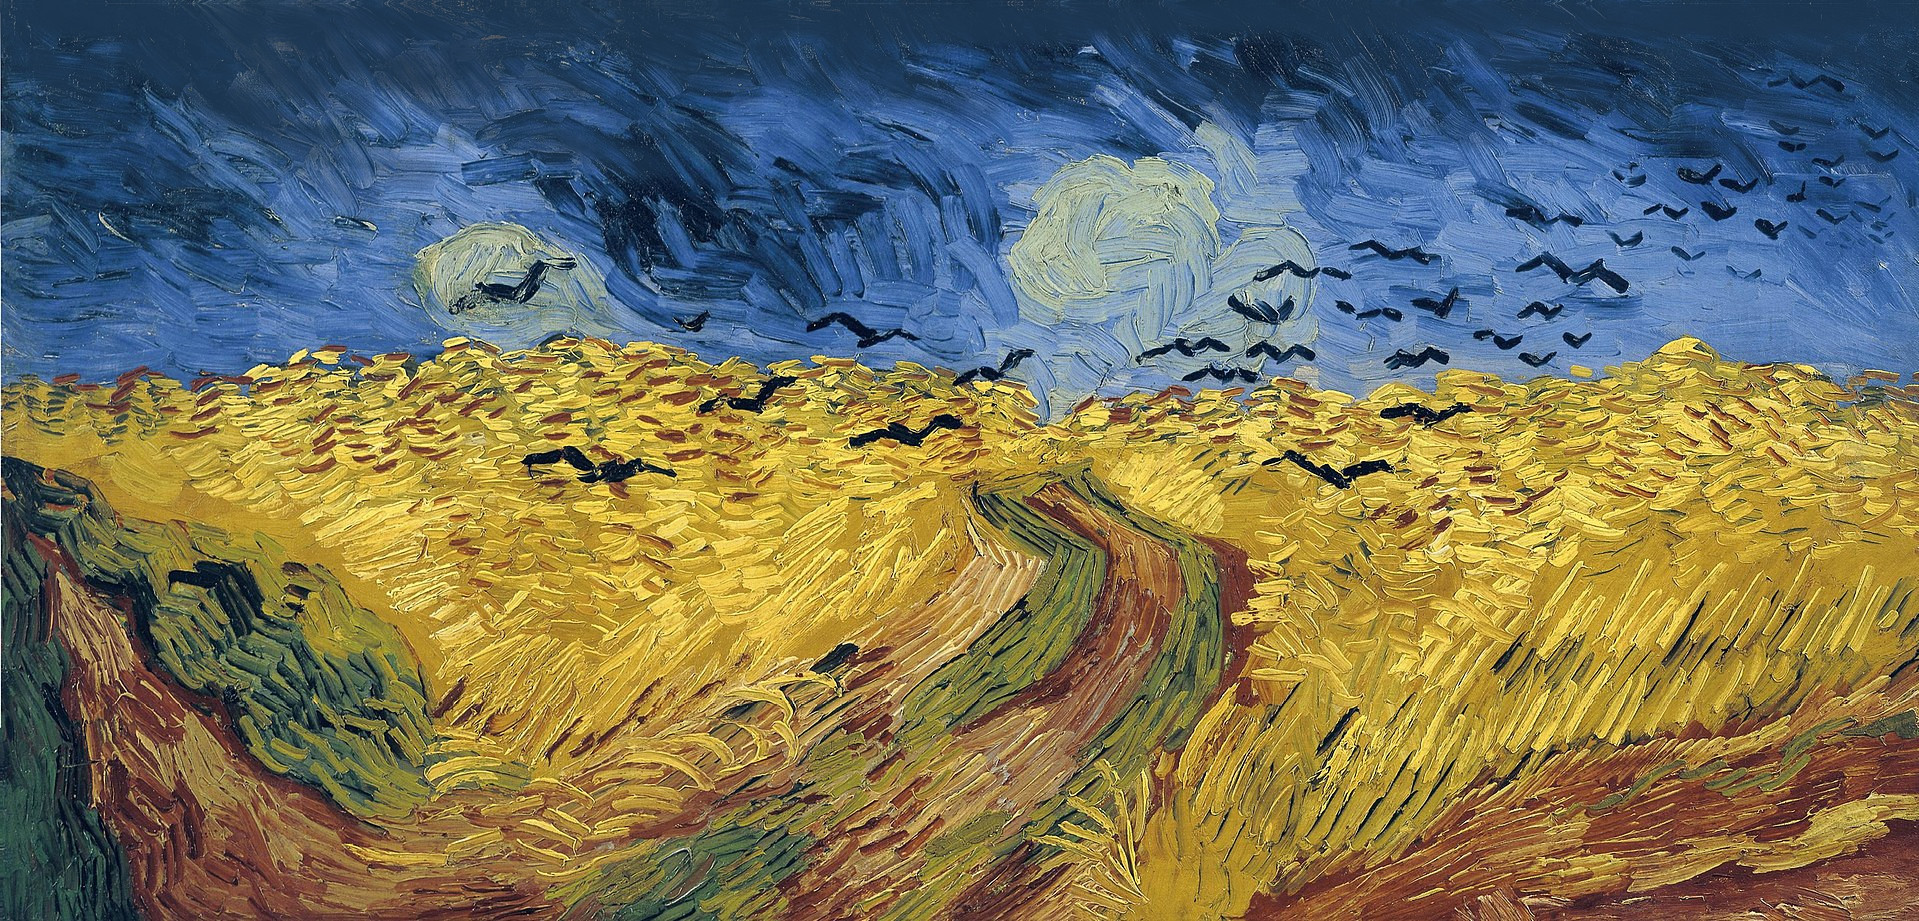
\includegraphics[width=\paperwidth]{ble2.jpg}}
};
\end{tikzpicture}
\end{center}

\clearpage
\newgeometry{left=2.5cm, right=2.5cm,top=3cm, bottom=3cm}
\pagenumbering{arabic}
\pagestyle{fancy}
\fancyhead{}\fancyfoot[C]{\thepage}
\section*{Résumé}
\setcounter{tocdepth}{6}
\renewcommand\contentsname{Sommaire}
\tableofcontents



\section*{Introduction}
\section{Analyse macroéconomique du blé et du nickel}
\subsection{Le blé}
\subsection{Le nickel}

\section{Analyse des séries chronologiques}
Les méthodes traditionnelles de prévision, reposent sur la décomposition des différentes composantes d'une série temporelle. Ici il s'agira donc
ici d'analyser ces différentes composantes (c'est à dire la tendance et la saisonnalité).
\subsection{Stabilité de la variance}
Afin de pouvoir travailler sur la série, il est nécessaire de réduire les 
fluctuations importantes de la série. Pour cela des test ARCH sont fait sur les 
séries initiales afin de déterminer si il y a homoscédasticité dans la distribution. L'hypothèse nulle et alternative sont :
\archtest{41}{27,31}{14,07}
\begin{table}[H]
    \centering
    {\sffamily
    \begin{tabular}{lcc}
        \toprule
        Série           &  $LM$ & $\rchi^{2}_{0,95} (7)$\\
        \midrule
        Blé (16-19)     & 27,30     & 14,07 \\ 
        Blé (16-21)     & 54,10     & 14,07\\
        \bottomrule
    \end{tabular}
    \begin{tabular}{lcc}
        \toprule
        Série           &  $LM$ & $\rchi^{2}_{0,95} (7)$\\
        \midrule
        Nickel (16-19)  & 21,40     & 14,07\\
        Nickel (16-21)  & 49,96     & 14,07\\
        \bottomrule
    \end{tabular}}
    \caption{Résultats du test ARCH}
\end{table}
Ici, pour toutes les séries, la statistique $LM$ est supérieur au seuil, l'hypothèse $H_{0}$ est 
rejetée au risque de $5\%$. Les cours du blé et du nickel sont donc présente de l'hétéroscédasticité. Afin d'amoindrir ces fluctuations importantes, une transformation 
logarithmique est faite sur chacune des séries. Les séries transformées serviront donc
pour le reste du travail.

\subsection{Analyse graphique et tableau de Buys-Ballot}\label{graph}
Dans un premier temps, une étude intuitive peut être faite. Il s'agira donc ici d'analyser graphiquement chacune des chroniques afin 
de déterminer de façon préliminaire, si les cours du blé et du nickel sont sujet à de la saisonnalité, et/ou de la tendance.

Pour le cours du blé, il est possible de déceler légère une tendance a la hausse de 2016 à 2019. Cette tendance s'accentue si 2020 et 2021 
sont inclus. Pour ce qui est de la saisonnalité, il semble impossible de déterminer que la série possède une quelconque saisonnalité
\textit{(figure~\ref{fig:ble_log} p.~\pageref{fig:ble_log})}.

Dans le cas du nickel, une tendance haussière se démarque (tout échantillon confondu). Quant à la saisonnalité, sur l'échantillon 2016-2019, 
la série ne semble pas saisonnière. Cependant sur l'échantillon 2016-2021, la série peut sembler saisonnière par périodes de un an.
\textit{(figure~\ref{fig:nickel_log} p.~\pageref{fig:nickel_log})}.

Les deux séries semblent donc se comporter de manière similaire : faible tendance haussière, ainsi que non saisonnières. 

\subsection{Analyse de la variance}
Afin de confirmer les intuitons développées en ~\ref{graph} une analyse de la variance et le test de Fisher sur la tendance et de 
saisonnalité doivent être menés. La détection de la saisonnalité est essentielle, car les méthodes de prévision traditionnelles
ne peuvent être que menées sur des séries non saisonnières ou bien désaisonnalisées.

L'analyse de la variance est basée sur les moyennes calculées dans le tableau de Buys Ballot. En effet afin d'analyser la saisonnalité, 
il reviendra a étudier l'influence du facteur colonne (variance des mois) et pour la tendance, l'influence du facteur ligne (variance des années).
Après calculs \textit{(Cf-\ref{appendix:anova} p.\pageref{appendix:anova})}, les différentes variances sont affichées dans le tableau ci-dessous.

\begin{table}[H]
    \centering
    \caption{Analyse de la variance}
    \sffamily
    \begin{tabular}{lcccc}
\toprule
\multirow{2}*{Échantillon}& \multicolumn{2}{c}{2016-2019}   & \multicolumn{2}{c}{2016-2021} \\
      &  Blé &  Nickel& Blé &  Nickel \\ 
\cmidrule(r){1-1}\cmidrule(lr){2-3}\cmidrule(l){4-5}
    Variance période                         & 0,0086      &   0,0129    & 0,0023       & 0,0243      \\
    Variance année                           & 0,2746      &   0,3723    & 0,0661       & 0,6502      \\
    Variance résidus                         & 0,0048      &   0,0286    & 0,0033       & 0,0098      \\ 
\bottomrule
\end{tabular}
\end{table}

Enfin grace aux variances, le test de fisher peut être effectué.

\subsubsection{Test de Fisher de détection de saisonnalité}
Il s'agira ici de tester l'influence du facteur colonne en comparant la variance période à la variance résiduelle
,afin de déterminer si les séries sont saisonnières.
\test{Pas d'influence du facteur colonne (pas de saisonnalité)}
    {Influence du facteur colonne (saisonnalité)}
    {F_{c} = \frac{V_{P}}{V_{R}} \sim F_{0,95}((n-1), (n-1)(p-1))}
La statistique calculée ($F_{c}$) est ensuite comparée au quantile à $95\%$ de la distribution $F$ de
Fisher avec comme degrés de liberté $(p-1)$ et $(n-1)(p-1)$, où $n$ représente le nombre d'année
et $p$ le nombre de périodes. Si la statistique empirique est supérieure au quantile,
alors $ H_{0} $ est rejetée, la série est saisonnière. Après calculs :
\begin{table}[H]
    \centering
    \caption{Test de Fisher (saisonnalité)}
    \sffamily
    \begin{tabular}{lcccc}
\toprule
    & \multicolumn{2}{c}{2016 -2019}   & \multicolumn{2}{c}{2016 -2021} \\
    & Blé  & Nickel & Blé  & Nickel \\
  \cmidrule(r){1-1}\cmidrule(lr){2-3}\cmidrule(l){4-5}
  $F_{c}$ & 0,6986  & 0,4505  &  1,7906 & 2,4772                     \\ 
  $F_{0,95}$ & 2,0933 & 2,0933	& 1,9675 & 1,9675\\
  \textit{ddl} &  (11;33)& (11;33) & (11;55) & (11;55)\\
  \bottomrule             
\end{tabular}
\end{table}
Ici, les statistique calculée sont toutes inférieures au seuil, sauf pour l'échantillon (2016-2021)
du nickel.  Ainsi, l'hypothèse $H_{0}$ est acceptée au risque de $5\%$ pour les deux échantillons du blé
et pour l'échantillon (2016-2019) du nickel. En revanche elle est rejetée pour l'échantillon (2016-2021) du nickel.\\[11pt]
Pour ses deux échantillons, la série du blé n'est donc pas saisonnière, il en est de même pour le premier échantillon de la série du nickel. 
Par contre, l'échantillon (2016-2021) du nickel est lui saisonnier, il faudra donc à la suite 
déterminer son type de saisonnalité (déterministe ou aléatoire), puis son type de schéma de décomposition
(additif ou multiplicatif) et finalement désaisonnaliser la série afin de pouvoir utiliser les méthodes de prévision.
\subsubsection{Test de Fisher de détection de tendance}
De manière analogue, il revient à comparer la variance année à la variance résiduelle afin de déterminer si les séries possèdent une tendance.
\test{Pas d'influence du facteur ligne (pas de tendance)}
    {Influence du facteur ligne (tendance)}
    {F_{c} = \frac{V_{A}}{V_{R}} \sim F_{0,95}((p-1), (n-1)(p-1))}
Comme pour le test précédent, si la statistique calculée est supérieure au quantile à $ 95\% $ 
de la distribution de Fisher ayant pour \textit{dll} : $(n-1)$ et $(n-1)(p-1)$ , alors $ H_{0} $ est rejetée, la série possède une tendance.
\begin{table}[H]
    \centering
    \caption{Test de Fisher (tendance)}
    \sffamily
    \begin{tabular}{lcccc}
    \toprule
         & \multicolumn{2}{c}{2016 -2019} & \multicolumn{2}{c}{2016 -2021}  \\
         & Blé      & Nickel    & Blé       & Nickel                        \\
    \cmidrule(r){1-1}\cmidrule(lr){2-3}\cmidrule(l){4-5}
        $F_{c}$     & 20,1576   & 12,9965   & 56,8388   & 66,2263           \\
        $F_{0,95}$  & 2,8916    & 2,8916    & 2,3828    & 2,3828            \\*
        \textit{ddl}& (3;33)    & (3;33)    & (5;55)    & (3;55)            \\
    \bottomrule
\end{tabular}

\end{table}
Ici dans tous les cas, le Fisher empirique est supérieur au Fisher théorique, $H_{0}$ est rejetée
au risque de $ 5\% $ pour toutes les séries. \\[11pt]
Les deux séries et leurs échantillons possèdent donc une tendance. Il à remarquer que la probabilité de rejeter 
$H_{0}$ est bien plus supérieure sur les échantillons (2016-2021) que sur les échantillons (2016-2019),
cela confirme l'intuition dégagée de l'analyse graphique.

\subsection{Analyse de la saisonnalité de l'échantillon (2016-2021) du nickel}
Comme vu précédemment l'échantillon (2016-2021) du Nickel possède de la saisonnalité, il est donc indispensable d'étudier, puis de corriger la saisonnalité. 
\subsubsection{Type de saisonnalité et schéma de décomposition}
Dans un premier temps le type de saisonnalité doit être défini, en effet la saisonnalité peut être déterministe ou bien aléatoire. Pour cela chaque ligne du tableau de 
Buys-Ballot de l'échantillon concerné est classée par ordre croissant. De plus pour faciliter la lecture, chaque mois s'est vu attribué une couleur appartenant à
un gradient rouge (\textit{tableau~\ref{tab:bbc} p.\pageref{tab:bbc} }). Il est donc rapidement possible de remarquer que la saisonnalité n'est pas répétitive,
elle est donc aléatoire. Il faudra donc désaisonnaliser la série par méthode CENSUS.\\[11pt] 



\section{Prévision par le méthodes traditionnelles}
\subsection{Prévision pour 2020}
\subsubsection{Lissage exponentiel double (LED)}
\subsubsection{Lissage exponentiel triple (Holt Winter)}
\subsubsection{Extrapolation d'une droite de tendance}
\subsection{Prévision pour 2022}
\subsubsection{Lissage exponentiel double (LED)}
\subsubsection{Lissage exponentiel triple (Holt Winter)}
\subsubsection{Extrapolation d'une droite de tendance}
\subsection{Classification des méthodes}
\subsubsection{Blé}
\subsubsection{Nickel}
\subsection{Prévision pour 2023}
\subsubsection{Blé}
\subsubsection{Nickel}
\section{Prévision selon la méthodologie de Box \& Jenkins}
\subsection{Présentation de la méthode}
\subsection{Test de racine unitaire}
\subsection{Identification des processus}
\subsection{Tests de validité}
\subsubsection{Significativité des paramètres}
\subsubsection{Tests sur les résidus}
\subsection{Prévision pour 2023}
\section*{Conclusion}


faire par sous périodes


\appendix
\renewcommand\thefigure{\thesubsubsection.\arabic{table}}
\renewcommand\thetable{\thesubsubsection.\arabic{figure}}    
\section{Analyse des séries chronologiques}
\subsection{Stabilité de la variance}\label{appendix:hetero}
\begin{table}[H]
    \sffamily
    \centering
    \label{tab:hetero_ble}
    \begin{tabular}{lrrrr}
\toprule
\multicolumn{2}{l}{Heteroskedasticity Test: ARCH}&\multicolumn{1}{c}{Echantillon}&\multicolumn{1}{c}{2016-2019}&\multicolumn{1}{c}{}\\
 \midrule 
\multicolumn{1}{l}{F-statistic}&\multicolumn{1}{r}{9.401617}&\multicolumn{2}{l}{Prob. F(7,33)}&\multicolumn{1}{r}{0.0000}\\
\multicolumn{1}{l}{Obs*R-squared}&\multicolumn{1}{r}{27.30724}&\multicolumn{2}{l}{Prob. Chi-Square(7)}&\multicolumn{1}{r}{0.0003}\\
 \toprule
\multicolumn{1}{c}{Heteroskedasticity Test: ARCH}&\multicolumn{1}{c}{}&\multicolumn{1}{c}{Echantillon}&\multicolumn{1}{c}{2016-2021}&\multicolumn{1}{c}{}\\
 \midrule
\multicolumn{1}{l}{F-statistic}&\multicolumn{1}{c}{40.42172}&\multicolumn{1}{l}{Prob. F(7,57)}&\multicolumn{1}{c}{}&\multicolumn{1}{c}{0.0000}\\
\multicolumn{1}{l}{Obs*R-squared}&\multicolumn{1}{c}{54.10140}&\multicolumn{1}{l}{Prob. Chi-Square(7)}&\multicolumn{1}{c}{}&\multicolumn{1}{c}{0.0000}\\
 \bottomrule
\end{tabular}
    \caption{Test ARCH pour la série Blé}
\end{table}
\begin{table}[H]
    \sffamily
    \centering
    \label{tab:hetero_nickel}
    \begin{tabular}{lrrrr}
\toprule
\multicolumn{2}{l}{Heteroskedasticity Test: ARCH}&\multicolumn{1}{c}{Echantillon}&\multicolumn{1}{c}{2016-2019}&\multicolumn{1}{c}{}\\
 \midrule
\multicolumn{1}{l}{F-statistic}&\multicolumn{1}{r}{5.151741}&\multicolumn{2}{l}{Prob. F(7,33)}&\multicolumn{1}{r}{0.0005}\\
\multicolumn{1}{l}{Obs*R-squared}&\multicolumn{1}{r}{21.40896}&\multicolumn{2}{l}{Prob. Chi-Square(7)}&\multicolumn{1}{r}{0.0032}\\
\toprule
\multicolumn{1}{l}{Heteroskedasticity Test: ARCH}&\multicolumn{1}{c}{}&\multicolumn{1}{c}{Echantillon}&\multicolumn{1}{c}{2016-2021}&\multicolumn{1}{c}{}\\
 \midrule
\multicolumn{1}{l}{F-statistic}&\multicolumn{1}{r}{27.04986}&\multicolumn{1}{l}{Prob. F(7,57)}&\multicolumn{1}{l}{}&\multicolumn{1}{c}{0.0000}\\
\multicolumn{1}{l}{Obs*R-squared}&\multicolumn{1}{r}{49.96036}&\multicolumn{1}{l}{Prob. Chi-Square(7)}&\multicolumn{1}{l}{}&\multicolumn{1}{c}{0.0000}\\
 \bottomrule
\end{tabular}

    \caption{Test ARCH pour la série Nickel}
\end{table}
\subsection{Analyse graphique}\label{appendix:loggraph}
\begin{figure}[H]
    \centering
    \label{fig:ble_log}
    \resizebox{0.6\textwidth}{!}{%% Creator: Matplotlib, PGF backend
%%
%% To include the figure in your LaTeX document, write
%%   \input{<filename>.pgf}
%%
%% Make sure the required packages are loaded in your preamble
%%   \usepackage{pgf}
%%
%% Also ensure that all the required font packages are loaded; for instance,
%% the lmodern package is sometimes necessary when using math font.
%%   \usepackage{lmodern}
%%
%% Figures using additional raster images can only be included by \input if
%% they are in the same directory as the main LaTeX file. For loading figures
%% from other directories you can use the `import` package
%%   \usepackage{import}
%%
%% and then include the figures with
%%   \import{<path to file>}{<filename>.pgf}
%%
%% Matplotlib used the following preamble
%%   \usepackage{fontspec}
%%   \setmainfont{DejaVuSerif.ttf}[Path=\detokenize{C:/Users/Joseph/miniconda3/Lib/site-packages/matplotlib/mpl-data/fonts/ttf/}]
%%   \setsansfont{arial.ttf}[Path=\detokenize{C:/Windows/Fonts/}]
%%   \setmonofont{DejaVuSansMono.ttf}[Path=\detokenize{C:/Users/Joseph/miniconda3/Lib/site-packages/matplotlib/mpl-data/fonts/ttf/}]
%%
\begingroup%
\makeatletter%
\begin{pgfpicture}%
\pgfpathrectangle{\pgfpointorigin}{\pgfqpoint{6.400000in}{4.800000in}}%
\pgfusepath{use as bounding box, clip}%
\begin{pgfscope}%
\pgfsetbuttcap%
\pgfsetmiterjoin%
\definecolor{currentfill}{rgb}{1.000000,1.000000,1.000000}%
\pgfsetfillcolor{currentfill}%
\pgfsetlinewidth{0.000000pt}%
\definecolor{currentstroke}{rgb}{1.000000,1.000000,1.000000}%
\pgfsetstrokecolor{currentstroke}%
\pgfsetdash{}{0pt}%
\pgfpathmoveto{\pgfqpoint{0.000000in}{0.000000in}}%
\pgfpathlineto{\pgfqpoint{6.400000in}{0.000000in}}%
\pgfpathlineto{\pgfqpoint{6.400000in}{4.800000in}}%
\pgfpathlineto{\pgfqpoint{0.000000in}{4.800000in}}%
\pgfpathlineto{\pgfqpoint{0.000000in}{0.000000in}}%
\pgfpathclose%
\pgfusepath{fill}%
\end{pgfscope}%
\begin{pgfscope}%
\pgfsetbuttcap%
\pgfsetmiterjoin%
\definecolor{currentfill}{rgb}{1.000000,1.000000,1.000000}%
\pgfsetfillcolor{currentfill}%
\pgfsetlinewidth{0.000000pt}%
\definecolor{currentstroke}{rgb}{0.000000,0.000000,0.000000}%
\pgfsetstrokecolor{currentstroke}%
\pgfsetstrokeopacity{0.000000}%
\pgfsetdash{}{0pt}%
\pgfpathmoveto{\pgfqpoint{0.800000in}{0.528000in}}%
\pgfpathlineto{\pgfqpoint{5.760000in}{0.528000in}}%
\pgfpathlineto{\pgfqpoint{5.760000in}{4.224000in}}%
\pgfpathlineto{\pgfqpoint{0.800000in}{4.224000in}}%
\pgfpathlineto{\pgfqpoint{0.800000in}{0.528000in}}%
\pgfpathclose%
\pgfusepath{fill}%
\end{pgfscope}%
\begin{pgfscope}%
\pgfsetbuttcap%
\pgfsetroundjoin%
\definecolor{currentfill}{rgb}{0.150000,0.150000,0.150000}%
\pgfsetfillcolor{currentfill}%
\pgfsetlinewidth{1.003750pt}%
\definecolor{currentstroke}{rgb}{0.150000,0.150000,0.150000}%
\pgfsetstrokecolor{currentstroke}%
\pgfsetdash{}{0pt}%
\pgfsys@defobject{currentmarker}{\pgfqpoint{0.000000in}{-0.066667in}}{\pgfqpoint{0.000000in}{0.000000in}}{%
\pgfpathmoveto{\pgfqpoint{0.000000in}{0.000000in}}%
\pgfpathlineto{\pgfqpoint{0.000000in}{-0.066667in}}%
\pgfusepath{stroke,fill}%
}%
\begin{pgfscope}%
\pgfsys@transformshift{1.580094in}{0.528000in}%
\pgfsys@useobject{currentmarker}{}%
\end{pgfscope}%
\end{pgfscope}%
\begin{pgfscope}%
\definecolor{textcolor}{rgb}{0.150000,0.150000,0.150000}%
\pgfsetstrokecolor{textcolor}%
\pgfsetfillcolor{textcolor}%
\pgftext[x=1.580094in,y=0.412722in,,top]{\color{textcolor}\sffamily\fontsize{8.800000}{10.560000}\selectfont 2017}%
\end{pgfscope}%
\begin{pgfscope}%
\pgfsetbuttcap%
\pgfsetroundjoin%
\definecolor{currentfill}{rgb}{0.150000,0.150000,0.150000}%
\pgfsetfillcolor{currentfill}%
\pgfsetlinewidth{1.003750pt}%
\definecolor{currentstroke}{rgb}{0.150000,0.150000,0.150000}%
\pgfsetstrokecolor{currentstroke}%
\pgfsetdash{}{0pt}%
\pgfsys@defobject{currentmarker}{\pgfqpoint{0.000000in}{-0.066667in}}{\pgfqpoint{0.000000in}{0.000000in}}{%
\pgfpathmoveto{\pgfqpoint{0.000000in}{0.000000in}}%
\pgfpathlineto{\pgfqpoint{0.000000in}{-0.066667in}}%
\pgfusepath{stroke,fill}%
}%
\begin{pgfscope}%
\pgfsys@transformshift{2.430047in}{0.528000in}%
\pgfsys@useobject{currentmarker}{}%
\end{pgfscope}%
\end{pgfscope}%
\begin{pgfscope}%
\definecolor{textcolor}{rgb}{0.150000,0.150000,0.150000}%
\pgfsetstrokecolor{textcolor}%
\pgfsetfillcolor{textcolor}%
\pgftext[x=2.430047in,y=0.412722in,,top]{\color{textcolor}\sffamily\fontsize{8.800000}{10.560000}\selectfont 2018}%
\end{pgfscope}%
\begin{pgfscope}%
\pgfsetbuttcap%
\pgfsetroundjoin%
\definecolor{currentfill}{rgb}{0.150000,0.150000,0.150000}%
\pgfsetfillcolor{currentfill}%
\pgfsetlinewidth{1.003750pt}%
\definecolor{currentstroke}{rgb}{0.150000,0.150000,0.150000}%
\pgfsetstrokecolor{currentstroke}%
\pgfsetdash{}{0pt}%
\pgfsys@defobject{currentmarker}{\pgfqpoint{0.000000in}{-0.066667in}}{\pgfqpoint{0.000000in}{0.000000in}}{%
\pgfpathmoveto{\pgfqpoint{0.000000in}{0.000000in}}%
\pgfpathlineto{\pgfqpoint{0.000000in}{-0.066667in}}%
\pgfusepath{stroke,fill}%
}%
\begin{pgfscope}%
\pgfsys@transformshift{3.280000in}{0.528000in}%
\pgfsys@useobject{currentmarker}{}%
\end{pgfscope}%
\end{pgfscope}%
\begin{pgfscope}%
\definecolor{textcolor}{rgb}{0.150000,0.150000,0.150000}%
\pgfsetstrokecolor{textcolor}%
\pgfsetfillcolor{textcolor}%
\pgftext[x=3.280000in,y=0.412722in,,top]{\color{textcolor}\sffamily\fontsize{8.800000}{10.560000}\selectfont 2019}%
\end{pgfscope}%
\begin{pgfscope}%
\pgfsetbuttcap%
\pgfsetroundjoin%
\definecolor{currentfill}{rgb}{0.150000,0.150000,0.150000}%
\pgfsetfillcolor{currentfill}%
\pgfsetlinewidth{1.003750pt}%
\definecolor{currentstroke}{rgb}{0.150000,0.150000,0.150000}%
\pgfsetstrokecolor{currentstroke}%
\pgfsetdash{}{0pt}%
\pgfsys@defobject{currentmarker}{\pgfqpoint{0.000000in}{-0.066667in}}{\pgfqpoint{0.000000in}{0.000000in}}{%
\pgfpathmoveto{\pgfqpoint{0.000000in}{0.000000in}}%
\pgfpathlineto{\pgfqpoint{0.000000in}{-0.066667in}}%
\pgfusepath{stroke,fill}%
}%
\begin{pgfscope}%
\pgfsys@transformshift{4.129953in}{0.528000in}%
\pgfsys@useobject{currentmarker}{}%
\end{pgfscope}%
\end{pgfscope}%
\begin{pgfscope}%
\definecolor{textcolor}{rgb}{0.150000,0.150000,0.150000}%
\pgfsetstrokecolor{textcolor}%
\pgfsetfillcolor{textcolor}%
\pgftext[x=4.129953in,y=0.412722in,,top]{\color{textcolor}\sffamily\fontsize{8.800000}{10.560000}\selectfont 2020}%
\end{pgfscope}%
\begin{pgfscope}%
\pgfsetbuttcap%
\pgfsetroundjoin%
\definecolor{currentfill}{rgb}{0.150000,0.150000,0.150000}%
\pgfsetfillcolor{currentfill}%
\pgfsetlinewidth{1.003750pt}%
\definecolor{currentstroke}{rgb}{0.150000,0.150000,0.150000}%
\pgfsetstrokecolor{currentstroke}%
\pgfsetdash{}{0pt}%
\pgfsys@defobject{currentmarker}{\pgfqpoint{0.000000in}{-0.066667in}}{\pgfqpoint{0.000000in}{0.000000in}}{%
\pgfpathmoveto{\pgfqpoint{0.000000in}{0.000000in}}%
\pgfpathlineto{\pgfqpoint{0.000000in}{-0.066667in}}%
\pgfusepath{stroke,fill}%
}%
\begin{pgfscope}%
\pgfsys@transformshift{4.982235in}{0.528000in}%
\pgfsys@useobject{currentmarker}{}%
\end{pgfscope}%
\end{pgfscope}%
\begin{pgfscope}%
\definecolor{textcolor}{rgb}{0.150000,0.150000,0.150000}%
\pgfsetstrokecolor{textcolor}%
\pgfsetfillcolor{textcolor}%
\pgftext[x=4.982235in,y=0.412722in,,top]{\color{textcolor}\sffamily\fontsize{8.800000}{10.560000}\selectfont 2021}%
\end{pgfscope}%
\begin{pgfscope}%
\definecolor{textcolor}{rgb}{0.150000,0.150000,0.150000}%
\pgfsetstrokecolor{textcolor}%
\pgfsetfillcolor{textcolor}%
\pgftext[x=3.280000in,y=0.245388in,,top]{\color{textcolor}\sffamily\fontsize{9.600000}{11.520000}\selectfont Date}%
\end{pgfscope}%
\begin{pgfscope}%
\pgfsetbuttcap%
\pgfsetroundjoin%
\definecolor{currentfill}{rgb}{0.150000,0.150000,0.150000}%
\pgfsetfillcolor{currentfill}%
\pgfsetlinewidth{1.003750pt}%
\definecolor{currentstroke}{rgb}{0.150000,0.150000,0.150000}%
\pgfsetstrokecolor{currentstroke}%
\pgfsetdash{}{0pt}%
\pgfsys@defobject{currentmarker}{\pgfqpoint{-0.066667in}{0.000000in}}{\pgfqpoint{-0.000000in}{0.000000in}}{%
\pgfpathmoveto{\pgfqpoint{-0.000000in}{0.000000in}}%
\pgfpathlineto{\pgfqpoint{-0.066667in}{0.000000in}}%
\pgfusepath{stroke,fill}%
}%
\begin{pgfscope}%
\pgfsys@transformshift{0.800000in}{0.528000in}%
\pgfsys@useobject{currentmarker}{}%
\end{pgfscope}%
\end{pgfscope}%
\begin{pgfscope}%
\definecolor{textcolor}{rgb}{0.150000,0.150000,0.150000}%
\pgfsetstrokecolor{textcolor}%
\pgfsetfillcolor{textcolor}%
\pgftext[x=0.514816in, y=0.484255in, left, base]{\color{textcolor}\sffamily\fontsize{8.800000}{10.560000}\selectfont 4.9}%
\end{pgfscope}%
\begin{pgfscope}%
\pgfsetbuttcap%
\pgfsetroundjoin%
\definecolor{currentfill}{rgb}{0.150000,0.150000,0.150000}%
\pgfsetfillcolor{currentfill}%
\pgfsetlinewidth{1.003750pt}%
\definecolor{currentstroke}{rgb}{0.150000,0.150000,0.150000}%
\pgfsetstrokecolor{currentstroke}%
\pgfsetdash{}{0pt}%
\pgfsys@defobject{currentmarker}{\pgfqpoint{-0.066667in}{0.000000in}}{\pgfqpoint{-0.000000in}{0.000000in}}{%
\pgfpathmoveto{\pgfqpoint{-0.000000in}{0.000000in}}%
\pgfpathlineto{\pgfqpoint{-0.066667in}{0.000000in}}%
\pgfusepath{stroke,fill}%
}%
\begin{pgfscope}%
\pgfsys@transformshift{0.800000in}{0.990000in}%
\pgfsys@useobject{currentmarker}{}%
\end{pgfscope}%
\end{pgfscope}%
\begin{pgfscope}%
\definecolor{textcolor}{rgb}{0.150000,0.150000,0.150000}%
\pgfsetstrokecolor{textcolor}%
\pgfsetfillcolor{textcolor}%
\pgftext[x=0.514816in, y=0.946255in, left, base]{\color{textcolor}\sffamily\fontsize{8.800000}{10.560000}\selectfont 5.0}%
\end{pgfscope}%
\begin{pgfscope}%
\pgfsetbuttcap%
\pgfsetroundjoin%
\definecolor{currentfill}{rgb}{0.150000,0.150000,0.150000}%
\pgfsetfillcolor{currentfill}%
\pgfsetlinewidth{1.003750pt}%
\definecolor{currentstroke}{rgb}{0.150000,0.150000,0.150000}%
\pgfsetstrokecolor{currentstroke}%
\pgfsetdash{}{0pt}%
\pgfsys@defobject{currentmarker}{\pgfqpoint{-0.066667in}{0.000000in}}{\pgfqpoint{-0.000000in}{0.000000in}}{%
\pgfpathmoveto{\pgfqpoint{-0.000000in}{0.000000in}}%
\pgfpathlineto{\pgfqpoint{-0.066667in}{0.000000in}}%
\pgfusepath{stroke,fill}%
}%
\begin{pgfscope}%
\pgfsys@transformshift{0.800000in}{1.452000in}%
\pgfsys@useobject{currentmarker}{}%
\end{pgfscope}%
\end{pgfscope}%
\begin{pgfscope}%
\definecolor{textcolor}{rgb}{0.150000,0.150000,0.150000}%
\pgfsetstrokecolor{textcolor}%
\pgfsetfillcolor{textcolor}%
\pgftext[x=0.514816in, y=1.408255in, left, base]{\color{textcolor}\sffamily\fontsize{8.800000}{10.560000}\selectfont 5.1}%
\end{pgfscope}%
\begin{pgfscope}%
\pgfsetbuttcap%
\pgfsetroundjoin%
\definecolor{currentfill}{rgb}{0.150000,0.150000,0.150000}%
\pgfsetfillcolor{currentfill}%
\pgfsetlinewidth{1.003750pt}%
\definecolor{currentstroke}{rgb}{0.150000,0.150000,0.150000}%
\pgfsetstrokecolor{currentstroke}%
\pgfsetdash{}{0pt}%
\pgfsys@defobject{currentmarker}{\pgfqpoint{-0.066667in}{0.000000in}}{\pgfqpoint{-0.000000in}{0.000000in}}{%
\pgfpathmoveto{\pgfqpoint{-0.000000in}{0.000000in}}%
\pgfpathlineto{\pgfqpoint{-0.066667in}{0.000000in}}%
\pgfusepath{stroke,fill}%
}%
\begin{pgfscope}%
\pgfsys@transformshift{0.800000in}{1.914000in}%
\pgfsys@useobject{currentmarker}{}%
\end{pgfscope}%
\end{pgfscope}%
\begin{pgfscope}%
\definecolor{textcolor}{rgb}{0.150000,0.150000,0.150000}%
\pgfsetstrokecolor{textcolor}%
\pgfsetfillcolor{textcolor}%
\pgftext[x=0.514816in, y=1.870255in, left, base]{\color{textcolor}\sffamily\fontsize{8.800000}{10.560000}\selectfont 5.2}%
\end{pgfscope}%
\begin{pgfscope}%
\pgfsetbuttcap%
\pgfsetroundjoin%
\definecolor{currentfill}{rgb}{0.150000,0.150000,0.150000}%
\pgfsetfillcolor{currentfill}%
\pgfsetlinewidth{1.003750pt}%
\definecolor{currentstroke}{rgb}{0.150000,0.150000,0.150000}%
\pgfsetstrokecolor{currentstroke}%
\pgfsetdash{}{0pt}%
\pgfsys@defobject{currentmarker}{\pgfqpoint{-0.066667in}{0.000000in}}{\pgfqpoint{-0.000000in}{0.000000in}}{%
\pgfpathmoveto{\pgfqpoint{-0.000000in}{0.000000in}}%
\pgfpathlineto{\pgfqpoint{-0.066667in}{0.000000in}}%
\pgfusepath{stroke,fill}%
}%
\begin{pgfscope}%
\pgfsys@transformshift{0.800000in}{2.376000in}%
\pgfsys@useobject{currentmarker}{}%
\end{pgfscope}%
\end{pgfscope}%
\begin{pgfscope}%
\definecolor{textcolor}{rgb}{0.150000,0.150000,0.150000}%
\pgfsetstrokecolor{textcolor}%
\pgfsetfillcolor{textcolor}%
\pgftext[x=0.514816in, y=2.332255in, left, base]{\color{textcolor}\sffamily\fontsize{8.800000}{10.560000}\selectfont 5.3}%
\end{pgfscope}%
\begin{pgfscope}%
\pgfsetbuttcap%
\pgfsetroundjoin%
\definecolor{currentfill}{rgb}{0.150000,0.150000,0.150000}%
\pgfsetfillcolor{currentfill}%
\pgfsetlinewidth{1.003750pt}%
\definecolor{currentstroke}{rgb}{0.150000,0.150000,0.150000}%
\pgfsetstrokecolor{currentstroke}%
\pgfsetdash{}{0pt}%
\pgfsys@defobject{currentmarker}{\pgfqpoint{-0.066667in}{0.000000in}}{\pgfqpoint{-0.000000in}{0.000000in}}{%
\pgfpathmoveto{\pgfqpoint{-0.000000in}{0.000000in}}%
\pgfpathlineto{\pgfqpoint{-0.066667in}{0.000000in}}%
\pgfusepath{stroke,fill}%
}%
\begin{pgfscope}%
\pgfsys@transformshift{0.800000in}{2.838000in}%
\pgfsys@useobject{currentmarker}{}%
\end{pgfscope}%
\end{pgfscope}%
\begin{pgfscope}%
\definecolor{textcolor}{rgb}{0.150000,0.150000,0.150000}%
\pgfsetstrokecolor{textcolor}%
\pgfsetfillcolor{textcolor}%
\pgftext[x=0.514816in, y=2.794255in, left, base]{\color{textcolor}\sffamily\fontsize{8.800000}{10.560000}\selectfont 5.4}%
\end{pgfscope}%
\begin{pgfscope}%
\pgfsetbuttcap%
\pgfsetroundjoin%
\definecolor{currentfill}{rgb}{0.150000,0.150000,0.150000}%
\pgfsetfillcolor{currentfill}%
\pgfsetlinewidth{1.003750pt}%
\definecolor{currentstroke}{rgb}{0.150000,0.150000,0.150000}%
\pgfsetstrokecolor{currentstroke}%
\pgfsetdash{}{0pt}%
\pgfsys@defobject{currentmarker}{\pgfqpoint{-0.066667in}{0.000000in}}{\pgfqpoint{-0.000000in}{0.000000in}}{%
\pgfpathmoveto{\pgfqpoint{-0.000000in}{0.000000in}}%
\pgfpathlineto{\pgfqpoint{-0.066667in}{0.000000in}}%
\pgfusepath{stroke,fill}%
}%
\begin{pgfscope}%
\pgfsys@transformshift{0.800000in}{3.300000in}%
\pgfsys@useobject{currentmarker}{}%
\end{pgfscope}%
\end{pgfscope}%
\begin{pgfscope}%
\definecolor{textcolor}{rgb}{0.150000,0.150000,0.150000}%
\pgfsetstrokecolor{textcolor}%
\pgfsetfillcolor{textcolor}%
\pgftext[x=0.514816in, y=3.256255in, left, base]{\color{textcolor}\sffamily\fontsize{8.800000}{10.560000}\selectfont 5.5}%
\end{pgfscope}%
\begin{pgfscope}%
\pgfsetbuttcap%
\pgfsetroundjoin%
\definecolor{currentfill}{rgb}{0.150000,0.150000,0.150000}%
\pgfsetfillcolor{currentfill}%
\pgfsetlinewidth{1.003750pt}%
\definecolor{currentstroke}{rgb}{0.150000,0.150000,0.150000}%
\pgfsetstrokecolor{currentstroke}%
\pgfsetdash{}{0pt}%
\pgfsys@defobject{currentmarker}{\pgfqpoint{-0.066667in}{0.000000in}}{\pgfqpoint{-0.000000in}{0.000000in}}{%
\pgfpathmoveto{\pgfqpoint{-0.000000in}{0.000000in}}%
\pgfpathlineto{\pgfqpoint{-0.066667in}{0.000000in}}%
\pgfusepath{stroke,fill}%
}%
\begin{pgfscope}%
\pgfsys@transformshift{0.800000in}{3.762000in}%
\pgfsys@useobject{currentmarker}{}%
\end{pgfscope}%
\end{pgfscope}%
\begin{pgfscope}%
\definecolor{textcolor}{rgb}{0.150000,0.150000,0.150000}%
\pgfsetstrokecolor{textcolor}%
\pgfsetfillcolor{textcolor}%
\pgftext[x=0.514816in, y=3.718255in, left, base]{\color{textcolor}\sffamily\fontsize{8.800000}{10.560000}\selectfont 5.6}%
\end{pgfscope}%
\begin{pgfscope}%
\pgfsetbuttcap%
\pgfsetroundjoin%
\definecolor{currentfill}{rgb}{0.150000,0.150000,0.150000}%
\pgfsetfillcolor{currentfill}%
\pgfsetlinewidth{1.003750pt}%
\definecolor{currentstroke}{rgb}{0.150000,0.150000,0.150000}%
\pgfsetstrokecolor{currentstroke}%
\pgfsetdash{}{0pt}%
\pgfsys@defobject{currentmarker}{\pgfqpoint{-0.066667in}{0.000000in}}{\pgfqpoint{-0.000000in}{0.000000in}}{%
\pgfpathmoveto{\pgfqpoint{-0.000000in}{0.000000in}}%
\pgfpathlineto{\pgfqpoint{-0.066667in}{0.000000in}}%
\pgfusepath{stroke,fill}%
}%
\begin{pgfscope}%
\pgfsys@transformshift{0.800000in}{4.224000in}%
\pgfsys@useobject{currentmarker}{}%
\end{pgfscope}%
\end{pgfscope}%
\begin{pgfscope}%
\definecolor{textcolor}{rgb}{0.150000,0.150000,0.150000}%
\pgfsetstrokecolor{textcolor}%
\pgfsetfillcolor{textcolor}%
\pgftext[x=0.514816in, y=4.180255in, left, base]{\color{textcolor}\sffamily\fontsize{8.800000}{10.560000}\selectfont 5.7}%
\end{pgfscope}%
\begin{pgfscope}%
\definecolor{textcolor}{rgb}{0.150000,0.150000,0.150000}%
\pgfsetstrokecolor{textcolor}%
\pgfsetfillcolor{textcolor}%
\pgftext[x=0.459261in,y=2.376000in,,bottom,rotate=90.000000]{\color{textcolor}\sffamily\fontsize{9.600000}{11.520000}\selectfont Cours (log)}%
\end{pgfscope}%
\begin{pgfscope}%
\pgfpathrectangle{\pgfqpoint{0.800000in}{0.528000in}}{\pgfqpoint{4.960000in}{3.696000in}}%
\pgfusepath{clip}%
\pgfsetroundcap%
\pgfsetroundjoin%
\pgfsetlinewidth{1.204500pt}%
\definecolor{currentstroke}{rgb}{0.860000,0.371200,0.340000}%
\pgfsetstrokecolor{currentstroke}%
\pgfsetdash{}{0pt}%
\pgfpathmoveto{\pgfqpoint{0.790000in}{1.021623in}}%
\pgfpathlineto{\pgfqpoint{0.800000in}{0.953649in}}%
\pgfpathlineto{\pgfqpoint{0.867531in}{1.123068in}}%
\pgfpathlineto{\pgfqpoint{0.939718in}{1.085106in}}%
\pgfpathlineto{\pgfqpoint{1.009577in}{1.472463in}}%
\pgfpathlineto{\pgfqpoint{1.081765in}{1.212925in}}%
\pgfpathlineto{\pgfqpoint{1.151624in}{1.507384in}}%
\pgfpathlineto{\pgfqpoint{1.223812in}{1.183166in}}%
\pgfpathlineto{\pgfqpoint{1.296000in}{1.351718in}}%
\pgfpathlineto{\pgfqpoint{1.365859in}{1.500421in}}%
\pgfpathlineto{\pgfqpoint{1.438047in}{1.394695in}}%
\pgfpathlineto{\pgfqpoint{1.507906in}{1.562714in}}%
\pgfpathlineto{\pgfqpoint{1.580094in}{1.493447in}}%
\pgfpathlineto{\pgfqpoint{1.652282in}{1.678135in}}%
\pgfpathlineto{\pgfqpoint{1.717484in}{1.465447in}}%
\pgfpathlineto{\pgfqpoint{1.789671in}{1.569583in}}%
\pgfpathlineto{\pgfqpoint{1.859531in}{1.528210in}}%
\pgfpathlineto{\pgfqpoint{1.931718in}{1.790742in}}%
\pgfpathlineto{\pgfqpoint{2.001577in}{1.569583in}}%
\pgfpathlineto{\pgfqpoint{2.073765in}{1.212925in}}%
\pgfpathlineto{\pgfqpoint{2.145953in}{1.507384in}}%
\pgfpathlineto{\pgfqpoint{2.215812in}{1.394695in}}%
\pgfpathlineto{\pgfqpoint{2.288000in}{1.322843in}}%
\pgfpathlineto{\pgfqpoint{2.357859in}{1.308337in}}%
\pgfpathlineto{\pgfqpoint{2.430047in}{1.286493in}}%
\pgfpathlineto{\pgfqpoint{2.502235in}{1.528210in}}%
\pgfpathlineto{\pgfqpoint{2.567437in}{1.444335in}}%
\pgfpathlineto{\pgfqpoint{2.639624in}{1.569583in}}%
\pgfpathlineto{\pgfqpoint{2.709484in}{1.951510in}}%
\pgfpathlineto{\pgfqpoint{2.781671in}{1.842799in}}%
\pgfpathlineto{\pgfqpoint{2.851531in}{2.419911in}}%
\pgfpathlineto{\pgfqpoint{2.923718in}{2.476669in}}%
\pgfpathlineto{\pgfqpoint{2.995906in}{2.402747in}}%
\pgfpathlineto{\pgfqpoint{3.065765in}{2.333446in}}%
\pgfpathlineto{\pgfqpoint{3.137953in}{2.397011in}}%
\pgfpathlineto{\pgfqpoint{3.207812in}{2.442698in}}%
\pgfpathlineto{\pgfqpoint{3.280000in}{2.465373in}}%
\pgfpathlineto{\pgfqpoint{3.352188in}{2.209609in}}%
\pgfpathlineto{\pgfqpoint{3.417390in}{2.026736in}}%
\pgfpathlineto{\pgfqpoint{3.489577in}{1.964133in}}%
\pgfpathlineto{\pgfqpoint{3.559437in}{2.014283in}}%
\pgfpathlineto{\pgfqpoint{3.631624in}{1.887873in}}%
\pgfpathlineto{\pgfqpoint{3.701484in}{1.744706in}}%
\pgfpathlineto{\pgfqpoint{3.773671in}{1.458420in}}%
\pgfpathlineto{\pgfqpoint{3.845859in}{1.744706in}}%
\pgfpathlineto{\pgfqpoint{3.915718in}{1.829840in}}%
\pgfpathlineto{\pgfqpoint{3.987906in}{2.020514in}}%
\pgfpathlineto{\pgfqpoint{4.057765in}{2.100756in}}%
\pgfpathlineto{\pgfqpoint{4.129953in}{2.155503in}}%
\pgfpathlineto{\pgfqpoint{4.202141in}{2.070058in}}%
\pgfpathlineto{\pgfqpoint{4.269671in}{2.280779in}}%
\pgfpathlineto{\pgfqpoint{4.341859in}{2.268993in}}%
\pgfpathlineto{\pgfqpoint{4.411718in}{2.088501in}}%
\pgfpathlineto{\pgfqpoint{4.483906in}{1.894276in}}%
\pgfpathlineto{\pgfqpoint{4.553765in}{1.951510in}}%
\pgfpathlineto{\pgfqpoint{4.625953in}{2.076214in}}%
\pgfpathlineto{\pgfqpoint{4.698141in}{2.315957in}}%
\pgfpathlineto{\pgfqpoint{4.768000in}{2.487937in}}%
\pgfpathlineto{\pgfqpoint{4.840188in}{2.599134in}}%
\pgfpathlineto{\pgfqpoint{4.910047in}{2.664589in}}%
\pgfpathlineto{\pgfqpoint{4.982235in}{2.953269in}}%
\pgfpathlineto{\pgfqpoint{5.054423in}{3.305813in}}%
\pgfpathlineto{\pgfqpoint{5.119624in}{2.713079in}}%
\pgfpathlineto{\pgfqpoint{5.191812in}{3.540194in}}%
\pgfpathlineto{\pgfqpoint{5.261671in}{2.675409in}}%
\pgfpathlineto{\pgfqpoint{5.333859in}{2.577107in}}%
\pgfpathlineto{\pgfqpoint{5.403718in}{2.876310in}}%
\pgfpathlineto{\pgfqpoint{5.475906in}{3.375991in}}%
\pgfpathlineto{\pgfqpoint{5.548094in}{3.544673in}}%
\pgfpathlineto{\pgfqpoint{5.617953in}{3.976044in}}%
\pgfpathlineto{\pgfqpoint{5.690141in}{3.914471in}}%
\pgfpathlineto{\pgfqpoint{5.760000in}{3.897911in}}%
\pgfusepath{stroke}%
\end{pgfscope}%
\begin{pgfscope}%
\pgfsetrectcap%
\pgfsetmiterjoin%
\pgfsetlinewidth{1.003750pt}%
\definecolor{currentstroke}{rgb}{0.150000,0.150000,0.150000}%
\pgfsetstrokecolor{currentstroke}%
\pgfsetdash{}{0pt}%
\pgfpathmoveto{\pgfqpoint{0.800000in}{0.528000in}}%
\pgfpathlineto{\pgfqpoint{0.800000in}{4.224000in}}%
\pgfusepath{stroke}%
\end{pgfscope}%
\begin{pgfscope}%
\pgfsetrectcap%
\pgfsetmiterjoin%
\pgfsetlinewidth{1.003750pt}%
\definecolor{currentstroke}{rgb}{0.150000,0.150000,0.150000}%
\pgfsetstrokecolor{currentstroke}%
\pgfsetdash{}{0pt}%
\pgfpathmoveto{\pgfqpoint{0.800000in}{0.528000in}}%
\pgfpathlineto{\pgfqpoint{5.760000in}{0.528000in}}%
\pgfusepath{stroke}%
\end{pgfscope}%
\end{pgfpicture}%
\makeatother%
\endgroup%
}
    \caption{Cours du blé (en logarithme)}
\end{figure}
\begin{figure}[H]
    \centering
    \label{fig:nickel_log}
    \resizebox{0.6\textwidth}{!}{%% Creator: Matplotlib, PGF backend
%%
%% To include the figure in your LaTeX document, write
%%   \input{<filename>.pgf}
%%
%% Make sure the required packages are loaded in your preamble
%%   \usepackage{pgf}
%%
%% Also ensure that all the required font packages are loaded; for instance,
%% the lmodern package is sometimes necessary when using math font.
%%   \usepackage{lmodern}
%%
%% Figures using additional raster images can only be included by \input if
%% they are in the same directory as the main LaTeX file. For loading figures
%% from other directories you can use the `import` package
%%   \usepackage{import}
%%
%% and then include the figures with
%%   \import{<path to file>}{<filename>.pgf}
%%
%% Matplotlib used the following preamble
%%   \usepackage{fontspec}
%%   \setmainfont{DejaVuSerif.ttf}[Path=\detokenize{C:/Users/Joseph/miniconda3/Lib/site-packages/matplotlib/mpl-data/fonts/ttf/}]
%%   \setsansfont{arial.ttf}[Path=\detokenize{C:/Windows/Fonts/}]
%%   \setmonofont{DejaVuSansMono.ttf}[Path=\detokenize{C:/Users/Joseph/miniconda3/Lib/site-packages/matplotlib/mpl-data/fonts/ttf/}]
%%
\begingroup%
\makeatletter%
\begin{pgfpicture}%
\pgfpathrectangle{\pgfpointorigin}{\pgfqpoint{6.400000in}{4.800000in}}%
\pgfusepath{use as bounding box, clip}%
\begin{pgfscope}%
\pgfsetbuttcap%
\pgfsetmiterjoin%
\definecolor{currentfill}{rgb}{1.000000,1.000000,1.000000}%
\pgfsetfillcolor{currentfill}%
\pgfsetlinewidth{0.000000pt}%
\definecolor{currentstroke}{rgb}{1.000000,1.000000,1.000000}%
\pgfsetstrokecolor{currentstroke}%
\pgfsetdash{}{0pt}%
\pgfpathmoveto{\pgfqpoint{0.000000in}{0.000000in}}%
\pgfpathlineto{\pgfqpoint{6.400000in}{0.000000in}}%
\pgfpathlineto{\pgfqpoint{6.400000in}{4.800000in}}%
\pgfpathlineto{\pgfqpoint{0.000000in}{4.800000in}}%
\pgfpathlineto{\pgfqpoint{0.000000in}{0.000000in}}%
\pgfpathclose%
\pgfusepath{fill}%
\end{pgfscope}%
\begin{pgfscope}%
\pgfsetbuttcap%
\pgfsetmiterjoin%
\definecolor{currentfill}{rgb}{1.000000,1.000000,1.000000}%
\pgfsetfillcolor{currentfill}%
\pgfsetlinewidth{0.000000pt}%
\definecolor{currentstroke}{rgb}{0.000000,0.000000,0.000000}%
\pgfsetstrokecolor{currentstroke}%
\pgfsetstrokeopacity{0.000000}%
\pgfsetdash{}{0pt}%
\pgfpathmoveto{\pgfqpoint{0.800000in}{0.528000in}}%
\pgfpathlineto{\pgfqpoint{5.760000in}{0.528000in}}%
\pgfpathlineto{\pgfqpoint{5.760000in}{4.224000in}}%
\pgfpathlineto{\pgfqpoint{0.800000in}{4.224000in}}%
\pgfpathlineto{\pgfqpoint{0.800000in}{0.528000in}}%
\pgfpathclose%
\pgfusepath{fill}%
\end{pgfscope}%
\begin{pgfscope}%
\pgfpathrectangle{\pgfqpoint{0.800000in}{0.528000in}}{\pgfqpoint{4.960000in}{3.696000in}}%
\pgfusepath{clip}%
\pgfsetroundcap%
\pgfsetroundjoin%
\pgfsetlinewidth{1.003750pt}%
\definecolor{currentstroke}{rgb}{0.800000,0.800000,0.800000}%
\pgfsetstrokecolor{currentstroke}%
\pgfsetstrokeopacity{0.000000}%
\pgfsetdash{}{0pt}%
\pgfpathmoveto{\pgfqpoint{1.580094in}{0.528000in}}%
\pgfpathlineto{\pgfqpoint{1.580094in}{4.224000in}}%
\pgfusepath{stroke}%
\end{pgfscope}%
\begin{pgfscope}%
\definecolor{textcolor}{rgb}{0.150000,0.150000,0.150000}%
\pgfsetstrokecolor{textcolor}%
\pgfsetfillcolor{textcolor}%
\pgftext[x=1.580094in,y=0.396056in,,top]{\color{textcolor}\sffamily\fontsize{11.000000}{13.200000}\selectfont 2017}%
\end{pgfscope}%
\begin{pgfscope}%
\pgfpathrectangle{\pgfqpoint{0.800000in}{0.528000in}}{\pgfqpoint{4.960000in}{3.696000in}}%
\pgfusepath{clip}%
\pgfsetroundcap%
\pgfsetroundjoin%
\pgfsetlinewidth{1.003750pt}%
\definecolor{currentstroke}{rgb}{0.800000,0.800000,0.800000}%
\pgfsetstrokecolor{currentstroke}%
\pgfsetstrokeopacity{0.000000}%
\pgfsetdash{}{0pt}%
\pgfpathmoveto{\pgfqpoint{2.430047in}{0.528000in}}%
\pgfpathlineto{\pgfqpoint{2.430047in}{4.224000in}}%
\pgfusepath{stroke}%
\end{pgfscope}%
\begin{pgfscope}%
\definecolor{textcolor}{rgb}{0.150000,0.150000,0.150000}%
\pgfsetstrokecolor{textcolor}%
\pgfsetfillcolor{textcolor}%
\pgftext[x=2.430047in,y=0.396056in,,top]{\color{textcolor}\sffamily\fontsize{11.000000}{13.200000}\selectfont 2018}%
\end{pgfscope}%
\begin{pgfscope}%
\pgfpathrectangle{\pgfqpoint{0.800000in}{0.528000in}}{\pgfqpoint{4.960000in}{3.696000in}}%
\pgfusepath{clip}%
\pgfsetroundcap%
\pgfsetroundjoin%
\pgfsetlinewidth{1.003750pt}%
\definecolor{currentstroke}{rgb}{0.800000,0.800000,0.800000}%
\pgfsetstrokecolor{currentstroke}%
\pgfsetstrokeopacity{0.000000}%
\pgfsetdash{}{0pt}%
\pgfpathmoveto{\pgfqpoint{3.280000in}{0.528000in}}%
\pgfpathlineto{\pgfqpoint{3.280000in}{4.224000in}}%
\pgfusepath{stroke}%
\end{pgfscope}%
\begin{pgfscope}%
\definecolor{textcolor}{rgb}{0.150000,0.150000,0.150000}%
\pgfsetstrokecolor{textcolor}%
\pgfsetfillcolor{textcolor}%
\pgftext[x=3.280000in,y=0.396056in,,top]{\color{textcolor}\sffamily\fontsize{11.000000}{13.200000}\selectfont 2019}%
\end{pgfscope}%
\begin{pgfscope}%
\pgfpathrectangle{\pgfqpoint{0.800000in}{0.528000in}}{\pgfqpoint{4.960000in}{3.696000in}}%
\pgfusepath{clip}%
\pgfsetroundcap%
\pgfsetroundjoin%
\pgfsetlinewidth{1.003750pt}%
\definecolor{currentstroke}{rgb}{0.800000,0.800000,0.800000}%
\pgfsetstrokecolor{currentstroke}%
\pgfsetstrokeopacity{0.000000}%
\pgfsetdash{}{0pt}%
\pgfpathmoveto{\pgfqpoint{4.129953in}{0.528000in}}%
\pgfpathlineto{\pgfqpoint{4.129953in}{4.224000in}}%
\pgfusepath{stroke}%
\end{pgfscope}%
\begin{pgfscope}%
\definecolor{textcolor}{rgb}{0.150000,0.150000,0.150000}%
\pgfsetstrokecolor{textcolor}%
\pgfsetfillcolor{textcolor}%
\pgftext[x=4.129953in,y=0.396056in,,top]{\color{textcolor}\sffamily\fontsize{11.000000}{13.200000}\selectfont 2020}%
\end{pgfscope}%
\begin{pgfscope}%
\pgfpathrectangle{\pgfqpoint{0.800000in}{0.528000in}}{\pgfqpoint{4.960000in}{3.696000in}}%
\pgfusepath{clip}%
\pgfsetroundcap%
\pgfsetroundjoin%
\pgfsetlinewidth{1.003750pt}%
\definecolor{currentstroke}{rgb}{0.800000,0.800000,0.800000}%
\pgfsetstrokecolor{currentstroke}%
\pgfsetstrokeopacity{0.000000}%
\pgfsetdash{}{0pt}%
\pgfpathmoveto{\pgfqpoint{4.982235in}{0.528000in}}%
\pgfpathlineto{\pgfqpoint{4.982235in}{4.224000in}}%
\pgfusepath{stroke}%
\end{pgfscope}%
\begin{pgfscope}%
\definecolor{textcolor}{rgb}{0.150000,0.150000,0.150000}%
\pgfsetstrokecolor{textcolor}%
\pgfsetfillcolor{textcolor}%
\pgftext[x=4.982235in,y=0.396056in,,top]{\color{textcolor}\sffamily\fontsize{11.000000}{13.200000}\selectfont 2021}%
\end{pgfscope}%
\begin{pgfscope}%
\definecolor{textcolor}{rgb}{0.150000,0.150000,0.150000}%
\pgfsetstrokecolor{textcolor}%
\pgfsetfillcolor{textcolor}%
\pgftext[x=3.280000in,y=0.200777in,,top]{\color{textcolor}\sffamily\fontsize{12.000000}{14.400000}\selectfont Date}%
\end{pgfscope}%
\begin{pgfscope}%
\pgfpathrectangle{\pgfqpoint{0.800000in}{0.528000in}}{\pgfqpoint{4.960000in}{3.696000in}}%
\pgfusepath{clip}%
\pgfsetroundcap%
\pgfsetroundjoin%
\pgfsetlinewidth{1.003750pt}%
\definecolor{currentstroke}{rgb}{0.800000,0.800000,0.800000}%
\pgfsetstrokecolor{currentstroke}%
\pgfsetstrokeopacity{0.400000}%
\pgfsetdash{}{0pt}%
\pgfpathmoveto{\pgfqpoint{0.800000in}{0.546208in}}%
\pgfpathlineto{\pgfqpoint{5.760000in}{0.546208in}}%
\pgfusepath{stroke}%
\end{pgfscope}%
\begin{pgfscope}%
\definecolor{textcolor}{rgb}{0.150000,0.150000,0.150000}%
\pgfsetstrokecolor{textcolor}%
\pgfsetfillcolor{textcolor}%
\pgftext[x=0.455674in, y=0.491527in, left, base]{\color{textcolor}\sffamily\fontsize{11.000000}{13.200000}\selectfont 9.0}%
\end{pgfscope}%
\begin{pgfscope}%
\pgfpathrectangle{\pgfqpoint{0.800000in}{0.528000in}}{\pgfqpoint{4.960000in}{3.696000in}}%
\pgfusepath{clip}%
\pgfsetroundcap%
\pgfsetroundjoin%
\pgfsetlinewidth{1.003750pt}%
\definecolor{currentstroke}{rgb}{0.800000,0.800000,0.800000}%
\pgfsetstrokecolor{currentstroke}%
\pgfsetstrokeopacity{0.400000}%
\pgfsetdash{}{0pt}%
\pgfpathmoveto{\pgfqpoint{0.800000in}{1.292465in}}%
\pgfpathlineto{\pgfqpoint{5.760000in}{1.292465in}}%
\pgfusepath{stroke}%
\end{pgfscope}%
\begin{pgfscope}%
\definecolor{textcolor}{rgb}{0.150000,0.150000,0.150000}%
\pgfsetstrokecolor{textcolor}%
\pgfsetfillcolor{textcolor}%
\pgftext[x=0.455674in, y=1.237784in, left, base]{\color{textcolor}\sffamily\fontsize{11.000000}{13.200000}\selectfont 9.2}%
\end{pgfscope}%
\begin{pgfscope}%
\pgfpathrectangle{\pgfqpoint{0.800000in}{0.528000in}}{\pgfqpoint{4.960000in}{3.696000in}}%
\pgfusepath{clip}%
\pgfsetroundcap%
\pgfsetroundjoin%
\pgfsetlinewidth{1.003750pt}%
\definecolor{currentstroke}{rgb}{0.800000,0.800000,0.800000}%
\pgfsetstrokecolor{currentstroke}%
\pgfsetstrokeopacity{0.400000}%
\pgfsetdash{}{0pt}%
\pgfpathmoveto{\pgfqpoint{0.800000in}{2.038722in}}%
\pgfpathlineto{\pgfqpoint{5.760000in}{2.038722in}}%
\pgfusepath{stroke}%
\end{pgfscope}%
\begin{pgfscope}%
\definecolor{textcolor}{rgb}{0.150000,0.150000,0.150000}%
\pgfsetstrokecolor{textcolor}%
\pgfsetfillcolor{textcolor}%
\pgftext[x=0.455674in, y=1.984041in, left, base]{\color{textcolor}\sffamily\fontsize{11.000000}{13.200000}\selectfont 9.4}%
\end{pgfscope}%
\begin{pgfscope}%
\pgfpathrectangle{\pgfqpoint{0.800000in}{0.528000in}}{\pgfqpoint{4.960000in}{3.696000in}}%
\pgfusepath{clip}%
\pgfsetroundcap%
\pgfsetroundjoin%
\pgfsetlinewidth{1.003750pt}%
\definecolor{currentstroke}{rgb}{0.800000,0.800000,0.800000}%
\pgfsetstrokecolor{currentstroke}%
\pgfsetstrokeopacity{0.400000}%
\pgfsetdash{}{0pt}%
\pgfpathmoveto{\pgfqpoint{0.800000in}{2.784979in}}%
\pgfpathlineto{\pgfqpoint{5.760000in}{2.784979in}}%
\pgfusepath{stroke}%
\end{pgfscope}%
\begin{pgfscope}%
\definecolor{textcolor}{rgb}{0.150000,0.150000,0.150000}%
\pgfsetstrokecolor{textcolor}%
\pgfsetfillcolor{textcolor}%
\pgftext[x=0.455674in, y=2.730298in, left, base]{\color{textcolor}\sffamily\fontsize{11.000000}{13.200000}\selectfont 9.6}%
\end{pgfscope}%
\begin{pgfscope}%
\pgfpathrectangle{\pgfqpoint{0.800000in}{0.528000in}}{\pgfqpoint{4.960000in}{3.696000in}}%
\pgfusepath{clip}%
\pgfsetroundcap%
\pgfsetroundjoin%
\pgfsetlinewidth{1.003750pt}%
\definecolor{currentstroke}{rgb}{0.800000,0.800000,0.800000}%
\pgfsetstrokecolor{currentstroke}%
\pgfsetstrokeopacity{0.400000}%
\pgfsetdash{}{0pt}%
\pgfpathmoveto{\pgfqpoint{0.800000in}{3.531236in}}%
\pgfpathlineto{\pgfqpoint{5.760000in}{3.531236in}}%
\pgfusepath{stroke}%
\end{pgfscope}%
\begin{pgfscope}%
\definecolor{textcolor}{rgb}{0.150000,0.150000,0.150000}%
\pgfsetstrokecolor{textcolor}%
\pgfsetfillcolor{textcolor}%
\pgftext[x=0.455674in, y=3.476556in, left, base]{\color{textcolor}\sffamily\fontsize{11.000000}{13.200000}\selectfont 9.8}%
\end{pgfscope}%
\begin{pgfscope}%
\definecolor{textcolor}{rgb}{0.150000,0.150000,0.150000}%
\pgfsetstrokecolor{textcolor}%
\pgfsetfillcolor{textcolor}%
\pgftext[x=0.400118in,y=2.376000in,,bottom,rotate=90.000000]{\color{textcolor}\sffamily\fontsize{12.000000}{14.400000}\selectfont Cours (log)}%
\end{pgfscope}%
\begin{pgfscope}%
\pgfpathrectangle{\pgfqpoint{0.800000in}{0.528000in}}{\pgfqpoint{4.960000in}{3.696000in}}%
\pgfusepath{clip}%
\pgfsetroundcap%
\pgfsetroundjoin%
\pgfsetlinewidth{1.505625pt}%
\definecolor{currentstroke}{rgb}{0.417086,0.680631,0.838231}%
\pgfsetstrokecolor{currentstroke}%
\pgfsetdash{}{0pt}%
\pgfpathmoveto{\pgfqpoint{0.790000in}{0.739444in}}%
\pgfpathlineto{\pgfqpoint{0.800000in}{0.733412in}}%
\pgfpathlineto{\pgfqpoint{0.867531in}{0.720251in}}%
\pgfpathlineto{\pgfqpoint{0.939718in}{1.117993in}}%
\pgfpathlineto{\pgfqpoint{1.009577in}{0.696000in}}%
\pgfpathlineto{\pgfqpoint{1.081765in}{1.117993in}}%
\pgfpathlineto{\pgfqpoint{1.151624in}{1.559011in}}%
\pgfpathlineto{\pgfqpoint{1.223812in}{1.242316in}}%
\pgfpathlineto{\pgfqpoint{1.296000in}{1.539655in}}%
\pgfpathlineto{\pgfqpoint{1.365859in}{1.504203in}}%
\pgfpathlineto{\pgfqpoint{1.438047in}{1.770530in}}%
\pgfpathlineto{\pgfqpoint{1.507906in}{1.338503in}}%
\pgfpathlineto{\pgfqpoint{1.580094in}{1.314219in}}%
\pgfpathlineto{\pgfqpoint{1.652282in}{1.679887in}}%
\pgfpathlineto{\pgfqpoint{1.717484in}{1.340364in}}%
\pgfpathlineto{\pgfqpoint{1.789671in}{1.119967in}}%
\pgfpathlineto{\pgfqpoint{1.859531in}{0.925459in}}%
\pgfpathlineto{\pgfqpoint{1.931718in}{1.096201in}}%
\pgfpathlineto{\pgfqpoint{2.001577in}{1.410420in}}%
\pgfpathlineto{\pgfqpoint{2.073765in}{1.948629in}}%
\pgfpathlineto{\pgfqpoint{2.145953in}{1.513098in}}%
\pgfpathlineto{\pgfqpoint{2.215812in}{2.101960in}}%
\pgfpathlineto{\pgfqpoint{2.288000in}{1.723805in}}%
\pgfpathlineto{\pgfqpoint{2.357859in}{2.240475in}}%
\pgfpathlineto{\pgfqpoint{2.430047in}{2.478361in}}%
\pgfpathlineto{\pgfqpoint{2.502235in}{2.530128in}}%
\pgfpathlineto{\pgfqpoint{2.567437in}{2.395132in}}%
\pgfpathlineto{\pgfqpoint{2.639624in}{2.492054in}}%
\pgfpathlineto{\pgfqpoint{2.709484in}{2.898282in}}%
\pgfpathlineto{\pgfqpoint{2.781671in}{2.818995in}}%
\pgfpathlineto{\pgfqpoint{2.851531in}{2.594509in}}%
\pgfpathlineto{\pgfqpoint{2.923718in}{2.252153in}}%
\pgfpathlineto{\pgfqpoint{2.995906in}{2.193392in}}%
\pgfpathlineto{\pgfqpoint{3.065765in}{1.852539in}}%
\pgfpathlineto{\pgfqpoint{3.137953in}{1.753909in}}%
\pgfpathlineto{\pgfqpoint{3.207812in}{1.580013in}}%
\pgfpathlineto{\pgfqpoint{3.280000in}{2.157685in}}%
\pgfpathlineto{\pgfqpoint{3.352188in}{2.324327in}}%
\pgfpathlineto{\pgfqpoint{3.417390in}{2.305409in}}%
\pgfpathlineto{\pgfqpoint{3.489577in}{2.073323in}}%
\pgfpathlineto{\pgfqpoint{3.559437in}{2.016624in}}%
\pgfpathlineto{\pgfqpoint{3.631624in}{2.219949in}}%
\pgfpathlineto{\pgfqpoint{3.701484in}{2.714883in}}%
\pgfpathlineto{\pgfqpoint{3.773671in}{3.503461in}}%
\pgfpathlineto{\pgfqpoint{3.845859in}{3.321932in}}%
\pgfpathlineto{\pgfqpoint{3.915718in}{3.232230in}}%
\pgfpathlineto{\pgfqpoint{3.987906in}{2.497517in}}%
\pgfpathlineto{\pgfqpoint{4.057765in}{2.593179in}}%
\pgfpathlineto{\pgfqpoint{4.129953in}{2.266700in}}%
\pgfpathlineto{\pgfqpoint{4.202141in}{2.089801in}}%
\pgfpathlineto{\pgfqpoint{4.269671in}{1.847344in}}%
\pgfpathlineto{\pgfqpoint{4.341859in}{2.070570in}}%
\pgfpathlineto{\pgfqpoint{4.411718in}{2.110750in}}%
\pgfpathlineto{\pgfqpoint{4.483906in}{2.253610in}}%
\pgfpathlineto{\pgfqpoint{4.553765in}{2.529046in}}%
\pgfpathlineto{\pgfqpoint{4.625953in}{2.934147in}}%
\pgfpathlineto{\pgfqpoint{4.698141in}{2.721830in}}%
\pgfpathlineto{\pgfqpoint{4.768000in}{2.882559in}}%
\pgfpathlineto{\pgfqpoint{4.840188in}{3.092453in}}%
\pgfpathlineto{\pgfqpoint{4.910047in}{3.225050in}}%
\pgfpathlineto{\pgfqpoint{4.982235in}{3.459638in}}%
\pgfpathlineto{\pgfqpoint{5.054423in}{3.641979in}}%
\pgfpathlineto{\pgfqpoint{5.119624in}{3.100590in}}%
\pgfpathlineto{\pgfqpoint{5.191812in}{3.456051in}}%
\pgfpathlineto{\pgfqpoint{5.261671in}{3.547599in}}%
\pgfpathlineto{\pgfqpoint{5.333859in}{3.568347in}}%
\pgfpathlineto{\pgfqpoint{5.403718in}{3.832847in}}%
\pgfpathlineto{\pgfqpoint{5.475906in}{3.831893in}}%
\pgfpathlineto{\pgfqpoint{5.548094in}{3.510957in}}%
\pgfpathlineto{\pgfqpoint{5.617953in}{3.812947in}}%
\pgfpathlineto{\pgfqpoint{5.690141in}{3.898112in}}%
\pgfpathlineto{\pgfqpoint{5.760000in}{4.056000in}}%
\pgfusepath{stroke}%
\end{pgfscope}%
\begin{pgfscope}%
\pgfsetrectcap%
\pgfsetmiterjoin%
\pgfsetlinewidth{1.254687pt}%
\definecolor{currentstroke}{rgb}{0.150000,0.150000,0.150000}%
\pgfsetstrokecolor{currentstroke}%
\pgfsetdash{}{0pt}%
\pgfpathmoveto{\pgfqpoint{0.800000in}{0.528000in}}%
\pgfpathlineto{\pgfqpoint{0.800000in}{4.224000in}}%
\pgfusepath{stroke}%
\end{pgfscope}%
\begin{pgfscope}%
\pgfsetrectcap%
\pgfsetmiterjoin%
\pgfsetlinewidth{1.254687pt}%
\definecolor{currentstroke}{rgb}{0.150000,0.150000,0.150000}%
\pgfsetstrokecolor{currentstroke}%
\pgfsetdash{}{0pt}%
\pgfpathmoveto{\pgfqpoint{5.760000in}{0.528000in}}%
\pgfpathlineto{\pgfqpoint{5.760000in}{4.224000in}}%
\pgfusepath{stroke}%
\end{pgfscope}%
\begin{pgfscope}%
\pgfsetrectcap%
\pgfsetmiterjoin%
\pgfsetlinewidth{1.254687pt}%
\definecolor{currentstroke}{rgb}{0.150000,0.150000,0.150000}%
\pgfsetstrokecolor{currentstroke}%
\pgfsetdash{}{0pt}%
\pgfpathmoveto{\pgfqpoint{0.800000in}{0.528000in}}%
\pgfpathlineto{\pgfqpoint{5.760000in}{0.528000in}}%
\pgfusepath{stroke}%
\end{pgfscope}%
\begin{pgfscope}%
\pgfsetrectcap%
\pgfsetmiterjoin%
\pgfsetlinewidth{1.254687pt}%
\definecolor{currentstroke}{rgb}{0.150000,0.150000,0.150000}%
\pgfsetstrokecolor{currentstroke}%
\pgfsetdash{}{0pt}%
\pgfpathmoveto{\pgfqpoint{0.800000in}{4.224000in}}%
\pgfpathlineto{\pgfqpoint{5.760000in}{4.224000in}}%
\pgfusepath{stroke}%
\end{pgfscope}%
\end{pgfpicture}%
\makeatother%
\endgroup%
}
    \caption{Cours du nickel (en logarithme)}
\end{figure}
\subsection{Analyse de la variance}
\subsubsection{Tableau de Buys-Ballot}\label{appendix:bb}
\begin{table}[H]
    \sffamily
    \centering
    \label{tab:bb_ble19}
    \resizebox{\textwidth}{!}{\begin{tabular}{ccccccccccccccc}
    \toprule
        & Jan. & Fév. & Mars & Avr. & Mai & Juin & Jui. & Août & Sep. & Oct. & Nov. & Déc. & $x_{i\cdot}$ & $\sigma_{i\cdot}$ \\
    \midrule
        2016 & 5.0983 & 4.9921 & 5.0288 & 5.0206 & 5.1044 & 5.0483 & 5.1120 & 5.0418 & 5.0783 & 5.1105 & 5.0876 & 5.1240 & 5.0706 & 0.0428 \\ 
        2017 & 5.1090 & 5.1489 & 5.1029 & 5.1255 & 5.1165 & 5.1733 & 5.1255 & 5.0483 & 5.1120 & 5.0876 & 5.0720 & 5.0689 & 5.1075 & 0.0350 \\ 
        2018 & 5.0642 & 5.1165 & 5.0983 & 5.1255 & 5.2081 & 5.1846 & 5.3095 & 5.3218 & 5.3058 & 5.2908 & 5.3045 & 5.3144 & 5.2203 & 0.0986 \\ 
        2019 & 5.3193 & 5.2640 & 5.2244 & 5.2109 & 5.2217 & 5.1943 & 5.1634 & 5.1014 & 5.1634 & 5.1818 & 5.2231 & 5.2404 & 5.2090 & 0.0552 \\
    \midrule
        $x_{\cdot j}$ & 5.1477 & 5.1304 & 5.1136 & 5.1206 & 5.1627 & 5.1501 & 5.1776 & 5.1283 & 5.1649 & 5.1677 & 5.1718 & 5.1869 & $x_{\cdot\cdot}$ & $\sigma_{\cdot\cdot}$ \\ 
        $\sigma_{\cdot j}$ & 0.1160 & 0.1118 & 0.0813 & 0.0779 & 0.0608 & 0.0685 & 0.0906 & 0.1317 & 0.1003 & 0.0914 & 0.1115 & 0.1111 & 5.1519 & 0.0881 \\
    \bottomrule
\end{tabular}}
    \caption{Tableau de Buys-Ballot du blé (échantillon 2016-2019) }
\end{table}
\begin{table}[H]
    \sffamily
    \centering
    \label{tab:bb_ble21}
    \resizebox{\textwidth}{!}{
\begin{tabular}{ccccccccccccccc}
        \toprule
         & Jan. & Fév. & Mars & Avr. & Mai & Juin & Jui. & Août & Sep. & Oct. & Nov. & Déc. & $x_{i\cdot}$ & $\sigma_{i\cdot}$ \\
        \midrule
        2016 & 5.0983 & 4.9921 & 5.0288 & 5.0206 & 5.1044 & 5.0483 & 5.1120 & 5.0418 & 5.0783 & 5.1105 & 5.0876 & 5.1240 & 5.0706 & 0.0428 \\ 
        2017 & 5.1090 & 5.1489 & 5.1029 & 5.1255 & 5.1165 & 5.1733 & 5.1255 & 5.0483 & 5.1120 & 5.0876 & 5.0720 & 5.0689 & 5.1075 & 0.0350 \\ 
        2018 & 5.0642 & 5.1165 & 5.0983 & 5.1255 & 5.2081 & 5.1846 & 5.3095 & 5.3218 & 5.3058 & 5.2908 & 5.3045 & 5.3144 & 5.2203 & 0.0986 \\ 
        2019 & 5.3193 & 5.2640 & 5.2244 & 5.2109 & 5.2217 & 5.1943 & 5.1634 & 5.1014 & 5.1634 & 5.1818 & 5.2231 & 5.2404 & 5.2090 & 0.0552 \\ 
        2020 & 5.4250 & 5.5013 & 5.3730 & 5.5520 & 5.3648 & 5.3435 & 5.4083 & 5.5164 & 5.5530 & 5.6463 & 5.6330 & 5.6294 & 5.4955 & 0.1105 \\ 
        2021 & 5.2338 & 5.2794 & 5.2768 & 5.2378 & 5.1957 & 5.2081 & 5.2351 & 5.2870 & 5.3242 & 5.3483 & 5.3625 & 5.4250 & 5.2845 & 0.0691 \\
        \midrule
        $x_{\cdot j}$ & 5.2083 & 5.2170 & 5.1840 & 5.2120 & 5.2019 & 5.1920 & 5.2256 & 5.2194 & 5.2561 & 5.2775 & 5.2805 & 5.3003 & $x_{\cdot\cdot}$ & $\sigma_{\cdot\cdot}$ \\ 
        $\sigma_{\cdot j}$ & 0.1433 & 0.1745 & 0.1296 & 0.1832 & 0.0936 & 0.0941 & 0.1160 & 0.1887 & 0.1768 & 0.2070 & 0.2076 & 0.2060 & 5.2312 & 0.1552 \\ 
        \bottomrule
    \end{tabular}
}
    \caption{Tableau de Buys-Ballot du blé (échantillon 2016-2021) }
\end{table}
\begin{table}[H]
    \sffamily
    \centering
    \label{tab:bb_nickel19}
    \resizebox{\textwidth}{!}{\begin{tabular}{ccccccccccccccc}
    \toprule
        & Jan. & Fév. & Mars & Avr. & Mai & Juin & Jui. & Août & Sep. & Oct. & Nov. & Déc. & $x_{i\cdot}$ & $\sigma_{i\cdot}$ \\
    \midrule
        2016 & 9.0618 & 9.0502 & 9.0466 & 9.1532 & 9.0401 & 9.1532 & 9.2714 & 9.1866 & 9.2662 & 9.2567 & 9.3281 & 9.2123 & 9.1689 & 0.1013 \\ 
        2017 & 9.2058 & 9.3038 & 9.2128 & 9.1538 & 9.1016 & 9.1474 & 9.2316 & 9.3759 & 9.2591 & 9.4169 & 9.3156 & 9.4541 & 9.2649 & 0.1110 \\ 
        2018 & 9.5178 & 9.5317 & 9.4955 & 9.5215 & 9.6304 & 9.6091 & 9.5490 & 9.4572 & 9.4415 & 9.3501 & 9.3237 & 9.2771 & 9.4754 & 0.1105 \\ 
        2019 & 9.4319 & 9.4765 & 9.4715 & 9.4093 & 9.3941 & 9.4486 & 9.5812 & 9.7926 & 9.7439 & 9.7199 & 9.5230 & 9.5486 & 9.5451 & 0.1371 \\ 
    \midrule
        $x_{\cdot j}$ &9.3043 & 9.3406 & 9.3066 & 9.3094 & 9.2916 & 9.3396 & 9.4083 & 9.4530 & 9.4277 & 9.4359 & 9.3726 & 9.3730 & $x_{\cdot\cdot}$ & $\sigma_{\cdot\cdot}$ \\ 
        $\sigma_{\cdot j}$ & 0.2084 & 0.2166 & 0.2154 & 0.1858 & 0.2736 & 0.2282 & 0.1822 & 0.2532 & 0.2271 & 0.2004 & 0.1004 & 0.1554 & 9.3636 & 0.1885 \\ 
    \bottomrule
\end{tabular}}
    \caption{Tableau de Buys-Ballot du nickel (échantillon 2016-2019) }
\end{table}
\begin{table}[H]
    \sffamily
    \centering
    \label{tab:bb_nickel21}
    \resizebox{\textwidth}{!}{\begin{tabular}{ccccccccccccccc}
    \toprule
        & Jan. & Fév. & Mars & Avr. & Mai & Juin & Jui. & Août & Sep. & Oct. & Nov. & Déc. & $x_{i\cdot}$ & $\sigma_{i\cdot}$ \\
    \midrule
        2016 & 9.0618 & 9.0502 & 9.0466 & 9.1532 & 9.0401 & 9.1532 & 9.2714 & 9.1866 & 9.2662 & 9.2567 & 9.3281 & 9.2123 & 9.1689 & 0.1013 \\ 
        2017 & 9.2058 & 9.3038 & 9.2128 & 9.1538 & 9.1016 & 9.1474 & 9.2316 & 9.3759 & 9.2591 & 9.4169 & 9.3156 & 9.4541 & 9.2649 & 0.1110 \\ 
        2018 & 9.5178 & 9.5317 & 9.4955 & 9.5215 & 9.6304 & 9.6091 & 9.5490 & 9.4572 & 9.4415 & 9.3501 & 9.3237 & 9.2771 & 9.4754 & 0.1105 \\ 
        2019 & 9.4319 & 9.4765 & 9.4715 & 9.4093 & 9.3941 & 9.4486 & 9.5812 & 9.7926 & 9.7439 & 9.7199 & 9.5230 & 9.5486 & 9.5451 & 0.1371 \\ 
        2020 & 9.4611 & 9.4137 & 9.3487 & 9.4085 & 9.4193 & 9.4576 & 9.5314 & 9.6400 & 9.5831 & 9.6262 & 9.6824 & 9.7179 & 9.5242 & 0.1227 \\ 
        2021 & 9.7808 & 9.8297 & 9.6846 & 9.7798 & 9.8044 & 9.8099 & 9.8808 & 9.8806 & 9.7946 & 9.8755 & 9.8983 & 9.9406 & 9.8300 & 0.0691 \\ 
    \midrule
        $x_{\cdot j}$ & 9.4099 & 9.4343 & 9.3766 & 9.4044 & 9.3983 & 9.4376 & 9.5076 & 9.5555 & 9.5147 & 9.5409 & 9.5118 & 9.5251 & $x_{\cdot\cdot}$ & $\sigma_{\cdot\cdot}$ \\ 
        $\sigma_{\cdot j}$ & 0.2510 & 0.2579 & 0.2256 & 0.2369 & 0.2951 & 0.2583 & 0.2362 & 0.2635 & 0.2315 & 0.2382 & 0.2393 & 0.2738 & 9.4681 & 0.2371 \\
    \bottomrule 
\end{tabular}
}
    \caption{Tableau de Buys-Ballot du nickel (échantillon 2016-2021) }
\end{table}
\subsubsection{ANOVA}\label{appendix:anova}
\begin{table}[H]
    \sffamily
    \centering
    \label{tab:anova_ble19}
    \begin{tabular}{rrrr}
\toprule
    \textbf{Somme des carrés} & \textbf{Degrés de liberté} & \textbf{Désignation} & \textbf{Variance} \\
\midrule
    0.0252 & 11 & Variance période & 0.0023 \\ 
    0.1984 & 3 & Variance année & 0.0661 \\ 
    0.1082 & 33 & Variance résidu & 0.0033 \\
\bottomrule 
\end{tabular}
    \caption{Tableau d'analyse de la variance du blé (échantillon 2016-2019) }
\end{table}
\begin{table}[H]
    \sffamily
    \centering
    \label{tab:anova_ble21}
    \begin{tabular}{rrrr}
\toprule
    \textbf{Somme des carrés} & \textbf{Degrés de liberté} & \textbf{Désignation} & \textbf{Variance} \\
\midrule
    0.0951 & 11 & Variance période & 0.0086    \\ 
    1.3728 & 5  & Variance année   & 0.2746    \\ 
    0.2657 & 55 & Variance résidu  & 0.0048    \\
\bottomrule 
\end{tabular}
    \caption{Tableau d'analyse de la variance du blé (échantillon 2016-2021) }
\end{table}
\begin{table}[H]
    \sffamily
    \centering
    \label{tab:anova_nickel19}
    \begin{tabular}{rrrr}
\toprule
    \textbf{Somme des carrés} & \textbf{Degrés de liberté} & \textbf{Désignation} & \textbf{Variance} \\
\midrule
    0.1420 & 11 & Variance période & 0.0129 \\ 
    1.1170 & 3 & Variance année & 0.3723 \\ 
    0.9454 & 33 & Variance résidu & 0.0286 \\ 
\bottomrule 
\end{tabular}
    \caption{Tableau d'analyse de la variance du nickel (échantillon 2016-2019) }
\end{table}
\begin{table}[H]
    \sffamily
    \centering
    \label{tab:anova_nickel21}
    \begin{tabular}{rrrr}
\toprule
    \textbf{Somme des carrés} & \textbf{Degrés de liberté} & \textbf{Désignation} & \textbf{Variance} \\
\midrule
    0.2675 & 11 & Variance période&  0.0243  \\ 
    3.2508 & 5  & Variance année & 0.6502  \\ 
    0.5399 & 55 & Variance Résidus &0.0098  \\ 
\bottomrule 
\end{tabular}
    \caption{Tableau d'analyse de la variance du nickel (échantillon 2016-2021) }
\end{table}

\subsubsection{test}
\begin{figure}[H]
    \centering
    \caption{test}
    \sffamily
    \label{tab:bbc}
    \resizebox{\textwidth}{!}{%% Creator: Matplotlib, PGF backend
%%
%% To include the figure in your LaTeX document, write
%%   \input{<filename>.pgf}
%%
%% Make sure the required packages are loaded in your preamble
%%   \usepackage{pgf}
%%
%% Also ensure that all the required font packages are loaded; for instance,
%% the lmodern package is sometimes necessary when using math font.
%%   \usepackage{lmodern}
%%
%% Figures using additional raster images can only be included by \input if
%% they are in the same directory as the main LaTeX file. For loading figures
%% from other directories you can use the `import` package
%%   \usepackage{import}
%%
%% and then include the figures with
%%   \import{<path to file>}{<filename>.pgf}
%%
%% Matplotlib used the following preamble
%%   \usepackage{fontspec}
%%   \setmainfont{DejaVuSerif.ttf}[Path=\detokenize{C:/Users/Joseph/miniconda3/Lib/site-packages/matplotlib/mpl-data/fonts/ttf/}]
%%   \setsansfont{arial.ttf}[Path=\detokenize{C:/Windows/Fonts/}]
%%   \setmonofont{DejaVuSansMono.ttf}[Path=\detokenize{C:/Users/Joseph/miniconda3/Lib/site-packages/matplotlib/mpl-data/fonts/ttf/}]
%%
\begingroup%
\makeatletter%
\begin{pgfpicture}%
\pgfpathrectangle{\pgfpointorigin}{\pgfqpoint{10.000000in}{4.000000in}}%
\pgfusepath{use as bounding box, clip}%
\begin{pgfscope}%
\pgfsetbuttcap%
\pgfsetmiterjoin%
\definecolor{currentfill}{rgb}{1.000000,1.000000,1.000000}%
\pgfsetfillcolor{currentfill}%
\pgfsetlinewidth{0.000000pt}%
\definecolor{currentstroke}{rgb}{1.000000,1.000000,1.000000}%
\pgfsetstrokecolor{currentstroke}%
\pgfsetdash{}{0pt}%
\pgfpathmoveto{\pgfqpoint{0.000000in}{0.000000in}}%
\pgfpathlineto{\pgfqpoint{10.000000in}{0.000000in}}%
\pgfpathlineto{\pgfqpoint{10.000000in}{4.000000in}}%
\pgfpathlineto{\pgfqpoint{0.000000in}{4.000000in}}%
\pgfpathlineto{\pgfqpoint{0.000000in}{0.000000in}}%
\pgfpathclose%
\pgfusepath{fill}%
\end{pgfscope}%
\begin{pgfscope}%
\pgfsetbuttcap%
\pgfsetmiterjoin%
\definecolor{currentfill}{rgb}{1.000000,1.000000,1.000000}%
\pgfsetfillcolor{currentfill}%
\pgfsetlinewidth{0.000000pt}%
\definecolor{currentstroke}{rgb}{0.000000,0.000000,0.000000}%
\pgfsetstrokecolor{currentstroke}%
\pgfsetstrokeopacity{0.000000}%
\pgfsetdash{}{0pt}%
\pgfpathmoveto{\pgfqpoint{1.250000in}{0.440000in}}%
\pgfpathlineto{\pgfqpoint{9.000000in}{0.440000in}}%
\pgfpathlineto{\pgfqpoint{9.000000in}{3.520000in}}%
\pgfpathlineto{\pgfqpoint{1.250000in}{3.520000in}}%
\pgfpathlineto{\pgfqpoint{1.250000in}{0.440000in}}%
\pgfpathclose%
\pgfusepath{fill}%
\end{pgfscope}%
\begin{pgfscope}%
\definecolor{textcolor}{rgb}{0.150000,0.150000,0.150000}%
\pgfsetstrokecolor{textcolor}%
\pgfsetfillcolor{textcolor}%
\pgftext[x=1.134722in,y=3.263333in,right,]{\color{textcolor}\sffamily\fontsize{8.800000}{10.560000}\selectfont 2016}%
\end{pgfscope}%
\begin{pgfscope}%
\definecolor{textcolor}{rgb}{0.150000,0.150000,0.150000}%
\pgfsetstrokecolor{textcolor}%
\pgfsetfillcolor{textcolor}%
\pgftext[x=1.134722in,y=2.750000in,right,]{\color{textcolor}\sffamily\fontsize{8.800000}{10.560000}\selectfont 2017}%
\end{pgfscope}%
\begin{pgfscope}%
\definecolor{textcolor}{rgb}{0.150000,0.150000,0.150000}%
\pgfsetstrokecolor{textcolor}%
\pgfsetfillcolor{textcolor}%
\pgftext[x=1.134722in,y=2.236667in,right,]{\color{textcolor}\sffamily\fontsize{8.800000}{10.560000}\selectfont 2018}%
\end{pgfscope}%
\begin{pgfscope}%
\definecolor{textcolor}{rgb}{0.150000,0.150000,0.150000}%
\pgfsetstrokecolor{textcolor}%
\pgfsetfillcolor{textcolor}%
\pgftext[x=1.134722in,y=1.723333in,right,]{\color{textcolor}\sffamily\fontsize{8.800000}{10.560000}\selectfont 2019}%
\end{pgfscope}%
\begin{pgfscope}%
\definecolor{textcolor}{rgb}{0.150000,0.150000,0.150000}%
\pgfsetstrokecolor{textcolor}%
\pgfsetfillcolor{textcolor}%
\pgftext[x=1.134722in,y=1.210000in,right,]{\color{textcolor}\sffamily\fontsize{8.800000}{10.560000}\selectfont 2020}%
\end{pgfscope}%
\begin{pgfscope}%
\definecolor{textcolor}{rgb}{0.150000,0.150000,0.150000}%
\pgfsetstrokecolor{textcolor}%
\pgfsetfillcolor{textcolor}%
\pgftext[x=1.134722in,y=0.696667in,right,]{\color{textcolor}\sffamily\fontsize{8.800000}{10.560000}\selectfont 2021}%
\end{pgfscope}%
\begin{pgfscope}%
\pgfpathrectangle{\pgfqpoint{1.250000in}{0.440000in}}{\pgfqpoint{7.750000in}{3.080000in}}%
\pgfusepath{clip}%
\pgfsetbuttcap%
\pgfsetroundjoin%
\definecolor{currentfill}{rgb}{0.987943,0.560861,0.435371}%
\pgfsetfillcolor{currentfill}%
\pgfsetlinewidth{0.501875pt}%
\definecolor{currentstroke}{rgb}{0.000000,0.000000,0.000000}%
\pgfsetstrokecolor{currentstroke}%
\pgfsetdash{}{0pt}%
\pgfpathmoveto{\pgfqpoint{1.250000in}{3.520000in}}%
\pgfpathlineto{\pgfqpoint{1.895833in}{3.520000in}}%
\pgfpathlineto{\pgfqpoint{1.895833in}{3.006667in}}%
\pgfpathlineto{\pgfqpoint{1.250000in}{3.006667in}}%
\pgfpathlineto{\pgfqpoint{1.250000in}{3.520000in}}%
\pgfusepath{stroke,fill}%
\end{pgfscope}%
\begin{pgfscope}%
\pgfpathrectangle{\pgfqpoint{1.250000in}{0.440000in}}{\pgfqpoint{7.750000in}{3.080000in}}%
\pgfusepath{clip}%
\pgfsetbuttcap%
\pgfsetroundjoin%
\definecolor{currentfill}{rgb}{0.989404,0.754956,0.660008}%
\pgfsetfillcolor{currentfill}%
\pgfsetlinewidth{0.501875pt}%
\definecolor{currentstroke}{rgb}{0.000000,0.000000,0.000000}%
\pgfsetstrokecolor{currentstroke}%
\pgfsetdash{}{0pt}%
\pgfpathmoveto{\pgfqpoint{1.895833in}{3.520000in}}%
\pgfpathlineto{\pgfqpoint{2.541667in}{3.520000in}}%
\pgfpathlineto{\pgfqpoint{2.541667in}{3.006667in}}%
\pgfpathlineto{\pgfqpoint{1.895833in}{3.006667in}}%
\pgfpathlineto{\pgfqpoint{1.895833in}{3.520000in}}%
\pgfusepath{stroke,fill}%
\end{pgfscope}%
\begin{pgfscope}%
\pgfpathrectangle{\pgfqpoint{1.250000in}{0.440000in}}{\pgfqpoint{7.750000in}{3.080000in}}%
\pgfusepath{clip}%
\pgfsetbuttcap%
\pgfsetroundjoin%
\definecolor{currentfill}{rgb}{0.994325,0.845998,0.780577}%
\pgfsetfillcolor{currentfill}%
\pgfsetlinewidth{0.501875pt}%
\definecolor{currentstroke}{rgb}{0.000000,0.000000,0.000000}%
\pgfsetstrokecolor{currentstroke}%
\pgfsetdash{}{0pt}%
\pgfpathmoveto{\pgfqpoint{2.541667in}{3.520000in}}%
\pgfpathlineto{\pgfqpoint{3.187500in}{3.520000in}}%
\pgfpathlineto{\pgfqpoint{3.187500in}{3.006667in}}%
\pgfpathlineto{\pgfqpoint{2.541667in}{3.006667in}}%
\pgfpathlineto{\pgfqpoint{2.541667in}{3.520000in}}%
\pgfusepath{stroke,fill}%
\end{pgfscope}%
\begin{pgfscope}%
\pgfpathrectangle{\pgfqpoint{1.250000in}{0.440000in}}{\pgfqpoint{7.750000in}{3.080000in}}%
\pgfusepath{clip}%
\pgfsetbuttcap%
\pgfsetroundjoin%
\definecolor{currentfill}{rgb}{0.997662,0.911696,0.871050}%
\pgfsetfillcolor{currentfill}%
\pgfsetlinewidth{0.501875pt}%
\definecolor{currentstroke}{rgb}{0.000000,0.000000,0.000000}%
\pgfsetstrokecolor{currentstroke}%
\pgfsetdash{}{0pt}%
\pgfpathmoveto{\pgfqpoint{3.187500in}{3.520000in}}%
\pgfpathlineto{\pgfqpoint{3.833333in}{3.520000in}}%
\pgfpathlineto{\pgfqpoint{3.833333in}{3.006667in}}%
\pgfpathlineto{\pgfqpoint{3.187500in}{3.006667in}}%
\pgfpathlineto{\pgfqpoint{3.187500in}{3.520000in}}%
\pgfusepath{stroke,fill}%
\end{pgfscope}%
\begin{pgfscope}%
\pgfpathrectangle{\pgfqpoint{1.250000in}{0.440000in}}{\pgfqpoint{7.750000in}{3.080000in}}%
\pgfusepath{clip}%
\pgfsetbuttcap%
\pgfsetroundjoin%
\definecolor{currentfill}{rgb}{0.988235,0.661453,0.548973}%
\pgfsetfillcolor{currentfill}%
\pgfsetlinewidth{0.501875pt}%
\definecolor{currentstroke}{rgb}{0.000000,0.000000,0.000000}%
\pgfsetstrokecolor{currentstroke}%
\pgfsetdash{}{0pt}%
\pgfpathmoveto{\pgfqpoint{3.833333in}{3.520000in}}%
\pgfpathlineto{\pgfqpoint{4.479167in}{3.520000in}}%
\pgfpathlineto{\pgfqpoint{4.479167in}{3.006667in}}%
\pgfpathlineto{\pgfqpoint{3.833333in}{3.006667in}}%
\pgfpathlineto{\pgfqpoint{3.833333in}{3.520000in}}%
\pgfusepath{stroke,fill}%
\end{pgfscope}%
\begin{pgfscope}%
\pgfpathrectangle{\pgfqpoint{1.250000in}{0.440000in}}{\pgfqpoint{7.750000in}{3.080000in}}%
\pgfusepath{clip}%
\pgfsetbuttcap%
\pgfsetroundjoin%
\definecolor{currentfill}{rgb}{0.985483,0.462438,0.336947}%
\pgfsetfillcolor{currentfill}%
\pgfsetlinewidth{0.501875pt}%
\definecolor{currentstroke}{rgb}{0.000000,0.000000,0.000000}%
\pgfsetstrokecolor{currentstroke}%
\pgfsetdash{}{0pt}%
\pgfpathmoveto{\pgfqpoint{4.479167in}{3.520000in}}%
\pgfpathlineto{\pgfqpoint{5.125000in}{3.520000in}}%
\pgfpathlineto{\pgfqpoint{5.125000in}{3.006667in}}%
\pgfpathlineto{\pgfqpoint{4.479167in}{3.006667in}}%
\pgfpathlineto{\pgfqpoint{4.479167in}{3.520000in}}%
\pgfusepath{stroke,fill}%
\end{pgfscope}%
\begin{pgfscope}%
\pgfpathrectangle{\pgfqpoint{1.250000in}{0.440000in}}{\pgfqpoint{7.750000in}{3.080000in}}%
\pgfusepath{clip}%
\pgfsetbuttcap%
\pgfsetroundjoin%
\definecolor{currentfill}{rgb}{0.940761,0.245106,0.181315}%
\pgfsetfillcolor{currentfill}%
\pgfsetlinewidth{0.501875pt}%
\definecolor{currentstroke}{rgb}{0.000000,0.000000,0.000000}%
\pgfsetstrokecolor{currentstroke}%
\pgfsetdash{}{0pt}%
\pgfpathmoveto{\pgfqpoint{5.125000in}{3.520000in}}%
\pgfpathlineto{\pgfqpoint{5.770833in}{3.520000in}}%
\pgfpathlineto{\pgfqpoint{5.770833in}{3.006667in}}%
\pgfpathlineto{\pgfqpoint{5.125000in}{3.006667in}}%
\pgfpathlineto{\pgfqpoint{5.125000in}{3.520000in}}%
\pgfusepath{stroke,fill}%
\end{pgfscope}%
\begin{pgfscope}%
\pgfpathrectangle{\pgfqpoint{1.250000in}{0.440000in}}{\pgfqpoint{7.750000in}{3.080000in}}%
\pgfusepath{clip}%
\pgfsetbuttcap%
\pgfsetroundjoin%
\definecolor{currentfill}{rgb}{0.548850,0.035063,0.069681}%
\pgfsetfillcolor{currentfill}%
\pgfsetlinewidth{0.501875pt}%
\definecolor{currentstroke}{rgb}{0.000000,0.000000,0.000000}%
\pgfsetstrokecolor{currentstroke}%
\pgfsetdash{}{0pt}%
\pgfpathmoveto{\pgfqpoint{5.770833in}{3.520000in}}%
\pgfpathlineto{\pgfqpoint{6.416667in}{3.520000in}}%
\pgfpathlineto{\pgfqpoint{6.416667in}{3.006667in}}%
\pgfpathlineto{\pgfqpoint{5.770833in}{3.006667in}}%
\pgfpathlineto{\pgfqpoint{5.770833in}{3.520000in}}%
\pgfusepath{stroke,fill}%
\end{pgfscope}%
\begin{pgfscope}%
\pgfpathrectangle{\pgfqpoint{1.250000in}{0.440000in}}{\pgfqpoint{7.750000in}{3.080000in}}%
\pgfusepath{clip}%
\pgfsetbuttcap%
\pgfsetroundjoin%
\definecolor{currentfill}{rgb}{0.773872,0.088858,0.109050}%
\pgfsetfillcolor{currentfill}%
\pgfsetlinewidth{0.501875pt}%
\definecolor{currentstroke}{rgb}{0.000000,0.000000,0.000000}%
\pgfsetstrokecolor{currentstroke}%
\pgfsetdash{}{0pt}%
\pgfpathmoveto{\pgfqpoint{6.416667in}{3.520000in}}%
\pgfpathlineto{\pgfqpoint{7.062500in}{3.520000in}}%
\pgfpathlineto{\pgfqpoint{7.062500in}{3.006667in}}%
\pgfpathlineto{\pgfqpoint{6.416667in}{3.006667in}}%
\pgfpathlineto{\pgfqpoint{6.416667in}{3.520000in}}%
\pgfusepath{stroke,fill}%
\end{pgfscope}%
\begin{pgfscope}%
\pgfpathrectangle{\pgfqpoint{1.250000in}{0.440000in}}{\pgfqpoint{7.750000in}{3.080000in}}%
\pgfusepath{clip}%
\pgfsetbuttcap%
\pgfsetroundjoin%
\definecolor{currentfill}{rgb}{0.859193,0.155479,0.140023}%
\pgfsetfillcolor{currentfill}%
\pgfsetlinewidth{0.501875pt}%
\definecolor{currentstroke}{rgb}{0.000000,0.000000,0.000000}%
\pgfsetstrokecolor{currentstroke}%
\pgfsetdash{}{0pt}%
\pgfpathmoveto{\pgfqpoint{7.062500in}{3.520000in}}%
\pgfpathlineto{\pgfqpoint{7.708333in}{3.520000in}}%
\pgfpathlineto{\pgfqpoint{7.708333in}{3.006667in}}%
\pgfpathlineto{\pgfqpoint{7.062500in}{3.006667in}}%
\pgfpathlineto{\pgfqpoint{7.062500in}{3.520000in}}%
\pgfusepath{stroke,fill}%
\end{pgfscope}%
\begin{pgfscope}%
\pgfpathrectangle{\pgfqpoint{1.250000in}{0.440000in}}{\pgfqpoint{7.750000in}{3.080000in}}%
\pgfusepath{clip}%
\pgfsetbuttcap%
\pgfsetroundjoin%
\definecolor{currentfill}{rgb}{0.970288,0.360754,0.255133}%
\pgfsetfillcolor{currentfill}%
\pgfsetlinewidth{0.501875pt}%
\definecolor{currentstroke}{rgb}{0.000000,0.000000,0.000000}%
\pgfsetstrokecolor{currentstroke}%
\pgfsetdash{}{0pt}%
\pgfpathmoveto{\pgfqpoint{7.708333in}{3.520000in}}%
\pgfpathlineto{\pgfqpoint{8.354167in}{3.520000in}}%
\pgfpathlineto{\pgfqpoint{8.354167in}{3.006667in}}%
\pgfpathlineto{\pgfqpoint{7.708333in}{3.006667in}}%
\pgfpathlineto{\pgfqpoint{7.708333in}{3.520000in}}%
\pgfusepath{stroke,fill}%
\end{pgfscope}%
\begin{pgfscope}%
\pgfpathrectangle{\pgfqpoint{1.250000in}{0.440000in}}{\pgfqpoint{7.750000in}{3.080000in}}%
\pgfusepath{clip}%
\pgfsetbuttcap%
\pgfsetroundjoin%
\definecolor{currentfill}{rgb}{0.680369,0.066713,0.089366}%
\pgfsetfillcolor{currentfill}%
\pgfsetlinewidth{0.501875pt}%
\definecolor{currentstroke}{rgb}{0.000000,0.000000,0.000000}%
\pgfsetstrokecolor{currentstroke}%
\pgfsetdash{}{0pt}%
\pgfpathmoveto{\pgfqpoint{8.354167in}{3.520000in}}%
\pgfpathlineto{\pgfqpoint{9.000000in}{3.520000in}}%
\pgfpathlineto{\pgfqpoint{9.000000in}{3.006667in}}%
\pgfpathlineto{\pgfqpoint{8.354167in}{3.006667in}}%
\pgfpathlineto{\pgfqpoint{8.354167in}{3.520000in}}%
\pgfusepath{stroke,fill}%
\end{pgfscope}%
\begin{pgfscope}%
\pgfpathrectangle{\pgfqpoint{1.250000in}{0.440000in}}{\pgfqpoint{7.750000in}{3.080000in}}%
\pgfusepath{clip}%
\pgfsetbuttcap%
\pgfsetroundjoin%
\definecolor{currentfill}{rgb}{0.987943,0.560861,0.435371}%
\pgfsetfillcolor{currentfill}%
\pgfsetlinewidth{0.501875pt}%
\definecolor{currentstroke}{rgb}{0.000000,0.000000,0.000000}%
\pgfsetstrokecolor{currentstroke}%
\pgfsetdash{}{0pt}%
\pgfpathmoveto{\pgfqpoint{1.250000in}{3.006667in}}%
\pgfpathlineto{\pgfqpoint{1.895833in}{3.006667in}}%
\pgfpathlineto{\pgfqpoint{1.895833in}{2.493333in}}%
\pgfpathlineto{\pgfqpoint{1.250000in}{2.493333in}}%
\pgfpathlineto{\pgfqpoint{1.250000in}{3.006667in}}%
\pgfusepath{stroke,fill}%
\end{pgfscope}%
\begin{pgfscope}%
\pgfpathrectangle{\pgfqpoint{1.250000in}{0.440000in}}{\pgfqpoint{7.750000in}{3.080000in}}%
\pgfusepath{clip}%
\pgfsetbuttcap%
\pgfsetroundjoin%
\definecolor{currentfill}{rgb}{0.985483,0.462438,0.336947}%
\pgfsetfillcolor{currentfill}%
\pgfsetlinewidth{0.501875pt}%
\definecolor{currentstroke}{rgb}{0.000000,0.000000,0.000000}%
\pgfsetstrokecolor{currentstroke}%
\pgfsetdash{}{0pt}%
\pgfpathmoveto{\pgfqpoint{1.895833in}{3.006667in}}%
\pgfpathlineto{\pgfqpoint{2.541667in}{3.006667in}}%
\pgfpathlineto{\pgfqpoint{2.541667in}{2.493333in}}%
\pgfpathlineto{\pgfqpoint{1.895833in}{2.493333in}}%
\pgfpathlineto{\pgfqpoint{1.895833in}{3.006667in}}%
\pgfusepath{stroke,fill}%
\end{pgfscope}%
\begin{pgfscope}%
\pgfpathrectangle{\pgfqpoint{1.250000in}{0.440000in}}{\pgfqpoint{7.750000in}{3.080000in}}%
\pgfusepath{clip}%
\pgfsetbuttcap%
\pgfsetroundjoin%
\definecolor{currentfill}{rgb}{0.988235,0.661453,0.548973}%
\pgfsetfillcolor{currentfill}%
\pgfsetlinewidth{0.501875pt}%
\definecolor{currentstroke}{rgb}{0.000000,0.000000,0.000000}%
\pgfsetstrokecolor{currentstroke}%
\pgfsetdash{}{0pt}%
\pgfpathmoveto{\pgfqpoint{2.541667in}{3.006667in}}%
\pgfpathlineto{\pgfqpoint{3.187500in}{3.006667in}}%
\pgfpathlineto{\pgfqpoint{3.187500in}{2.493333in}}%
\pgfpathlineto{\pgfqpoint{2.541667in}{2.493333in}}%
\pgfpathlineto{\pgfqpoint{2.541667in}{3.006667in}}%
\pgfusepath{stroke,fill}%
\end{pgfscope}%
\begin{pgfscope}%
\pgfpathrectangle{\pgfqpoint{1.250000in}{0.440000in}}{\pgfqpoint{7.750000in}{3.080000in}}%
\pgfusepath{clip}%
\pgfsetbuttcap%
\pgfsetroundjoin%
\definecolor{currentfill}{rgb}{0.997662,0.911696,0.871050}%
\pgfsetfillcolor{currentfill}%
\pgfsetlinewidth{0.501875pt}%
\definecolor{currentstroke}{rgb}{0.000000,0.000000,0.000000}%
\pgfsetstrokecolor{currentstroke}%
\pgfsetdash{}{0pt}%
\pgfpathmoveto{\pgfqpoint{3.187500in}{3.006667in}}%
\pgfpathlineto{\pgfqpoint{3.833333in}{3.006667in}}%
\pgfpathlineto{\pgfqpoint{3.833333in}{2.493333in}}%
\pgfpathlineto{\pgfqpoint{3.187500in}{2.493333in}}%
\pgfpathlineto{\pgfqpoint{3.187500in}{3.006667in}}%
\pgfusepath{stroke,fill}%
\end{pgfscope}%
\begin{pgfscope}%
\pgfpathrectangle{\pgfqpoint{1.250000in}{0.440000in}}{\pgfqpoint{7.750000in}{3.080000in}}%
\pgfusepath{clip}%
\pgfsetbuttcap%
\pgfsetroundjoin%
\definecolor{currentfill}{rgb}{0.989404,0.754956,0.660008}%
\pgfsetfillcolor{currentfill}%
\pgfsetlinewidth{0.501875pt}%
\definecolor{currentstroke}{rgb}{0.000000,0.000000,0.000000}%
\pgfsetstrokecolor{currentstroke}%
\pgfsetdash{}{0pt}%
\pgfpathmoveto{\pgfqpoint{3.833333in}{3.006667in}}%
\pgfpathlineto{\pgfqpoint{4.479167in}{3.006667in}}%
\pgfpathlineto{\pgfqpoint{4.479167in}{2.493333in}}%
\pgfpathlineto{\pgfqpoint{3.833333in}{2.493333in}}%
\pgfpathlineto{\pgfqpoint{3.833333in}{3.006667in}}%
\pgfusepath{stroke,fill}%
\end{pgfscope}%
\begin{pgfscope}%
\pgfpathrectangle{\pgfqpoint{1.250000in}{0.440000in}}{\pgfqpoint{7.750000in}{3.080000in}}%
\pgfusepath{clip}%
\pgfsetbuttcap%
\pgfsetroundjoin%
\definecolor{currentfill}{rgb}{0.970288,0.360754,0.255133}%
\pgfsetfillcolor{currentfill}%
\pgfsetlinewidth{0.501875pt}%
\definecolor{currentstroke}{rgb}{0.000000,0.000000,0.000000}%
\pgfsetstrokecolor{currentstroke}%
\pgfsetdash{}{0pt}%
\pgfpathmoveto{\pgfqpoint{4.479167in}{3.006667in}}%
\pgfpathlineto{\pgfqpoint{5.125000in}{3.006667in}}%
\pgfpathlineto{\pgfqpoint{5.125000in}{2.493333in}}%
\pgfpathlineto{\pgfqpoint{4.479167in}{2.493333in}}%
\pgfpathlineto{\pgfqpoint{4.479167in}{3.006667in}}%
\pgfusepath{stroke,fill}%
\end{pgfscope}%
\begin{pgfscope}%
\pgfpathrectangle{\pgfqpoint{1.250000in}{0.440000in}}{\pgfqpoint{7.750000in}{3.080000in}}%
\pgfusepath{clip}%
\pgfsetbuttcap%
\pgfsetroundjoin%
\definecolor{currentfill}{rgb}{0.859193,0.155479,0.140023}%
\pgfsetfillcolor{currentfill}%
\pgfsetlinewidth{0.501875pt}%
\definecolor{currentstroke}{rgb}{0.000000,0.000000,0.000000}%
\pgfsetstrokecolor{currentstroke}%
\pgfsetdash{}{0pt}%
\pgfpathmoveto{\pgfqpoint{5.125000in}{3.006667in}}%
\pgfpathlineto{\pgfqpoint{5.770833in}{3.006667in}}%
\pgfpathlineto{\pgfqpoint{5.770833in}{2.493333in}}%
\pgfpathlineto{\pgfqpoint{5.125000in}{2.493333in}}%
\pgfpathlineto{\pgfqpoint{5.125000in}{3.006667in}}%
\pgfusepath{stroke,fill}%
\end{pgfscope}%
\begin{pgfscope}%
\pgfpathrectangle{\pgfqpoint{1.250000in}{0.440000in}}{\pgfqpoint{7.750000in}{3.080000in}}%
\pgfusepath{clip}%
\pgfsetbuttcap%
\pgfsetroundjoin%
\definecolor{currentfill}{rgb}{0.994325,0.845998,0.780577}%
\pgfsetfillcolor{currentfill}%
\pgfsetlinewidth{0.501875pt}%
\definecolor{currentstroke}{rgb}{0.000000,0.000000,0.000000}%
\pgfsetstrokecolor{currentstroke}%
\pgfsetdash{}{0pt}%
\pgfpathmoveto{\pgfqpoint{5.770833in}{3.006667in}}%
\pgfpathlineto{\pgfqpoint{6.416667in}{3.006667in}}%
\pgfpathlineto{\pgfqpoint{6.416667in}{2.493333in}}%
\pgfpathlineto{\pgfqpoint{5.770833in}{2.493333in}}%
\pgfpathlineto{\pgfqpoint{5.770833in}{3.006667in}}%
\pgfusepath{stroke,fill}%
\end{pgfscope}%
\begin{pgfscope}%
\pgfpathrectangle{\pgfqpoint{1.250000in}{0.440000in}}{\pgfqpoint{7.750000in}{3.080000in}}%
\pgfusepath{clip}%
\pgfsetbuttcap%
\pgfsetroundjoin%
\definecolor{currentfill}{rgb}{0.680369,0.066713,0.089366}%
\pgfsetfillcolor{currentfill}%
\pgfsetlinewidth{0.501875pt}%
\definecolor{currentstroke}{rgb}{0.000000,0.000000,0.000000}%
\pgfsetstrokecolor{currentstroke}%
\pgfsetdash{}{0pt}%
\pgfpathmoveto{\pgfqpoint{6.416667in}{3.006667in}}%
\pgfpathlineto{\pgfqpoint{7.062500in}{3.006667in}}%
\pgfpathlineto{\pgfqpoint{7.062500in}{2.493333in}}%
\pgfpathlineto{\pgfqpoint{6.416667in}{2.493333in}}%
\pgfpathlineto{\pgfqpoint{6.416667in}{3.006667in}}%
\pgfusepath{stroke,fill}%
\end{pgfscope}%
\begin{pgfscope}%
\pgfpathrectangle{\pgfqpoint{1.250000in}{0.440000in}}{\pgfqpoint{7.750000in}{3.080000in}}%
\pgfusepath{clip}%
\pgfsetbuttcap%
\pgfsetroundjoin%
\definecolor{currentfill}{rgb}{0.940761,0.245106,0.181315}%
\pgfsetfillcolor{currentfill}%
\pgfsetlinewidth{0.501875pt}%
\definecolor{currentstroke}{rgb}{0.000000,0.000000,0.000000}%
\pgfsetstrokecolor{currentstroke}%
\pgfsetdash{}{0pt}%
\pgfpathmoveto{\pgfqpoint{7.062500in}{3.006667in}}%
\pgfpathlineto{\pgfqpoint{7.708333in}{3.006667in}}%
\pgfpathlineto{\pgfqpoint{7.708333in}{2.493333in}}%
\pgfpathlineto{\pgfqpoint{7.062500in}{2.493333in}}%
\pgfpathlineto{\pgfqpoint{7.062500in}{3.006667in}}%
\pgfusepath{stroke,fill}%
\end{pgfscope}%
\begin{pgfscope}%
\pgfpathrectangle{\pgfqpoint{1.250000in}{0.440000in}}{\pgfqpoint{7.750000in}{3.080000in}}%
\pgfusepath{clip}%
\pgfsetbuttcap%
\pgfsetroundjoin%
\definecolor{currentfill}{rgb}{0.773872,0.088858,0.109050}%
\pgfsetfillcolor{currentfill}%
\pgfsetlinewidth{0.501875pt}%
\definecolor{currentstroke}{rgb}{0.000000,0.000000,0.000000}%
\pgfsetstrokecolor{currentstroke}%
\pgfsetdash{}{0pt}%
\pgfpathmoveto{\pgfqpoint{7.708333in}{3.006667in}}%
\pgfpathlineto{\pgfqpoint{8.354167in}{3.006667in}}%
\pgfpathlineto{\pgfqpoint{8.354167in}{2.493333in}}%
\pgfpathlineto{\pgfqpoint{7.708333in}{2.493333in}}%
\pgfpathlineto{\pgfqpoint{7.708333in}{3.006667in}}%
\pgfusepath{stroke,fill}%
\end{pgfscope}%
\begin{pgfscope}%
\pgfpathrectangle{\pgfqpoint{1.250000in}{0.440000in}}{\pgfqpoint{7.750000in}{3.080000in}}%
\pgfusepath{clip}%
\pgfsetbuttcap%
\pgfsetroundjoin%
\definecolor{currentfill}{rgb}{0.548850,0.035063,0.069681}%
\pgfsetfillcolor{currentfill}%
\pgfsetlinewidth{0.501875pt}%
\definecolor{currentstroke}{rgb}{0.000000,0.000000,0.000000}%
\pgfsetstrokecolor{currentstroke}%
\pgfsetdash{}{0pt}%
\pgfpathmoveto{\pgfqpoint{8.354167in}{3.006667in}}%
\pgfpathlineto{\pgfqpoint{9.000000in}{3.006667in}}%
\pgfpathlineto{\pgfqpoint{9.000000in}{2.493333in}}%
\pgfpathlineto{\pgfqpoint{8.354167in}{2.493333in}}%
\pgfpathlineto{\pgfqpoint{8.354167in}{3.006667in}}%
\pgfusepath{stroke,fill}%
\end{pgfscope}%
\begin{pgfscope}%
\pgfpathrectangle{\pgfqpoint{1.250000in}{0.440000in}}{\pgfqpoint{7.750000in}{3.080000in}}%
\pgfusepath{clip}%
\pgfsetbuttcap%
\pgfsetroundjoin%
\definecolor{currentfill}{rgb}{0.548850,0.035063,0.069681}%
\pgfsetfillcolor{currentfill}%
\pgfsetlinewidth{0.501875pt}%
\definecolor{currentstroke}{rgb}{0.000000,0.000000,0.000000}%
\pgfsetstrokecolor{currentstroke}%
\pgfsetdash{}{0pt}%
\pgfpathmoveto{\pgfqpoint{1.250000in}{2.493333in}}%
\pgfpathlineto{\pgfqpoint{1.895833in}{2.493333in}}%
\pgfpathlineto{\pgfqpoint{1.895833in}{1.980000in}}%
\pgfpathlineto{\pgfqpoint{1.250000in}{1.980000in}}%
\pgfpathlineto{\pgfqpoint{1.250000in}{2.493333in}}%
\pgfusepath{stroke,fill}%
\end{pgfscope}%
\begin{pgfscope}%
\pgfpathrectangle{\pgfqpoint{1.250000in}{0.440000in}}{\pgfqpoint{7.750000in}{3.080000in}}%
\pgfusepath{clip}%
\pgfsetbuttcap%
\pgfsetroundjoin%
\definecolor{currentfill}{rgb}{0.680369,0.066713,0.089366}%
\pgfsetfillcolor{currentfill}%
\pgfsetlinewidth{0.501875pt}%
\definecolor{currentstroke}{rgb}{0.000000,0.000000,0.000000}%
\pgfsetstrokecolor{currentstroke}%
\pgfsetdash{}{0pt}%
\pgfpathmoveto{\pgfqpoint{1.895833in}{2.493333in}}%
\pgfpathlineto{\pgfqpoint{2.541667in}{2.493333in}}%
\pgfpathlineto{\pgfqpoint{2.541667in}{1.980000in}}%
\pgfpathlineto{\pgfqpoint{1.895833in}{1.980000in}}%
\pgfpathlineto{\pgfqpoint{1.895833in}{2.493333in}}%
\pgfusepath{stroke,fill}%
\end{pgfscope}%
\begin{pgfscope}%
\pgfpathrectangle{\pgfqpoint{1.250000in}{0.440000in}}{\pgfqpoint{7.750000in}{3.080000in}}%
\pgfusepath{clip}%
\pgfsetbuttcap%
\pgfsetroundjoin%
\definecolor{currentfill}{rgb}{0.773872,0.088858,0.109050}%
\pgfsetfillcolor{currentfill}%
\pgfsetlinewidth{0.501875pt}%
\definecolor{currentstroke}{rgb}{0.000000,0.000000,0.000000}%
\pgfsetstrokecolor{currentstroke}%
\pgfsetdash{}{0pt}%
\pgfpathmoveto{\pgfqpoint{2.541667in}{2.493333in}}%
\pgfpathlineto{\pgfqpoint{3.187500in}{2.493333in}}%
\pgfpathlineto{\pgfqpoint{3.187500in}{1.980000in}}%
\pgfpathlineto{\pgfqpoint{2.541667in}{1.980000in}}%
\pgfpathlineto{\pgfqpoint{2.541667in}{2.493333in}}%
\pgfusepath{stroke,fill}%
\end{pgfscope}%
\begin{pgfscope}%
\pgfpathrectangle{\pgfqpoint{1.250000in}{0.440000in}}{\pgfqpoint{7.750000in}{3.080000in}}%
\pgfusepath{clip}%
\pgfsetbuttcap%
\pgfsetroundjoin%
\definecolor{currentfill}{rgb}{0.859193,0.155479,0.140023}%
\pgfsetfillcolor{currentfill}%
\pgfsetlinewidth{0.501875pt}%
\definecolor{currentstroke}{rgb}{0.000000,0.000000,0.000000}%
\pgfsetstrokecolor{currentstroke}%
\pgfsetdash{}{0pt}%
\pgfpathmoveto{\pgfqpoint{3.187500in}{2.493333in}}%
\pgfpathlineto{\pgfqpoint{3.833333in}{2.493333in}}%
\pgfpathlineto{\pgfqpoint{3.833333in}{1.980000in}}%
\pgfpathlineto{\pgfqpoint{3.187500in}{1.980000in}}%
\pgfpathlineto{\pgfqpoint{3.187500in}{2.493333in}}%
\pgfusepath{stroke,fill}%
\end{pgfscope}%
\begin{pgfscope}%
\pgfpathrectangle{\pgfqpoint{1.250000in}{0.440000in}}{\pgfqpoint{7.750000in}{3.080000in}}%
\pgfusepath{clip}%
\pgfsetbuttcap%
\pgfsetroundjoin%
\definecolor{currentfill}{rgb}{0.940761,0.245106,0.181315}%
\pgfsetfillcolor{currentfill}%
\pgfsetlinewidth{0.501875pt}%
\definecolor{currentstroke}{rgb}{0.000000,0.000000,0.000000}%
\pgfsetstrokecolor{currentstroke}%
\pgfsetdash{}{0pt}%
\pgfpathmoveto{\pgfqpoint{3.833333in}{2.493333in}}%
\pgfpathlineto{\pgfqpoint{4.479167in}{2.493333in}}%
\pgfpathlineto{\pgfqpoint{4.479167in}{1.980000in}}%
\pgfpathlineto{\pgfqpoint{3.833333in}{1.980000in}}%
\pgfpathlineto{\pgfqpoint{3.833333in}{2.493333in}}%
\pgfusepath{stroke,fill}%
\end{pgfscope}%
\begin{pgfscope}%
\pgfpathrectangle{\pgfqpoint{1.250000in}{0.440000in}}{\pgfqpoint{7.750000in}{3.080000in}}%
\pgfusepath{clip}%
\pgfsetbuttcap%
\pgfsetroundjoin%
\definecolor{currentfill}{rgb}{0.989404,0.754956,0.660008}%
\pgfsetfillcolor{currentfill}%
\pgfsetlinewidth{0.501875pt}%
\definecolor{currentstroke}{rgb}{0.000000,0.000000,0.000000}%
\pgfsetstrokecolor{currentstroke}%
\pgfsetdash{}{0pt}%
\pgfpathmoveto{\pgfqpoint{4.479167in}{2.493333in}}%
\pgfpathlineto{\pgfqpoint{5.125000in}{2.493333in}}%
\pgfpathlineto{\pgfqpoint{5.125000in}{1.980000in}}%
\pgfpathlineto{\pgfqpoint{4.479167in}{1.980000in}}%
\pgfpathlineto{\pgfqpoint{4.479167in}{2.493333in}}%
\pgfusepath{stroke,fill}%
\end{pgfscope}%
\begin{pgfscope}%
\pgfpathrectangle{\pgfqpoint{1.250000in}{0.440000in}}{\pgfqpoint{7.750000in}{3.080000in}}%
\pgfusepath{clip}%
\pgfsetbuttcap%
\pgfsetroundjoin%
\definecolor{currentfill}{rgb}{0.997662,0.911696,0.871050}%
\pgfsetfillcolor{currentfill}%
\pgfsetlinewidth{0.501875pt}%
\definecolor{currentstroke}{rgb}{0.000000,0.000000,0.000000}%
\pgfsetstrokecolor{currentstroke}%
\pgfsetdash{}{0pt}%
\pgfpathmoveto{\pgfqpoint{5.125000in}{2.493333in}}%
\pgfpathlineto{\pgfqpoint{5.770833in}{2.493333in}}%
\pgfpathlineto{\pgfqpoint{5.770833in}{1.980000in}}%
\pgfpathlineto{\pgfqpoint{5.125000in}{1.980000in}}%
\pgfpathlineto{\pgfqpoint{5.125000in}{2.493333in}}%
\pgfusepath{stroke,fill}%
\end{pgfscope}%
\begin{pgfscope}%
\pgfpathrectangle{\pgfqpoint{1.250000in}{0.440000in}}{\pgfqpoint{7.750000in}{3.080000in}}%
\pgfusepath{clip}%
\pgfsetbuttcap%
\pgfsetroundjoin%
\definecolor{currentfill}{rgb}{0.988235,0.661453,0.548973}%
\pgfsetfillcolor{currentfill}%
\pgfsetlinewidth{0.501875pt}%
\definecolor{currentstroke}{rgb}{0.000000,0.000000,0.000000}%
\pgfsetstrokecolor{currentstroke}%
\pgfsetdash{}{0pt}%
\pgfpathmoveto{\pgfqpoint{5.770833in}{2.493333in}}%
\pgfpathlineto{\pgfqpoint{6.416667in}{2.493333in}}%
\pgfpathlineto{\pgfqpoint{6.416667in}{1.980000in}}%
\pgfpathlineto{\pgfqpoint{5.770833in}{1.980000in}}%
\pgfpathlineto{\pgfqpoint{5.770833in}{2.493333in}}%
\pgfusepath{stroke,fill}%
\end{pgfscope}%
\begin{pgfscope}%
\pgfpathrectangle{\pgfqpoint{1.250000in}{0.440000in}}{\pgfqpoint{7.750000in}{3.080000in}}%
\pgfusepath{clip}%
\pgfsetbuttcap%
\pgfsetroundjoin%
\definecolor{currentfill}{rgb}{0.994325,0.845998,0.780577}%
\pgfsetfillcolor{currentfill}%
\pgfsetlinewidth{0.501875pt}%
\definecolor{currentstroke}{rgb}{0.000000,0.000000,0.000000}%
\pgfsetstrokecolor{currentstroke}%
\pgfsetdash{}{0pt}%
\pgfpathmoveto{\pgfqpoint{6.416667in}{2.493333in}}%
\pgfpathlineto{\pgfqpoint{7.062500in}{2.493333in}}%
\pgfpathlineto{\pgfqpoint{7.062500in}{1.980000in}}%
\pgfpathlineto{\pgfqpoint{6.416667in}{1.980000in}}%
\pgfpathlineto{\pgfqpoint{6.416667in}{2.493333in}}%
\pgfusepath{stroke,fill}%
\end{pgfscope}%
\begin{pgfscope}%
\pgfpathrectangle{\pgfqpoint{1.250000in}{0.440000in}}{\pgfqpoint{7.750000in}{3.080000in}}%
\pgfusepath{clip}%
\pgfsetbuttcap%
\pgfsetroundjoin%
\definecolor{currentfill}{rgb}{0.970288,0.360754,0.255133}%
\pgfsetfillcolor{currentfill}%
\pgfsetlinewidth{0.501875pt}%
\definecolor{currentstroke}{rgb}{0.000000,0.000000,0.000000}%
\pgfsetstrokecolor{currentstroke}%
\pgfsetdash{}{0pt}%
\pgfpathmoveto{\pgfqpoint{7.062500in}{2.493333in}}%
\pgfpathlineto{\pgfqpoint{7.708333in}{2.493333in}}%
\pgfpathlineto{\pgfqpoint{7.708333in}{1.980000in}}%
\pgfpathlineto{\pgfqpoint{7.062500in}{1.980000in}}%
\pgfpathlineto{\pgfqpoint{7.062500in}{2.493333in}}%
\pgfusepath{stroke,fill}%
\end{pgfscope}%
\begin{pgfscope}%
\pgfpathrectangle{\pgfqpoint{1.250000in}{0.440000in}}{\pgfqpoint{7.750000in}{3.080000in}}%
\pgfusepath{clip}%
\pgfsetbuttcap%
\pgfsetroundjoin%
\definecolor{currentfill}{rgb}{0.985483,0.462438,0.336947}%
\pgfsetfillcolor{currentfill}%
\pgfsetlinewidth{0.501875pt}%
\definecolor{currentstroke}{rgb}{0.000000,0.000000,0.000000}%
\pgfsetstrokecolor{currentstroke}%
\pgfsetdash{}{0pt}%
\pgfpathmoveto{\pgfqpoint{7.708333in}{2.493333in}}%
\pgfpathlineto{\pgfqpoint{8.354167in}{2.493333in}}%
\pgfpathlineto{\pgfqpoint{8.354167in}{1.980000in}}%
\pgfpathlineto{\pgfqpoint{7.708333in}{1.980000in}}%
\pgfpathlineto{\pgfqpoint{7.708333in}{2.493333in}}%
\pgfusepath{stroke,fill}%
\end{pgfscope}%
\begin{pgfscope}%
\pgfpathrectangle{\pgfqpoint{1.250000in}{0.440000in}}{\pgfqpoint{7.750000in}{3.080000in}}%
\pgfusepath{clip}%
\pgfsetbuttcap%
\pgfsetroundjoin%
\definecolor{currentfill}{rgb}{0.987943,0.560861,0.435371}%
\pgfsetfillcolor{currentfill}%
\pgfsetlinewidth{0.501875pt}%
\definecolor{currentstroke}{rgb}{0.000000,0.000000,0.000000}%
\pgfsetstrokecolor{currentstroke}%
\pgfsetdash{}{0pt}%
\pgfpathmoveto{\pgfqpoint{8.354167in}{2.493333in}}%
\pgfpathlineto{\pgfqpoint{9.000000in}{2.493333in}}%
\pgfpathlineto{\pgfqpoint{9.000000in}{1.980000in}}%
\pgfpathlineto{\pgfqpoint{8.354167in}{1.980000in}}%
\pgfpathlineto{\pgfqpoint{8.354167in}{2.493333in}}%
\pgfusepath{stroke,fill}%
\end{pgfscope}%
\begin{pgfscope}%
\pgfpathrectangle{\pgfqpoint{1.250000in}{0.440000in}}{\pgfqpoint{7.750000in}{3.080000in}}%
\pgfusepath{clip}%
\pgfsetbuttcap%
\pgfsetroundjoin%
\definecolor{currentfill}{rgb}{0.987943,0.560861,0.435371}%
\pgfsetfillcolor{currentfill}%
\pgfsetlinewidth{0.501875pt}%
\definecolor{currentstroke}{rgb}{0.000000,0.000000,0.000000}%
\pgfsetstrokecolor{currentstroke}%
\pgfsetdash{}{0pt}%
\pgfpathmoveto{\pgfqpoint{1.250000in}{1.980000in}}%
\pgfpathlineto{\pgfqpoint{1.895833in}{1.980000in}}%
\pgfpathlineto{\pgfqpoint{1.895833in}{1.466667in}}%
\pgfpathlineto{\pgfqpoint{1.250000in}{1.466667in}}%
\pgfpathlineto{\pgfqpoint{1.250000in}{1.980000in}}%
\pgfusepath{stroke,fill}%
\end{pgfscope}%
\begin{pgfscope}%
\pgfpathrectangle{\pgfqpoint{1.250000in}{0.440000in}}{\pgfqpoint{7.750000in}{3.080000in}}%
\pgfusepath{clip}%
\pgfsetbuttcap%
\pgfsetroundjoin%
\definecolor{currentfill}{rgb}{0.988235,0.661453,0.548973}%
\pgfsetfillcolor{currentfill}%
\pgfsetlinewidth{0.501875pt}%
\definecolor{currentstroke}{rgb}{0.000000,0.000000,0.000000}%
\pgfsetstrokecolor{currentstroke}%
\pgfsetdash{}{0pt}%
\pgfpathmoveto{\pgfqpoint{1.895833in}{1.980000in}}%
\pgfpathlineto{\pgfqpoint{2.541667in}{1.980000in}}%
\pgfpathlineto{\pgfqpoint{2.541667in}{1.466667in}}%
\pgfpathlineto{\pgfqpoint{1.895833in}{1.466667in}}%
\pgfpathlineto{\pgfqpoint{1.895833in}{1.980000in}}%
\pgfusepath{stroke,fill}%
\end{pgfscope}%
\begin{pgfscope}%
\pgfpathrectangle{\pgfqpoint{1.250000in}{0.440000in}}{\pgfqpoint{7.750000in}{3.080000in}}%
\pgfusepath{clip}%
\pgfsetbuttcap%
\pgfsetroundjoin%
\definecolor{currentfill}{rgb}{0.997662,0.911696,0.871050}%
\pgfsetfillcolor{currentfill}%
\pgfsetlinewidth{0.501875pt}%
\definecolor{currentstroke}{rgb}{0.000000,0.000000,0.000000}%
\pgfsetstrokecolor{currentstroke}%
\pgfsetdash{}{0pt}%
\pgfpathmoveto{\pgfqpoint{2.541667in}{1.980000in}}%
\pgfpathlineto{\pgfqpoint{3.187500in}{1.980000in}}%
\pgfpathlineto{\pgfqpoint{3.187500in}{1.466667in}}%
\pgfpathlineto{\pgfqpoint{2.541667in}{1.466667in}}%
\pgfpathlineto{\pgfqpoint{2.541667in}{1.980000in}}%
\pgfusepath{stroke,fill}%
\end{pgfscope}%
\begin{pgfscope}%
\pgfpathrectangle{\pgfqpoint{1.250000in}{0.440000in}}{\pgfqpoint{7.750000in}{3.080000in}}%
\pgfusepath{clip}%
\pgfsetbuttcap%
\pgfsetroundjoin%
\definecolor{currentfill}{rgb}{0.985483,0.462438,0.336947}%
\pgfsetfillcolor{currentfill}%
\pgfsetlinewidth{0.501875pt}%
\definecolor{currentstroke}{rgb}{0.000000,0.000000,0.000000}%
\pgfsetstrokecolor{currentstroke}%
\pgfsetdash{}{0pt}%
\pgfpathmoveto{\pgfqpoint{3.187500in}{1.980000in}}%
\pgfpathlineto{\pgfqpoint{3.833333in}{1.980000in}}%
\pgfpathlineto{\pgfqpoint{3.833333in}{1.466667in}}%
\pgfpathlineto{\pgfqpoint{3.187500in}{1.466667in}}%
\pgfpathlineto{\pgfqpoint{3.187500in}{1.980000in}}%
\pgfusepath{stroke,fill}%
\end{pgfscope}%
\begin{pgfscope}%
\pgfpathrectangle{\pgfqpoint{1.250000in}{0.440000in}}{\pgfqpoint{7.750000in}{3.080000in}}%
\pgfusepath{clip}%
\pgfsetbuttcap%
\pgfsetroundjoin%
\definecolor{currentfill}{rgb}{0.989404,0.754956,0.660008}%
\pgfsetfillcolor{currentfill}%
\pgfsetlinewidth{0.501875pt}%
\definecolor{currentstroke}{rgb}{0.000000,0.000000,0.000000}%
\pgfsetstrokecolor{currentstroke}%
\pgfsetdash{}{0pt}%
\pgfpathmoveto{\pgfqpoint{3.833333in}{1.980000in}}%
\pgfpathlineto{\pgfqpoint{4.479167in}{1.980000in}}%
\pgfpathlineto{\pgfqpoint{4.479167in}{1.466667in}}%
\pgfpathlineto{\pgfqpoint{3.833333in}{1.466667in}}%
\pgfpathlineto{\pgfqpoint{3.833333in}{1.980000in}}%
\pgfusepath{stroke,fill}%
\end{pgfscope}%
\begin{pgfscope}%
\pgfpathrectangle{\pgfqpoint{1.250000in}{0.440000in}}{\pgfqpoint{7.750000in}{3.080000in}}%
\pgfusepath{clip}%
\pgfsetbuttcap%
\pgfsetroundjoin%
\definecolor{currentfill}{rgb}{0.994325,0.845998,0.780577}%
\pgfsetfillcolor{currentfill}%
\pgfsetlinewidth{0.501875pt}%
\definecolor{currentstroke}{rgb}{0.000000,0.000000,0.000000}%
\pgfsetstrokecolor{currentstroke}%
\pgfsetdash{}{0pt}%
\pgfpathmoveto{\pgfqpoint{4.479167in}{1.980000in}}%
\pgfpathlineto{\pgfqpoint{5.125000in}{1.980000in}}%
\pgfpathlineto{\pgfqpoint{5.125000in}{1.466667in}}%
\pgfpathlineto{\pgfqpoint{4.479167in}{1.466667in}}%
\pgfpathlineto{\pgfqpoint{4.479167in}{1.980000in}}%
\pgfusepath{stroke,fill}%
\end{pgfscope}%
\begin{pgfscope}%
\pgfpathrectangle{\pgfqpoint{1.250000in}{0.440000in}}{\pgfqpoint{7.750000in}{3.080000in}}%
\pgfusepath{clip}%
\pgfsetbuttcap%
\pgfsetroundjoin%
\definecolor{currentfill}{rgb}{0.680369,0.066713,0.089366}%
\pgfsetfillcolor{currentfill}%
\pgfsetlinewidth{0.501875pt}%
\definecolor{currentstroke}{rgb}{0.000000,0.000000,0.000000}%
\pgfsetstrokecolor{currentstroke}%
\pgfsetdash{}{0pt}%
\pgfpathmoveto{\pgfqpoint{5.125000in}{1.980000in}}%
\pgfpathlineto{\pgfqpoint{5.770833in}{1.980000in}}%
\pgfpathlineto{\pgfqpoint{5.770833in}{1.466667in}}%
\pgfpathlineto{\pgfqpoint{5.125000in}{1.466667in}}%
\pgfpathlineto{\pgfqpoint{5.125000in}{1.980000in}}%
\pgfusepath{stroke,fill}%
\end{pgfscope}%
\begin{pgfscope}%
\pgfpathrectangle{\pgfqpoint{1.250000in}{0.440000in}}{\pgfqpoint{7.750000in}{3.080000in}}%
\pgfusepath{clip}%
\pgfsetbuttcap%
\pgfsetroundjoin%
\definecolor{currentfill}{rgb}{0.548850,0.035063,0.069681}%
\pgfsetfillcolor{currentfill}%
\pgfsetlinewidth{0.501875pt}%
\definecolor{currentstroke}{rgb}{0.000000,0.000000,0.000000}%
\pgfsetstrokecolor{currentstroke}%
\pgfsetdash{}{0pt}%
\pgfpathmoveto{\pgfqpoint{5.770833in}{1.980000in}}%
\pgfpathlineto{\pgfqpoint{6.416667in}{1.980000in}}%
\pgfpathlineto{\pgfqpoint{6.416667in}{1.466667in}}%
\pgfpathlineto{\pgfqpoint{5.770833in}{1.466667in}}%
\pgfpathlineto{\pgfqpoint{5.770833in}{1.980000in}}%
\pgfusepath{stroke,fill}%
\end{pgfscope}%
\begin{pgfscope}%
\pgfpathrectangle{\pgfqpoint{1.250000in}{0.440000in}}{\pgfqpoint{7.750000in}{3.080000in}}%
\pgfusepath{clip}%
\pgfsetbuttcap%
\pgfsetroundjoin%
\definecolor{currentfill}{rgb}{0.970288,0.360754,0.255133}%
\pgfsetfillcolor{currentfill}%
\pgfsetlinewidth{0.501875pt}%
\definecolor{currentstroke}{rgb}{0.000000,0.000000,0.000000}%
\pgfsetstrokecolor{currentstroke}%
\pgfsetdash{}{0pt}%
\pgfpathmoveto{\pgfqpoint{6.416667in}{1.980000in}}%
\pgfpathlineto{\pgfqpoint{7.062500in}{1.980000in}}%
\pgfpathlineto{\pgfqpoint{7.062500in}{1.466667in}}%
\pgfpathlineto{\pgfqpoint{6.416667in}{1.466667in}}%
\pgfpathlineto{\pgfqpoint{6.416667in}{1.980000in}}%
\pgfusepath{stroke,fill}%
\end{pgfscope}%
\begin{pgfscope}%
\pgfpathrectangle{\pgfqpoint{1.250000in}{0.440000in}}{\pgfqpoint{7.750000in}{3.080000in}}%
\pgfusepath{clip}%
\pgfsetbuttcap%
\pgfsetroundjoin%
\definecolor{currentfill}{rgb}{0.773872,0.088858,0.109050}%
\pgfsetfillcolor{currentfill}%
\pgfsetlinewidth{0.501875pt}%
\definecolor{currentstroke}{rgb}{0.000000,0.000000,0.000000}%
\pgfsetstrokecolor{currentstroke}%
\pgfsetdash{}{0pt}%
\pgfpathmoveto{\pgfqpoint{7.062500in}{1.980000in}}%
\pgfpathlineto{\pgfqpoint{7.708333in}{1.980000in}}%
\pgfpathlineto{\pgfqpoint{7.708333in}{1.466667in}}%
\pgfpathlineto{\pgfqpoint{7.062500in}{1.466667in}}%
\pgfpathlineto{\pgfqpoint{7.062500in}{1.980000in}}%
\pgfusepath{stroke,fill}%
\end{pgfscope}%
\begin{pgfscope}%
\pgfpathrectangle{\pgfqpoint{1.250000in}{0.440000in}}{\pgfqpoint{7.750000in}{3.080000in}}%
\pgfusepath{clip}%
\pgfsetbuttcap%
\pgfsetroundjoin%
\definecolor{currentfill}{rgb}{0.859193,0.155479,0.140023}%
\pgfsetfillcolor{currentfill}%
\pgfsetlinewidth{0.501875pt}%
\definecolor{currentstroke}{rgb}{0.000000,0.000000,0.000000}%
\pgfsetstrokecolor{currentstroke}%
\pgfsetdash{}{0pt}%
\pgfpathmoveto{\pgfqpoint{7.708333in}{1.980000in}}%
\pgfpathlineto{\pgfqpoint{8.354167in}{1.980000in}}%
\pgfpathlineto{\pgfqpoint{8.354167in}{1.466667in}}%
\pgfpathlineto{\pgfqpoint{7.708333in}{1.466667in}}%
\pgfpathlineto{\pgfqpoint{7.708333in}{1.980000in}}%
\pgfusepath{stroke,fill}%
\end{pgfscope}%
\begin{pgfscope}%
\pgfpathrectangle{\pgfqpoint{1.250000in}{0.440000in}}{\pgfqpoint{7.750000in}{3.080000in}}%
\pgfusepath{clip}%
\pgfsetbuttcap%
\pgfsetroundjoin%
\definecolor{currentfill}{rgb}{0.940761,0.245106,0.181315}%
\pgfsetfillcolor{currentfill}%
\pgfsetlinewidth{0.501875pt}%
\definecolor{currentstroke}{rgb}{0.000000,0.000000,0.000000}%
\pgfsetstrokecolor{currentstroke}%
\pgfsetdash{}{0pt}%
\pgfpathmoveto{\pgfqpoint{8.354167in}{1.980000in}}%
\pgfpathlineto{\pgfqpoint{9.000000in}{1.980000in}}%
\pgfpathlineto{\pgfqpoint{9.000000in}{1.466667in}}%
\pgfpathlineto{\pgfqpoint{8.354167in}{1.466667in}}%
\pgfpathlineto{\pgfqpoint{8.354167in}{1.980000in}}%
\pgfusepath{stroke,fill}%
\end{pgfscope}%
\begin{pgfscope}%
\pgfpathrectangle{\pgfqpoint{1.250000in}{0.440000in}}{\pgfqpoint{7.750000in}{3.080000in}}%
\pgfusepath{clip}%
\pgfsetbuttcap%
\pgfsetroundjoin%
\definecolor{currentfill}{rgb}{0.989404,0.754956,0.660008}%
\pgfsetfillcolor{currentfill}%
\pgfsetlinewidth{0.501875pt}%
\definecolor{currentstroke}{rgb}{0.000000,0.000000,0.000000}%
\pgfsetstrokecolor{currentstroke}%
\pgfsetdash{}{0pt}%
\pgfpathmoveto{\pgfqpoint{1.250000in}{1.466667in}}%
\pgfpathlineto{\pgfqpoint{1.895833in}{1.466667in}}%
\pgfpathlineto{\pgfqpoint{1.895833in}{0.953333in}}%
\pgfpathlineto{\pgfqpoint{1.250000in}{0.953333in}}%
\pgfpathlineto{\pgfqpoint{1.250000in}{1.466667in}}%
\pgfusepath{stroke,fill}%
\end{pgfscope}%
\begin{pgfscope}%
\pgfpathrectangle{\pgfqpoint{1.250000in}{0.440000in}}{\pgfqpoint{7.750000in}{3.080000in}}%
\pgfusepath{clip}%
\pgfsetbuttcap%
\pgfsetroundjoin%
\definecolor{currentfill}{rgb}{0.988235,0.661453,0.548973}%
\pgfsetfillcolor{currentfill}%
\pgfsetlinewidth{0.501875pt}%
\definecolor{currentstroke}{rgb}{0.000000,0.000000,0.000000}%
\pgfsetstrokecolor{currentstroke}%
\pgfsetdash{}{0pt}%
\pgfpathmoveto{\pgfqpoint{1.895833in}{1.466667in}}%
\pgfpathlineto{\pgfqpoint{2.541667in}{1.466667in}}%
\pgfpathlineto{\pgfqpoint{2.541667in}{0.953333in}}%
\pgfpathlineto{\pgfqpoint{1.895833in}{0.953333in}}%
\pgfpathlineto{\pgfqpoint{1.895833in}{1.466667in}}%
\pgfusepath{stroke,fill}%
\end{pgfscope}%
\begin{pgfscope}%
\pgfpathrectangle{\pgfqpoint{1.250000in}{0.440000in}}{\pgfqpoint{7.750000in}{3.080000in}}%
\pgfusepath{clip}%
\pgfsetbuttcap%
\pgfsetroundjoin%
\definecolor{currentfill}{rgb}{0.994325,0.845998,0.780577}%
\pgfsetfillcolor{currentfill}%
\pgfsetlinewidth{0.501875pt}%
\definecolor{currentstroke}{rgb}{0.000000,0.000000,0.000000}%
\pgfsetstrokecolor{currentstroke}%
\pgfsetdash{}{0pt}%
\pgfpathmoveto{\pgfqpoint{2.541667in}{1.466667in}}%
\pgfpathlineto{\pgfqpoint{3.187500in}{1.466667in}}%
\pgfpathlineto{\pgfqpoint{3.187500in}{0.953333in}}%
\pgfpathlineto{\pgfqpoint{2.541667in}{0.953333in}}%
\pgfpathlineto{\pgfqpoint{2.541667in}{1.466667in}}%
\pgfusepath{stroke,fill}%
\end{pgfscope}%
\begin{pgfscope}%
\pgfpathrectangle{\pgfqpoint{1.250000in}{0.440000in}}{\pgfqpoint{7.750000in}{3.080000in}}%
\pgfusepath{clip}%
\pgfsetbuttcap%
\pgfsetroundjoin%
\definecolor{currentfill}{rgb}{0.987943,0.560861,0.435371}%
\pgfsetfillcolor{currentfill}%
\pgfsetlinewidth{0.501875pt}%
\definecolor{currentstroke}{rgb}{0.000000,0.000000,0.000000}%
\pgfsetstrokecolor{currentstroke}%
\pgfsetdash{}{0pt}%
\pgfpathmoveto{\pgfqpoint{3.187500in}{1.466667in}}%
\pgfpathlineto{\pgfqpoint{3.833333in}{1.466667in}}%
\pgfpathlineto{\pgfqpoint{3.833333in}{0.953333in}}%
\pgfpathlineto{\pgfqpoint{3.187500in}{0.953333in}}%
\pgfpathlineto{\pgfqpoint{3.187500in}{1.466667in}}%
\pgfusepath{stroke,fill}%
\end{pgfscope}%
\begin{pgfscope}%
\pgfpathrectangle{\pgfqpoint{1.250000in}{0.440000in}}{\pgfqpoint{7.750000in}{3.080000in}}%
\pgfusepath{clip}%
\pgfsetbuttcap%
\pgfsetroundjoin%
\definecolor{currentfill}{rgb}{0.985483,0.462438,0.336947}%
\pgfsetfillcolor{currentfill}%
\pgfsetlinewidth{0.501875pt}%
\definecolor{currentstroke}{rgb}{0.000000,0.000000,0.000000}%
\pgfsetstrokecolor{currentstroke}%
\pgfsetdash{}{0pt}%
\pgfpathmoveto{\pgfqpoint{3.833333in}{1.466667in}}%
\pgfpathlineto{\pgfqpoint{4.479167in}{1.466667in}}%
\pgfpathlineto{\pgfqpoint{4.479167in}{0.953333in}}%
\pgfpathlineto{\pgfqpoint{3.833333in}{0.953333in}}%
\pgfpathlineto{\pgfqpoint{3.833333in}{1.466667in}}%
\pgfusepath{stroke,fill}%
\end{pgfscope}%
\begin{pgfscope}%
\pgfpathrectangle{\pgfqpoint{1.250000in}{0.440000in}}{\pgfqpoint{7.750000in}{3.080000in}}%
\pgfusepath{clip}%
\pgfsetbuttcap%
\pgfsetroundjoin%
\definecolor{currentfill}{rgb}{0.997662,0.911696,0.871050}%
\pgfsetfillcolor{currentfill}%
\pgfsetlinewidth{0.501875pt}%
\definecolor{currentstroke}{rgb}{0.000000,0.000000,0.000000}%
\pgfsetstrokecolor{currentstroke}%
\pgfsetdash{}{0pt}%
\pgfpathmoveto{\pgfqpoint{4.479167in}{1.466667in}}%
\pgfpathlineto{\pgfqpoint{5.125000in}{1.466667in}}%
\pgfpathlineto{\pgfqpoint{5.125000in}{0.953333in}}%
\pgfpathlineto{\pgfqpoint{4.479167in}{0.953333in}}%
\pgfpathlineto{\pgfqpoint{4.479167in}{1.466667in}}%
\pgfusepath{stroke,fill}%
\end{pgfscope}%
\begin{pgfscope}%
\pgfpathrectangle{\pgfqpoint{1.250000in}{0.440000in}}{\pgfqpoint{7.750000in}{3.080000in}}%
\pgfusepath{clip}%
\pgfsetbuttcap%
\pgfsetroundjoin%
\definecolor{currentfill}{rgb}{0.970288,0.360754,0.255133}%
\pgfsetfillcolor{currentfill}%
\pgfsetlinewidth{0.501875pt}%
\definecolor{currentstroke}{rgb}{0.000000,0.000000,0.000000}%
\pgfsetstrokecolor{currentstroke}%
\pgfsetdash{}{0pt}%
\pgfpathmoveto{\pgfqpoint{5.125000in}{1.466667in}}%
\pgfpathlineto{\pgfqpoint{5.770833in}{1.466667in}}%
\pgfpathlineto{\pgfqpoint{5.770833in}{0.953333in}}%
\pgfpathlineto{\pgfqpoint{5.125000in}{0.953333in}}%
\pgfpathlineto{\pgfqpoint{5.125000in}{1.466667in}}%
\pgfusepath{stroke,fill}%
\end{pgfscope}%
\begin{pgfscope}%
\pgfpathrectangle{\pgfqpoint{1.250000in}{0.440000in}}{\pgfqpoint{7.750000in}{3.080000in}}%
\pgfusepath{clip}%
\pgfsetbuttcap%
\pgfsetroundjoin%
\definecolor{currentfill}{rgb}{0.859193,0.155479,0.140023}%
\pgfsetfillcolor{currentfill}%
\pgfsetlinewidth{0.501875pt}%
\definecolor{currentstroke}{rgb}{0.000000,0.000000,0.000000}%
\pgfsetstrokecolor{currentstroke}%
\pgfsetdash{}{0pt}%
\pgfpathmoveto{\pgfqpoint{5.770833in}{1.466667in}}%
\pgfpathlineto{\pgfqpoint{6.416667in}{1.466667in}}%
\pgfpathlineto{\pgfqpoint{6.416667in}{0.953333in}}%
\pgfpathlineto{\pgfqpoint{5.770833in}{0.953333in}}%
\pgfpathlineto{\pgfqpoint{5.770833in}{1.466667in}}%
\pgfusepath{stroke,fill}%
\end{pgfscope}%
\begin{pgfscope}%
\pgfpathrectangle{\pgfqpoint{1.250000in}{0.440000in}}{\pgfqpoint{7.750000in}{3.080000in}}%
\pgfusepath{clip}%
\pgfsetbuttcap%
\pgfsetroundjoin%
\definecolor{currentfill}{rgb}{0.773872,0.088858,0.109050}%
\pgfsetfillcolor{currentfill}%
\pgfsetlinewidth{0.501875pt}%
\definecolor{currentstroke}{rgb}{0.000000,0.000000,0.000000}%
\pgfsetstrokecolor{currentstroke}%
\pgfsetdash{}{0pt}%
\pgfpathmoveto{\pgfqpoint{6.416667in}{1.466667in}}%
\pgfpathlineto{\pgfqpoint{7.062500in}{1.466667in}}%
\pgfpathlineto{\pgfqpoint{7.062500in}{0.953333in}}%
\pgfpathlineto{\pgfqpoint{6.416667in}{0.953333in}}%
\pgfpathlineto{\pgfqpoint{6.416667in}{1.466667in}}%
\pgfusepath{stroke,fill}%
\end{pgfscope}%
\begin{pgfscope}%
\pgfpathrectangle{\pgfqpoint{1.250000in}{0.440000in}}{\pgfqpoint{7.750000in}{3.080000in}}%
\pgfusepath{clip}%
\pgfsetbuttcap%
\pgfsetroundjoin%
\definecolor{currentfill}{rgb}{0.940761,0.245106,0.181315}%
\pgfsetfillcolor{currentfill}%
\pgfsetlinewidth{0.501875pt}%
\definecolor{currentstroke}{rgb}{0.000000,0.000000,0.000000}%
\pgfsetstrokecolor{currentstroke}%
\pgfsetdash{}{0pt}%
\pgfpathmoveto{\pgfqpoint{7.062500in}{1.466667in}}%
\pgfpathlineto{\pgfqpoint{7.708333in}{1.466667in}}%
\pgfpathlineto{\pgfqpoint{7.708333in}{0.953333in}}%
\pgfpathlineto{\pgfqpoint{7.062500in}{0.953333in}}%
\pgfpathlineto{\pgfqpoint{7.062500in}{1.466667in}}%
\pgfusepath{stroke,fill}%
\end{pgfscope}%
\begin{pgfscope}%
\pgfpathrectangle{\pgfqpoint{1.250000in}{0.440000in}}{\pgfqpoint{7.750000in}{3.080000in}}%
\pgfusepath{clip}%
\pgfsetbuttcap%
\pgfsetroundjoin%
\definecolor{currentfill}{rgb}{0.680369,0.066713,0.089366}%
\pgfsetfillcolor{currentfill}%
\pgfsetlinewidth{0.501875pt}%
\definecolor{currentstroke}{rgb}{0.000000,0.000000,0.000000}%
\pgfsetstrokecolor{currentstroke}%
\pgfsetdash{}{0pt}%
\pgfpathmoveto{\pgfqpoint{7.708333in}{1.466667in}}%
\pgfpathlineto{\pgfqpoint{8.354167in}{1.466667in}}%
\pgfpathlineto{\pgfqpoint{8.354167in}{0.953333in}}%
\pgfpathlineto{\pgfqpoint{7.708333in}{0.953333in}}%
\pgfpathlineto{\pgfqpoint{7.708333in}{1.466667in}}%
\pgfusepath{stroke,fill}%
\end{pgfscope}%
\begin{pgfscope}%
\pgfpathrectangle{\pgfqpoint{1.250000in}{0.440000in}}{\pgfqpoint{7.750000in}{3.080000in}}%
\pgfusepath{clip}%
\pgfsetbuttcap%
\pgfsetroundjoin%
\definecolor{currentfill}{rgb}{0.548850,0.035063,0.069681}%
\pgfsetfillcolor{currentfill}%
\pgfsetlinewidth{0.501875pt}%
\definecolor{currentstroke}{rgb}{0.000000,0.000000,0.000000}%
\pgfsetstrokecolor{currentstroke}%
\pgfsetdash{}{0pt}%
\pgfpathmoveto{\pgfqpoint{8.354167in}{1.466667in}}%
\pgfpathlineto{\pgfqpoint{9.000000in}{1.466667in}}%
\pgfpathlineto{\pgfqpoint{9.000000in}{0.953333in}}%
\pgfpathlineto{\pgfqpoint{8.354167in}{0.953333in}}%
\pgfpathlineto{\pgfqpoint{8.354167in}{1.466667in}}%
\pgfusepath{stroke,fill}%
\end{pgfscope}%
\begin{pgfscope}%
\pgfpathrectangle{\pgfqpoint{1.250000in}{0.440000in}}{\pgfqpoint{7.750000in}{3.080000in}}%
\pgfusepath{clip}%
\pgfsetbuttcap%
\pgfsetroundjoin%
\definecolor{currentfill}{rgb}{0.989404,0.754956,0.660008}%
\pgfsetfillcolor{currentfill}%
\pgfsetlinewidth{0.501875pt}%
\definecolor{currentstroke}{rgb}{0.000000,0.000000,0.000000}%
\pgfsetstrokecolor{currentstroke}%
\pgfsetdash{}{0pt}%
\pgfpathmoveto{\pgfqpoint{1.250000in}{0.953333in}}%
\pgfpathlineto{\pgfqpoint{1.895833in}{0.953333in}}%
\pgfpathlineto{\pgfqpoint{1.895833in}{0.440000in}}%
\pgfpathlineto{\pgfqpoint{1.250000in}{0.440000in}}%
\pgfpathlineto{\pgfqpoint{1.250000in}{0.953333in}}%
\pgfusepath{stroke,fill}%
\end{pgfscope}%
\begin{pgfscope}%
\pgfpathrectangle{\pgfqpoint{1.250000in}{0.440000in}}{\pgfqpoint{7.750000in}{3.080000in}}%
\pgfusepath{clip}%
\pgfsetbuttcap%
\pgfsetroundjoin%
\definecolor{currentfill}{rgb}{0.988235,0.661453,0.548973}%
\pgfsetfillcolor{currentfill}%
\pgfsetlinewidth{0.501875pt}%
\definecolor{currentstroke}{rgb}{0.000000,0.000000,0.000000}%
\pgfsetstrokecolor{currentstroke}%
\pgfsetdash{}{0pt}%
\pgfpathmoveto{\pgfqpoint{1.895833in}{0.953333in}}%
\pgfpathlineto{\pgfqpoint{2.541667in}{0.953333in}}%
\pgfpathlineto{\pgfqpoint{2.541667in}{0.440000in}}%
\pgfpathlineto{\pgfqpoint{1.895833in}{0.440000in}}%
\pgfpathlineto{\pgfqpoint{1.895833in}{0.953333in}}%
\pgfusepath{stroke,fill}%
\end{pgfscope}%
\begin{pgfscope}%
\pgfpathrectangle{\pgfqpoint{1.250000in}{0.440000in}}{\pgfqpoint{7.750000in}{3.080000in}}%
\pgfusepath{clip}%
\pgfsetbuttcap%
\pgfsetroundjoin%
\definecolor{currentfill}{rgb}{0.997662,0.911696,0.871050}%
\pgfsetfillcolor{currentfill}%
\pgfsetlinewidth{0.501875pt}%
\definecolor{currentstroke}{rgb}{0.000000,0.000000,0.000000}%
\pgfsetstrokecolor{currentstroke}%
\pgfsetdash{}{0pt}%
\pgfpathmoveto{\pgfqpoint{2.541667in}{0.953333in}}%
\pgfpathlineto{\pgfqpoint{3.187500in}{0.953333in}}%
\pgfpathlineto{\pgfqpoint{3.187500in}{0.440000in}}%
\pgfpathlineto{\pgfqpoint{2.541667in}{0.440000in}}%
\pgfpathlineto{\pgfqpoint{2.541667in}{0.953333in}}%
\pgfusepath{stroke,fill}%
\end{pgfscope}%
\begin{pgfscope}%
\pgfpathrectangle{\pgfqpoint{1.250000in}{0.440000in}}{\pgfqpoint{7.750000in}{3.080000in}}%
\pgfusepath{clip}%
\pgfsetbuttcap%
\pgfsetroundjoin%
\definecolor{currentfill}{rgb}{0.859193,0.155479,0.140023}%
\pgfsetfillcolor{currentfill}%
\pgfsetlinewidth{0.501875pt}%
\definecolor{currentstroke}{rgb}{0.000000,0.000000,0.000000}%
\pgfsetstrokecolor{currentstroke}%
\pgfsetdash{}{0pt}%
\pgfpathmoveto{\pgfqpoint{3.187500in}{0.953333in}}%
\pgfpathlineto{\pgfqpoint{3.833333in}{0.953333in}}%
\pgfpathlineto{\pgfqpoint{3.833333in}{0.440000in}}%
\pgfpathlineto{\pgfqpoint{3.187500in}{0.440000in}}%
\pgfpathlineto{\pgfqpoint{3.187500in}{0.953333in}}%
\pgfusepath{stroke,fill}%
\end{pgfscope}%
\begin{pgfscope}%
\pgfpathrectangle{\pgfqpoint{1.250000in}{0.440000in}}{\pgfqpoint{7.750000in}{3.080000in}}%
\pgfusepath{clip}%
\pgfsetbuttcap%
\pgfsetroundjoin%
\definecolor{currentfill}{rgb}{0.987943,0.560861,0.435371}%
\pgfsetfillcolor{currentfill}%
\pgfsetlinewidth{0.501875pt}%
\definecolor{currentstroke}{rgb}{0.000000,0.000000,0.000000}%
\pgfsetstrokecolor{currentstroke}%
\pgfsetdash{}{0pt}%
\pgfpathmoveto{\pgfqpoint{3.833333in}{0.953333in}}%
\pgfpathlineto{\pgfqpoint{4.479167in}{0.953333in}}%
\pgfpathlineto{\pgfqpoint{4.479167in}{0.440000in}}%
\pgfpathlineto{\pgfqpoint{3.833333in}{0.440000in}}%
\pgfpathlineto{\pgfqpoint{3.833333in}{0.953333in}}%
\pgfusepath{stroke,fill}%
\end{pgfscope}%
\begin{pgfscope}%
\pgfpathrectangle{\pgfqpoint{1.250000in}{0.440000in}}{\pgfqpoint{7.750000in}{3.080000in}}%
\pgfusepath{clip}%
\pgfsetbuttcap%
\pgfsetroundjoin%
\definecolor{currentfill}{rgb}{0.985483,0.462438,0.336947}%
\pgfsetfillcolor{currentfill}%
\pgfsetlinewidth{0.501875pt}%
\definecolor{currentstroke}{rgb}{0.000000,0.000000,0.000000}%
\pgfsetstrokecolor{currentstroke}%
\pgfsetdash{}{0pt}%
\pgfpathmoveto{\pgfqpoint{4.479167in}{0.953333in}}%
\pgfpathlineto{\pgfqpoint{5.125000in}{0.953333in}}%
\pgfpathlineto{\pgfqpoint{5.125000in}{0.440000in}}%
\pgfpathlineto{\pgfqpoint{4.479167in}{0.440000in}}%
\pgfpathlineto{\pgfqpoint{4.479167in}{0.953333in}}%
\pgfusepath{stroke,fill}%
\end{pgfscope}%
\begin{pgfscope}%
\pgfpathrectangle{\pgfqpoint{1.250000in}{0.440000in}}{\pgfqpoint{7.750000in}{3.080000in}}%
\pgfusepath{clip}%
\pgfsetbuttcap%
\pgfsetroundjoin%
\definecolor{currentfill}{rgb}{0.994325,0.845998,0.780577}%
\pgfsetfillcolor{currentfill}%
\pgfsetlinewidth{0.501875pt}%
\definecolor{currentstroke}{rgb}{0.000000,0.000000,0.000000}%
\pgfsetstrokecolor{currentstroke}%
\pgfsetdash{}{0pt}%
\pgfpathmoveto{\pgfqpoint{5.125000in}{0.953333in}}%
\pgfpathlineto{\pgfqpoint{5.770833in}{0.953333in}}%
\pgfpathlineto{\pgfqpoint{5.770833in}{0.440000in}}%
\pgfpathlineto{\pgfqpoint{5.125000in}{0.440000in}}%
\pgfpathlineto{\pgfqpoint{5.125000in}{0.953333in}}%
\pgfusepath{stroke,fill}%
\end{pgfscope}%
\begin{pgfscope}%
\pgfpathrectangle{\pgfqpoint{1.250000in}{0.440000in}}{\pgfqpoint{7.750000in}{3.080000in}}%
\pgfusepath{clip}%
\pgfsetbuttcap%
\pgfsetroundjoin%
\definecolor{currentfill}{rgb}{0.773872,0.088858,0.109050}%
\pgfsetfillcolor{currentfill}%
\pgfsetlinewidth{0.501875pt}%
\definecolor{currentstroke}{rgb}{0.000000,0.000000,0.000000}%
\pgfsetstrokecolor{currentstroke}%
\pgfsetdash{}{0pt}%
\pgfpathmoveto{\pgfqpoint{5.770833in}{0.953333in}}%
\pgfpathlineto{\pgfqpoint{6.416667in}{0.953333in}}%
\pgfpathlineto{\pgfqpoint{6.416667in}{0.440000in}}%
\pgfpathlineto{\pgfqpoint{5.770833in}{0.440000in}}%
\pgfpathlineto{\pgfqpoint{5.770833in}{0.953333in}}%
\pgfusepath{stroke,fill}%
\end{pgfscope}%
\begin{pgfscope}%
\pgfpathrectangle{\pgfqpoint{1.250000in}{0.440000in}}{\pgfqpoint{7.750000in}{3.080000in}}%
\pgfusepath{clip}%
\pgfsetbuttcap%
\pgfsetroundjoin%
\definecolor{currentfill}{rgb}{0.940761,0.245106,0.181315}%
\pgfsetfillcolor{currentfill}%
\pgfsetlinewidth{0.501875pt}%
\definecolor{currentstroke}{rgb}{0.000000,0.000000,0.000000}%
\pgfsetstrokecolor{currentstroke}%
\pgfsetdash{}{0pt}%
\pgfpathmoveto{\pgfqpoint{6.416667in}{0.953333in}}%
\pgfpathlineto{\pgfqpoint{7.062500in}{0.953333in}}%
\pgfpathlineto{\pgfqpoint{7.062500in}{0.440000in}}%
\pgfpathlineto{\pgfqpoint{6.416667in}{0.440000in}}%
\pgfpathlineto{\pgfqpoint{6.416667in}{0.953333in}}%
\pgfusepath{stroke,fill}%
\end{pgfscope}%
\begin{pgfscope}%
\pgfpathrectangle{\pgfqpoint{1.250000in}{0.440000in}}{\pgfqpoint{7.750000in}{3.080000in}}%
\pgfusepath{clip}%
\pgfsetbuttcap%
\pgfsetroundjoin%
\definecolor{currentfill}{rgb}{0.970288,0.360754,0.255133}%
\pgfsetfillcolor{currentfill}%
\pgfsetlinewidth{0.501875pt}%
\definecolor{currentstroke}{rgb}{0.000000,0.000000,0.000000}%
\pgfsetstrokecolor{currentstroke}%
\pgfsetdash{}{0pt}%
\pgfpathmoveto{\pgfqpoint{7.062500in}{0.953333in}}%
\pgfpathlineto{\pgfqpoint{7.708333in}{0.953333in}}%
\pgfpathlineto{\pgfqpoint{7.708333in}{0.440000in}}%
\pgfpathlineto{\pgfqpoint{7.062500in}{0.440000in}}%
\pgfpathlineto{\pgfqpoint{7.062500in}{0.953333in}}%
\pgfusepath{stroke,fill}%
\end{pgfscope}%
\begin{pgfscope}%
\pgfpathrectangle{\pgfqpoint{1.250000in}{0.440000in}}{\pgfqpoint{7.750000in}{3.080000in}}%
\pgfusepath{clip}%
\pgfsetbuttcap%
\pgfsetroundjoin%
\definecolor{currentfill}{rgb}{0.680369,0.066713,0.089366}%
\pgfsetfillcolor{currentfill}%
\pgfsetlinewidth{0.501875pt}%
\definecolor{currentstroke}{rgb}{0.000000,0.000000,0.000000}%
\pgfsetstrokecolor{currentstroke}%
\pgfsetdash{}{0pt}%
\pgfpathmoveto{\pgfqpoint{7.708333in}{0.953333in}}%
\pgfpathlineto{\pgfqpoint{8.354167in}{0.953333in}}%
\pgfpathlineto{\pgfqpoint{8.354167in}{0.440000in}}%
\pgfpathlineto{\pgfqpoint{7.708333in}{0.440000in}}%
\pgfpathlineto{\pgfqpoint{7.708333in}{0.953333in}}%
\pgfusepath{stroke,fill}%
\end{pgfscope}%
\begin{pgfscope}%
\pgfpathrectangle{\pgfqpoint{1.250000in}{0.440000in}}{\pgfqpoint{7.750000in}{3.080000in}}%
\pgfusepath{clip}%
\pgfsetbuttcap%
\pgfsetroundjoin%
\definecolor{currentfill}{rgb}{0.548850,0.035063,0.069681}%
\pgfsetfillcolor{currentfill}%
\pgfsetlinewidth{0.501875pt}%
\definecolor{currentstroke}{rgb}{0.000000,0.000000,0.000000}%
\pgfsetstrokecolor{currentstroke}%
\pgfsetdash{}{0pt}%
\pgfpathmoveto{\pgfqpoint{8.354167in}{0.953333in}}%
\pgfpathlineto{\pgfqpoint{9.000000in}{0.953333in}}%
\pgfpathlineto{\pgfqpoint{9.000000in}{0.440000in}}%
\pgfpathlineto{\pgfqpoint{8.354167in}{0.440000in}}%
\pgfpathlineto{\pgfqpoint{8.354167in}{0.953333in}}%
\pgfusepath{stroke,fill}%
\end{pgfscope}%
\begin{pgfscope}%
\definecolor{textcolor}{rgb}{0.150000,0.150000,0.150000}%
\pgfsetstrokecolor{textcolor}%
\pgfsetfillcolor{textcolor}%
\pgftext[x=1.572917in,y=3.263333in,,]{\color{textcolor}\sffamily\fontsize{9.600000}{11.520000}\selectfont Mai}%
\end{pgfscope}%
\begin{pgfscope}%
\definecolor{textcolor}{rgb}{0.150000,0.150000,0.150000}%
\pgfsetstrokecolor{textcolor}%
\pgfsetfillcolor{textcolor}%
\pgftext[x=2.218750in,y=3.263333in,,]{\color{textcolor}\sffamily\fontsize{9.600000}{11.520000}\selectfont Mars}%
\end{pgfscope}%
\begin{pgfscope}%
\definecolor{textcolor}{rgb}{0.150000,0.150000,0.150000}%
\pgfsetstrokecolor{textcolor}%
\pgfsetfillcolor{textcolor}%
\pgftext[x=2.864583in,y=3.263333in,,]{\color{textcolor}\sffamily\fontsize{9.600000}{11.520000}\selectfont Fev.}%
\end{pgfscope}%
\begin{pgfscope}%
\definecolor{textcolor}{rgb}{0.150000,0.150000,0.150000}%
\pgfsetstrokecolor{textcolor}%
\pgfsetfillcolor{textcolor}%
\pgftext[x=3.510417in,y=3.263333in,,]{\color{textcolor}\sffamily\fontsize{9.600000}{11.520000}\selectfont Jan.}%
\end{pgfscope}%
\begin{pgfscope}%
\definecolor{textcolor}{rgb}{0.150000,0.150000,0.150000}%
\pgfsetstrokecolor{textcolor}%
\pgfsetfillcolor{textcolor}%
\pgftext[x=4.156250in,y=3.263333in,,]{\color{textcolor}\sffamily\fontsize{9.600000}{11.520000}\selectfont Avr.}%
\end{pgfscope}%
\begin{pgfscope}%
\definecolor{textcolor}{rgb}{1.000000,1.000000,1.000000}%
\pgfsetstrokecolor{textcolor}%
\pgfsetfillcolor{textcolor}%
\pgftext[x=4.802083in,y=3.263333in,,]{\color{textcolor}\sffamily\fontsize{9.600000}{11.520000}\selectfont Juin}%
\end{pgfscope}%
\begin{pgfscope}%
\definecolor{textcolor}{rgb}{1.000000,1.000000,1.000000}%
\pgfsetstrokecolor{textcolor}%
\pgfsetfillcolor{textcolor}%
\pgftext[x=5.447917in,y=3.263333in,,]{\color{textcolor}\sffamily\fontsize{9.600000}{11.520000}\selectfont Aout}%
\end{pgfscope}%
\begin{pgfscope}%
\definecolor{textcolor}{rgb}{1.000000,1.000000,1.000000}%
\pgfsetstrokecolor{textcolor}%
\pgfsetfillcolor{textcolor}%
\pgftext[x=6.093750in,y=3.263333in,,]{\color{textcolor}\sffamily\fontsize{9.600000}{11.520000}\selectfont Dec.}%
\end{pgfscope}%
\begin{pgfscope}%
\definecolor{textcolor}{rgb}{1.000000,1.000000,1.000000}%
\pgfsetstrokecolor{textcolor}%
\pgfsetfillcolor{textcolor}%
\pgftext[x=6.739583in,y=3.263333in,,]{\color{textcolor}\sffamily\fontsize{9.600000}{11.520000}\selectfont Oct.}%
\end{pgfscope}%
\begin{pgfscope}%
\definecolor{textcolor}{rgb}{1.000000,1.000000,1.000000}%
\pgfsetstrokecolor{textcolor}%
\pgfsetfillcolor{textcolor}%
\pgftext[x=7.385417in,y=3.263333in,,]{\color{textcolor}\sffamily\fontsize{9.600000}{11.520000}\selectfont Sep.}%
\end{pgfscope}%
\begin{pgfscope}%
\definecolor{textcolor}{rgb}{1.000000,1.000000,1.000000}%
\pgfsetstrokecolor{textcolor}%
\pgfsetfillcolor{textcolor}%
\pgftext[x=8.031250in,y=3.263333in,,]{\color{textcolor}\sffamily\fontsize{9.600000}{11.520000}\selectfont Jui.}%
\end{pgfscope}%
\begin{pgfscope}%
\definecolor{textcolor}{rgb}{1.000000,1.000000,1.000000}%
\pgfsetstrokecolor{textcolor}%
\pgfsetfillcolor{textcolor}%
\pgftext[x=8.677083in,y=3.263333in,,]{\color{textcolor}\sffamily\fontsize{9.600000}{11.520000}\selectfont Nov.}%
\end{pgfscope}%
\begin{pgfscope}%
\definecolor{textcolor}{rgb}{0.150000,0.150000,0.150000}%
\pgfsetstrokecolor{textcolor}%
\pgfsetfillcolor{textcolor}%
\pgftext[x=1.572917in,y=2.750000in,,]{\color{textcolor}\sffamily\fontsize{9.600000}{11.520000}\selectfont Mai}%
\end{pgfscope}%
\begin{pgfscope}%
\definecolor{textcolor}{rgb}{1.000000,1.000000,1.000000}%
\pgfsetstrokecolor{textcolor}%
\pgfsetfillcolor{textcolor}%
\pgftext[x=2.218750in,y=2.750000in,,]{\color{textcolor}\sffamily\fontsize{9.600000}{11.520000}\selectfont Juin}%
\end{pgfscope}%
\begin{pgfscope}%
\definecolor{textcolor}{rgb}{0.150000,0.150000,0.150000}%
\pgfsetstrokecolor{textcolor}%
\pgfsetfillcolor{textcolor}%
\pgftext[x=2.864583in,y=2.750000in,,]{\color{textcolor}\sffamily\fontsize{9.600000}{11.520000}\selectfont Avr.}%
\end{pgfscope}%
\begin{pgfscope}%
\definecolor{textcolor}{rgb}{0.150000,0.150000,0.150000}%
\pgfsetstrokecolor{textcolor}%
\pgfsetfillcolor{textcolor}%
\pgftext[x=3.510417in,y=2.750000in,,]{\color{textcolor}\sffamily\fontsize{9.600000}{11.520000}\selectfont Jan.}%
\end{pgfscope}%
\begin{pgfscope}%
\definecolor{textcolor}{rgb}{0.150000,0.150000,0.150000}%
\pgfsetstrokecolor{textcolor}%
\pgfsetfillcolor{textcolor}%
\pgftext[x=4.156250in,y=2.750000in,,]{\color{textcolor}\sffamily\fontsize{9.600000}{11.520000}\selectfont Mars}%
\end{pgfscope}%
\begin{pgfscope}%
\definecolor{textcolor}{rgb}{1.000000,1.000000,1.000000}%
\pgfsetstrokecolor{textcolor}%
\pgfsetfillcolor{textcolor}%
\pgftext[x=4.802083in,y=2.750000in,,]{\color{textcolor}\sffamily\fontsize{9.600000}{11.520000}\selectfont Jui.}%
\end{pgfscope}%
\begin{pgfscope}%
\definecolor{textcolor}{rgb}{1.000000,1.000000,1.000000}%
\pgfsetstrokecolor{textcolor}%
\pgfsetfillcolor{textcolor}%
\pgftext[x=5.447917in,y=2.750000in,,]{\color{textcolor}\sffamily\fontsize{9.600000}{11.520000}\selectfont Sep.}%
\end{pgfscope}%
\begin{pgfscope}%
\definecolor{textcolor}{rgb}{0.150000,0.150000,0.150000}%
\pgfsetstrokecolor{textcolor}%
\pgfsetfillcolor{textcolor}%
\pgftext[x=6.093750in,y=2.750000in,,]{\color{textcolor}\sffamily\fontsize{9.600000}{11.520000}\selectfont Fev.}%
\end{pgfscope}%
\begin{pgfscope}%
\definecolor{textcolor}{rgb}{1.000000,1.000000,1.000000}%
\pgfsetstrokecolor{textcolor}%
\pgfsetfillcolor{textcolor}%
\pgftext[x=6.739583in,y=2.750000in,,]{\color{textcolor}\sffamily\fontsize{9.600000}{11.520000}\selectfont Nov.}%
\end{pgfscope}%
\begin{pgfscope}%
\definecolor{textcolor}{rgb}{1.000000,1.000000,1.000000}%
\pgfsetstrokecolor{textcolor}%
\pgfsetfillcolor{textcolor}%
\pgftext[x=7.385417in,y=2.750000in,,]{\color{textcolor}\sffamily\fontsize{9.600000}{11.520000}\selectfont Aout}%
\end{pgfscope}%
\begin{pgfscope}%
\definecolor{textcolor}{rgb}{1.000000,1.000000,1.000000}%
\pgfsetstrokecolor{textcolor}%
\pgfsetfillcolor{textcolor}%
\pgftext[x=8.031250in,y=2.750000in,,]{\color{textcolor}\sffamily\fontsize{9.600000}{11.520000}\selectfont Oct.}%
\end{pgfscope}%
\begin{pgfscope}%
\definecolor{textcolor}{rgb}{1.000000,1.000000,1.000000}%
\pgfsetstrokecolor{textcolor}%
\pgfsetfillcolor{textcolor}%
\pgftext[x=8.677083in,y=2.750000in,,]{\color{textcolor}\sffamily\fontsize{9.600000}{11.520000}\selectfont Dec.}%
\end{pgfscope}%
\begin{pgfscope}%
\definecolor{textcolor}{rgb}{1.000000,1.000000,1.000000}%
\pgfsetstrokecolor{textcolor}%
\pgfsetfillcolor{textcolor}%
\pgftext[x=1.572917in,y=2.236667in,,]{\color{textcolor}\sffamily\fontsize{9.600000}{11.520000}\selectfont Dec.}%
\end{pgfscope}%
\begin{pgfscope}%
\definecolor{textcolor}{rgb}{1.000000,1.000000,1.000000}%
\pgfsetstrokecolor{textcolor}%
\pgfsetfillcolor{textcolor}%
\pgftext[x=2.218750in,y=2.236667in,,]{\color{textcolor}\sffamily\fontsize{9.600000}{11.520000}\selectfont Nov.}%
\end{pgfscope}%
\begin{pgfscope}%
\definecolor{textcolor}{rgb}{1.000000,1.000000,1.000000}%
\pgfsetstrokecolor{textcolor}%
\pgfsetfillcolor{textcolor}%
\pgftext[x=2.864583in,y=2.236667in,,]{\color{textcolor}\sffamily\fontsize{9.600000}{11.520000}\selectfont Oct.}%
\end{pgfscope}%
\begin{pgfscope}%
\definecolor{textcolor}{rgb}{1.000000,1.000000,1.000000}%
\pgfsetstrokecolor{textcolor}%
\pgfsetfillcolor{textcolor}%
\pgftext[x=3.510417in,y=2.236667in,,]{\color{textcolor}\sffamily\fontsize{9.600000}{11.520000}\selectfont Sep.}%
\end{pgfscope}%
\begin{pgfscope}%
\definecolor{textcolor}{rgb}{1.000000,1.000000,1.000000}%
\pgfsetstrokecolor{textcolor}%
\pgfsetfillcolor{textcolor}%
\pgftext[x=4.156250in,y=2.236667in,,]{\color{textcolor}\sffamily\fontsize{9.600000}{11.520000}\selectfont Aout}%
\end{pgfscope}%
\begin{pgfscope}%
\definecolor{textcolor}{rgb}{0.150000,0.150000,0.150000}%
\pgfsetstrokecolor{textcolor}%
\pgfsetfillcolor{textcolor}%
\pgftext[x=4.802083in,y=2.236667in,,]{\color{textcolor}\sffamily\fontsize{9.600000}{11.520000}\selectfont Mars}%
\end{pgfscope}%
\begin{pgfscope}%
\definecolor{textcolor}{rgb}{0.150000,0.150000,0.150000}%
\pgfsetstrokecolor{textcolor}%
\pgfsetfillcolor{textcolor}%
\pgftext[x=5.447917in,y=2.236667in,,]{\color{textcolor}\sffamily\fontsize{9.600000}{11.520000}\selectfont Jan.}%
\end{pgfscope}%
\begin{pgfscope}%
\definecolor{textcolor}{rgb}{0.150000,0.150000,0.150000}%
\pgfsetstrokecolor{textcolor}%
\pgfsetfillcolor{textcolor}%
\pgftext[x=6.093750in,y=2.236667in,,]{\color{textcolor}\sffamily\fontsize{9.600000}{11.520000}\selectfont Avr.}%
\end{pgfscope}%
\begin{pgfscope}%
\definecolor{textcolor}{rgb}{0.150000,0.150000,0.150000}%
\pgfsetstrokecolor{textcolor}%
\pgfsetfillcolor{textcolor}%
\pgftext[x=6.739583in,y=2.236667in,,]{\color{textcolor}\sffamily\fontsize{9.600000}{11.520000}\selectfont Fev.}%
\end{pgfscope}%
\begin{pgfscope}%
\definecolor{textcolor}{rgb}{1.000000,1.000000,1.000000}%
\pgfsetstrokecolor{textcolor}%
\pgfsetfillcolor{textcolor}%
\pgftext[x=7.385417in,y=2.236667in,,]{\color{textcolor}\sffamily\fontsize{9.600000}{11.520000}\selectfont Jui.}%
\end{pgfscope}%
\begin{pgfscope}%
\definecolor{textcolor}{rgb}{1.000000,1.000000,1.000000}%
\pgfsetstrokecolor{textcolor}%
\pgfsetfillcolor{textcolor}%
\pgftext[x=8.031250in,y=2.236667in,,]{\color{textcolor}\sffamily\fontsize{9.600000}{11.520000}\selectfont Juin}%
\end{pgfscope}%
\begin{pgfscope}%
\definecolor{textcolor}{rgb}{0.150000,0.150000,0.150000}%
\pgfsetstrokecolor{textcolor}%
\pgfsetfillcolor{textcolor}%
\pgftext[x=8.677083in,y=2.236667in,,]{\color{textcolor}\sffamily\fontsize{9.600000}{11.520000}\selectfont Mai}%
\end{pgfscope}%
\begin{pgfscope}%
\definecolor{textcolor}{rgb}{0.150000,0.150000,0.150000}%
\pgfsetstrokecolor{textcolor}%
\pgfsetfillcolor{textcolor}%
\pgftext[x=1.572917in,y=1.723333in,,]{\color{textcolor}\sffamily\fontsize{9.600000}{11.520000}\selectfont Mai}%
\end{pgfscope}%
\begin{pgfscope}%
\definecolor{textcolor}{rgb}{0.150000,0.150000,0.150000}%
\pgfsetstrokecolor{textcolor}%
\pgfsetfillcolor{textcolor}%
\pgftext[x=2.218750in,y=1.723333in,,]{\color{textcolor}\sffamily\fontsize{9.600000}{11.520000}\selectfont Avr.}%
\end{pgfscope}%
\begin{pgfscope}%
\definecolor{textcolor}{rgb}{0.150000,0.150000,0.150000}%
\pgfsetstrokecolor{textcolor}%
\pgfsetfillcolor{textcolor}%
\pgftext[x=2.864583in,y=1.723333in,,]{\color{textcolor}\sffamily\fontsize{9.600000}{11.520000}\selectfont Jan.}%
\end{pgfscope}%
\begin{pgfscope}%
\definecolor{textcolor}{rgb}{1.000000,1.000000,1.000000}%
\pgfsetstrokecolor{textcolor}%
\pgfsetfillcolor{textcolor}%
\pgftext[x=3.510417in,y=1.723333in,,]{\color{textcolor}\sffamily\fontsize{9.600000}{11.520000}\selectfont Juin}%
\end{pgfscope}%
\begin{pgfscope}%
\definecolor{textcolor}{rgb}{0.150000,0.150000,0.150000}%
\pgfsetstrokecolor{textcolor}%
\pgfsetfillcolor{textcolor}%
\pgftext[x=4.156250in,y=1.723333in,,]{\color{textcolor}\sffamily\fontsize{9.600000}{11.520000}\selectfont Mars}%
\end{pgfscope}%
\begin{pgfscope}%
\definecolor{textcolor}{rgb}{0.150000,0.150000,0.150000}%
\pgfsetstrokecolor{textcolor}%
\pgfsetfillcolor{textcolor}%
\pgftext[x=4.802083in,y=1.723333in,,]{\color{textcolor}\sffamily\fontsize{9.600000}{11.520000}\selectfont Fev.}%
\end{pgfscope}%
\begin{pgfscope}%
\definecolor{textcolor}{rgb}{1.000000,1.000000,1.000000}%
\pgfsetstrokecolor{textcolor}%
\pgfsetfillcolor{textcolor}%
\pgftext[x=5.447917in,y=1.723333in,,]{\color{textcolor}\sffamily\fontsize{9.600000}{11.520000}\selectfont Nov.}%
\end{pgfscope}%
\begin{pgfscope}%
\definecolor{textcolor}{rgb}{1.000000,1.000000,1.000000}%
\pgfsetstrokecolor{textcolor}%
\pgfsetfillcolor{textcolor}%
\pgftext[x=6.093750in,y=1.723333in,,]{\color{textcolor}\sffamily\fontsize{9.600000}{11.520000}\selectfont Dec.}%
\end{pgfscope}%
\begin{pgfscope}%
\definecolor{textcolor}{rgb}{1.000000,1.000000,1.000000}%
\pgfsetstrokecolor{textcolor}%
\pgfsetfillcolor{textcolor}%
\pgftext[x=6.739583in,y=1.723333in,,]{\color{textcolor}\sffamily\fontsize{9.600000}{11.520000}\selectfont Jui.}%
\end{pgfscope}%
\begin{pgfscope}%
\definecolor{textcolor}{rgb}{1.000000,1.000000,1.000000}%
\pgfsetstrokecolor{textcolor}%
\pgfsetfillcolor{textcolor}%
\pgftext[x=7.385417in,y=1.723333in,,]{\color{textcolor}\sffamily\fontsize{9.600000}{11.520000}\selectfont Oct.}%
\end{pgfscope}%
\begin{pgfscope}%
\definecolor{textcolor}{rgb}{1.000000,1.000000,1.000000}%
\pgfsetstrokecolor{textcolor}%
\pgfsetfillcolor{textcolor}%
\pgftext[x=8.031250in,y=1.723333in,,]{\color{textcolor}\sffamily\fontsize{9.600000}{11.520000}\selectfont Sep.}%
\end{pgfscope}%
\begin{pgfscope}%
\definecolor{textcolor}{rgb}{1.000000,1.000000,1.000000}%
\pgfsetstrokecolor{textcolor}%
\pgfsetfillcolor{textcolor}%
\pgftext[x=8.677083in,y=1.723333in,,]{\color{textcolor}\sffamily\fontsize{9.600000}{11.520000}\selectfont Aout}%
\end{pgfscope}%
\begin{pgfscope}%
\definecolor{textcolor}{rgb}{0.150000,0.150000,0.150000}%
\pgfsetstrokecolor{textcolor}%
\pgfsetfillcolor{textcolor}%
\pgftext[x=1.572917in,y=1.210000in,,]{\color{textcolor}\sffamily\fontsize{9.600000}{11.520000}\selectfont Mars}%
\end{pgfscope}%
\begin{pgfscope}%
\definecolor{textcolor}{rgb}{0.150000,0.150000,0.150000}%
\pgfsetstrokecolor{textcolor}%
\pgfsetfillcolor{textcolor}%
\pgftext[x=2.218750in,y=1.210000in,,]{\color{textcolor}\sffamily\fontsize{9.600000}{11.520000}\selectfont Avr.}%
\end{pgfscope}%
\begin{pgfscope}%
\definecolor{textcolor}{rgb}{0.150000,0.150000,0.150000}%
\pgfsetstrokecolor{textcolor}%
\pgfsetfillcolor{textcolor}%
\pgftext[x=2.864583in,y=1.210000in,,]{\color{textcolor}\sffamily\fontsize{9.600000}{11.520000}\selectfont Fev.}%
\end{pgfscope}%
\begin{pgfscope}%
\definecolor{textcolor}{rgb}{0.150000,0.150000,0.150000}%
\pgfsetstrokecolor{textcolor}%
\pgfsetfillcolor{textcolor}%
\pgftext[x=3.510417in,y=1.210000in,,]{\color{textcolor}\sffamily\fontsize{9.600000}{11.520000}\selectfont Mai}%
\end{pgfscope}%
\begin{pgfscope}%
\definecolor{textcolor}{rgb}{1.000000,1.000000,1.000000}%
\pgfsetstrokecolor{textcolor}%
\pgfsetfillcolor{textcolor}%
\pgftext[x=4.156250in,y=1.210000in,,]{\color{textcolor}\sffamily\fontsize{9.600000}{11.520000}\selectfont Juin}%
\end{pgfscope}%
\begin{pgfscope}%
\definecolor{textcolor}{rgb}{0.150000,0.150000,0.150000}%
\pgfsetstrokecolor{textcolor}%
\pgfsetfillcolor{textcolor}%
\pgftext[x=4.802083in,y=1.210000in,,]{\color{textcolor}\sffamily\fontsize{9.600000}{11.520000}\selectfont Jan.}%
\end{pgfscope}%
\begin{pgfscope}%
\definecolor{textcolor}{rgb}{1.000000,1.000000,1.000000}%
\pgfsetstrokecolor{textcolor}%
\pgfsetfillcolor{textcolor}%
\pgftext[x=5.447917in,y=1.210000in,,]{\color{textcolor}\sffamily\fontsize{9.600000}{11.520000}\selectfont Jui.}%
\end{pgfscope}%
\begin{pgfscope}%
\definecolor{textcolor}{rgb}{1.000000,1.000000,1.000000}%
\pgfsetstrokecolor{textcolor}%
\pgfsetfillcolor{textcolor}%
\pgftext[x=6.093750in,y=1.210000in,,]{\color{textcolor}\sffamily\fontsize{9.600000}{11.520000}\selectfont Sep.}%
\end{pgfscope}%
\begin{pgfscope}%
\definecolor{textcolor}{rgb}{1.000000,1.000000,1.000000}%
\pgfsetstrokecolor{textcolor}%
\pgfsetfillcolor{textcolor}%
\pgftext[x=6.739583in,y=1.210000in,,]{\color{textcolor}\sffamily\fontsize{9.600000}{11.520000}\selectfont Oct.}%
\end{pgfscope}%
\begin{pgfscope}%
\definecolor{textcolor}{rgb}{1.000000,1.000000,1.000000}%
\pgfsetstrokecolor{textcolor}%
\pgfsetfillcolor{textcolor}%
\pgftext[x=7.385417in,y=1.210000in,,]{\color{textcolor}\sffamily\fontsize{9.600000}{11.520000}\selectfont Aout}%
\end{pgfscope}%
\begin{pgfscope}%
\definecolor{textcolor}{rgb}{1.000000,1.000000,1.000000}%
\pgfsetstrokecolor{textcolor}%
\pgfsetfillcolor{textcolor}%
\pgftext[x=8.031250in,y=1.210000in,,]{\color{textcolor}\sffamily\fontsize{9.600000}{11.520000}\selectfont Nov.}%
\end{pgfscope}%
\begin{pgfscope}%
\definecolor{textcolor}{rgb}{1.000000,1.000000,1.000000}%
\pgfsetstrokecolor{textcolor}%
\pgfsetfillcolor{textcolor}%
\pgftext[x=8.677083in,y=1.210000in,,]{\color{textcolor}\sffamily\fontsize{9.600000}{11.520000}\selectfont Dec.}%
\end{pgfscope}%
\begin{pgfscope}%
\definecolor{textcolor}{rgb}{0.150000,0.150000,0.150000}%
\pgfsetstrokecolor{textcolor}%
\pgfsetfillcolor{textcolor}%
\pgftext[x=1.572917in,y=0.696667in,,]{\color{textcolor}\sffamily\fontsize{9.600000}{11.520000}\selectfont Mars}%
\end{pgfscope}%
\begin{pgfscope}%
\definecolor{textcolor}{rgb}{0.150000,0.150000,0.150000}%
\pgfsetstrokecolor{textcolor}%
\pgfsetfillcolor{textcolor}%
\pgftext[x=2.218750in,y=0.696667in,,]{\color{textcolor}\sffamily\fontsize{9.600000}{11.520000}\selectfont Avr.}%
\end{pgfscope}%
\begin{pgfscope}%
\definecolor{textcolor}{rgb}{0.150000,0.150000,0.150000}%
\pgfsetstrokecolor{textcolor}%
\pgfsetfillcolor{textcolor}%
\pgftext[x=2.864583in,y=0.696667in,,]{\color{textcolor}\sffamily\fontsize{9.600000}{11.520000}\selectfont Jan.}%
\end{pgfscope}%
\begin{pgfscope}%
\definecolor{textcolor}{rgb}{1.000000,1.000000,1.000000}%
\pgfsetstrokecolor{textcolor}%
\pgfsetfillcolor{textcolor}%
\pgftext[x=3.510417in,y=0.696667in,,]{\color{textcolor}\sffamily\fontsize{9.600000}{11.520000}\selectfont Sep.}%
\end{pgfscope}%
\begin{pgfscope}%
\definecolor{textcolor}{rgb}{0.150000,0.150000,0.150000}%
\pgfsetstrokecolor{textcolor}%
\pgfsetfillcolor{textcolor}%
\pgftext[x=4.156250in,y=0.696667in,,]{\color{textcolor}\sffamily\fontsize{9.600000}{11.520000}\selectfont Mai}%
\end{pgfscope}%
\begin{pgfscope}%
\definecolor{textcolor}{rgb}{1.000000,1.000000,1.000000}%
\pgfsetstrokecolor{textcolor}%
\pgfsetfillcolor{textcolor}%
\pgftext[x=4.802083in,y=0.696667in,,]{\color{textcolor}\sffamily\fontsize{9.600000}{11.520000}\selectfont Juin}%
\end{pgfscope}%
\begin{pgfscope}%
\definecolor{textcolor}{rgb}{0.150000,0.150000,0.150000}%
\pgfsetstrokecolor{textcolor}%
\pgfsetfillcolor{textcolor}%
\pgftext[x=5.447917in,y=0.696667in,,]{\color{textcolor}\sffamily\fontsize{9.600000}{11.520000}\selectfont Fev.}%
\end{pgfscope}%
\begin{pgfscope}%
\definecolor{textcolor}{rgb}{1.000000,1.000000,1.000000}%
\pgfsetstrokecolor{textcolor}%
\pgfsetfillcolor{textcolor}%
\pgftext[x=6.093750in,y=0.696667in,,]{\color{textcolor}\sffamily\fontsize{9.600000}{11.520000}\selectfont Oct.}%
\end{pgfscope}%
\begin{pgfscope}%
\definecolor{textcolor}{rgb}{1.000000,1.000000,1.000000}%
\pgfsetstrokecolor{textcolor}%
\pgfsetfillcolor{textcolor}%
\pgftext[x=6.739583in,y=0.696667in,,]{\color{textcolor}\sffamily\fontsize{9.600000}{11.520000}\selectfont Aout}%
\end{pgfscope}%
\begin{pgfscope}%
\definecolor{textcolor}{rgb}{1.000000,1.000000,1.000000}%
\pgfsetstrokecolor{textcolor}%
\pgfsetfillcolor{textcolor}%
\pgftext[x=7.385417in,y=0.696667in,,]{\color{textcolor}\sffamily\fontsize{9.600000}{11.520000}\selectfont Jui.}%
\end{pgfscope}%
\begin{pgfscope}%
\definecolor{textcolor}{rgb}{1.000000,1.000000,1.000000}%
\pgfsetstrokecolor{textcolor}%
\pgfsetfillcolor{textcolor}%
\pgftext[x=8.031250in,y=0.696667in,,]{\color{textcolor}\sffamily\fontsize{9.600000}{11.520000}\selectfont Nov.}%
\end{pgfscope}%
\begin{pgfscope}%
\definecolor{textcolor}{rgb}{1.000000,1.000000,1.000000}%
\pgfsetstrokecolor{textcolor}%
\pgfsetfillcolor{textcolor}%
\pgftext[x=8.677083in,y=0.696667in,,]{\color{textcolor}\sffamily\fontsize{9.600000}{11.520000}\selectfont Dec.}%
\end{pgfscope}%
\end{pgfpicture}%
\makeatother%
\endgroup%
}
\end{figure}

\end{document}
